\section{Results} \label{sec:results}

Figure \ref{fig:avvelo} displays the obtained domains of attraction for $n_i=4$ and some values of $n_f$. The abscissa and ordinate axis correspond to initial values of $x$ and $y$ respectively. Each point represents an IC and the colour is associated to its final state,  the darker the tone of grey the shorter the cycle, fixed points are in black and divergent points in white. So, the different domain attractors (including the attractors) that coexist in the system can be seen here.



\begin{figure}
  \centering
\begin{tabular}{cc}
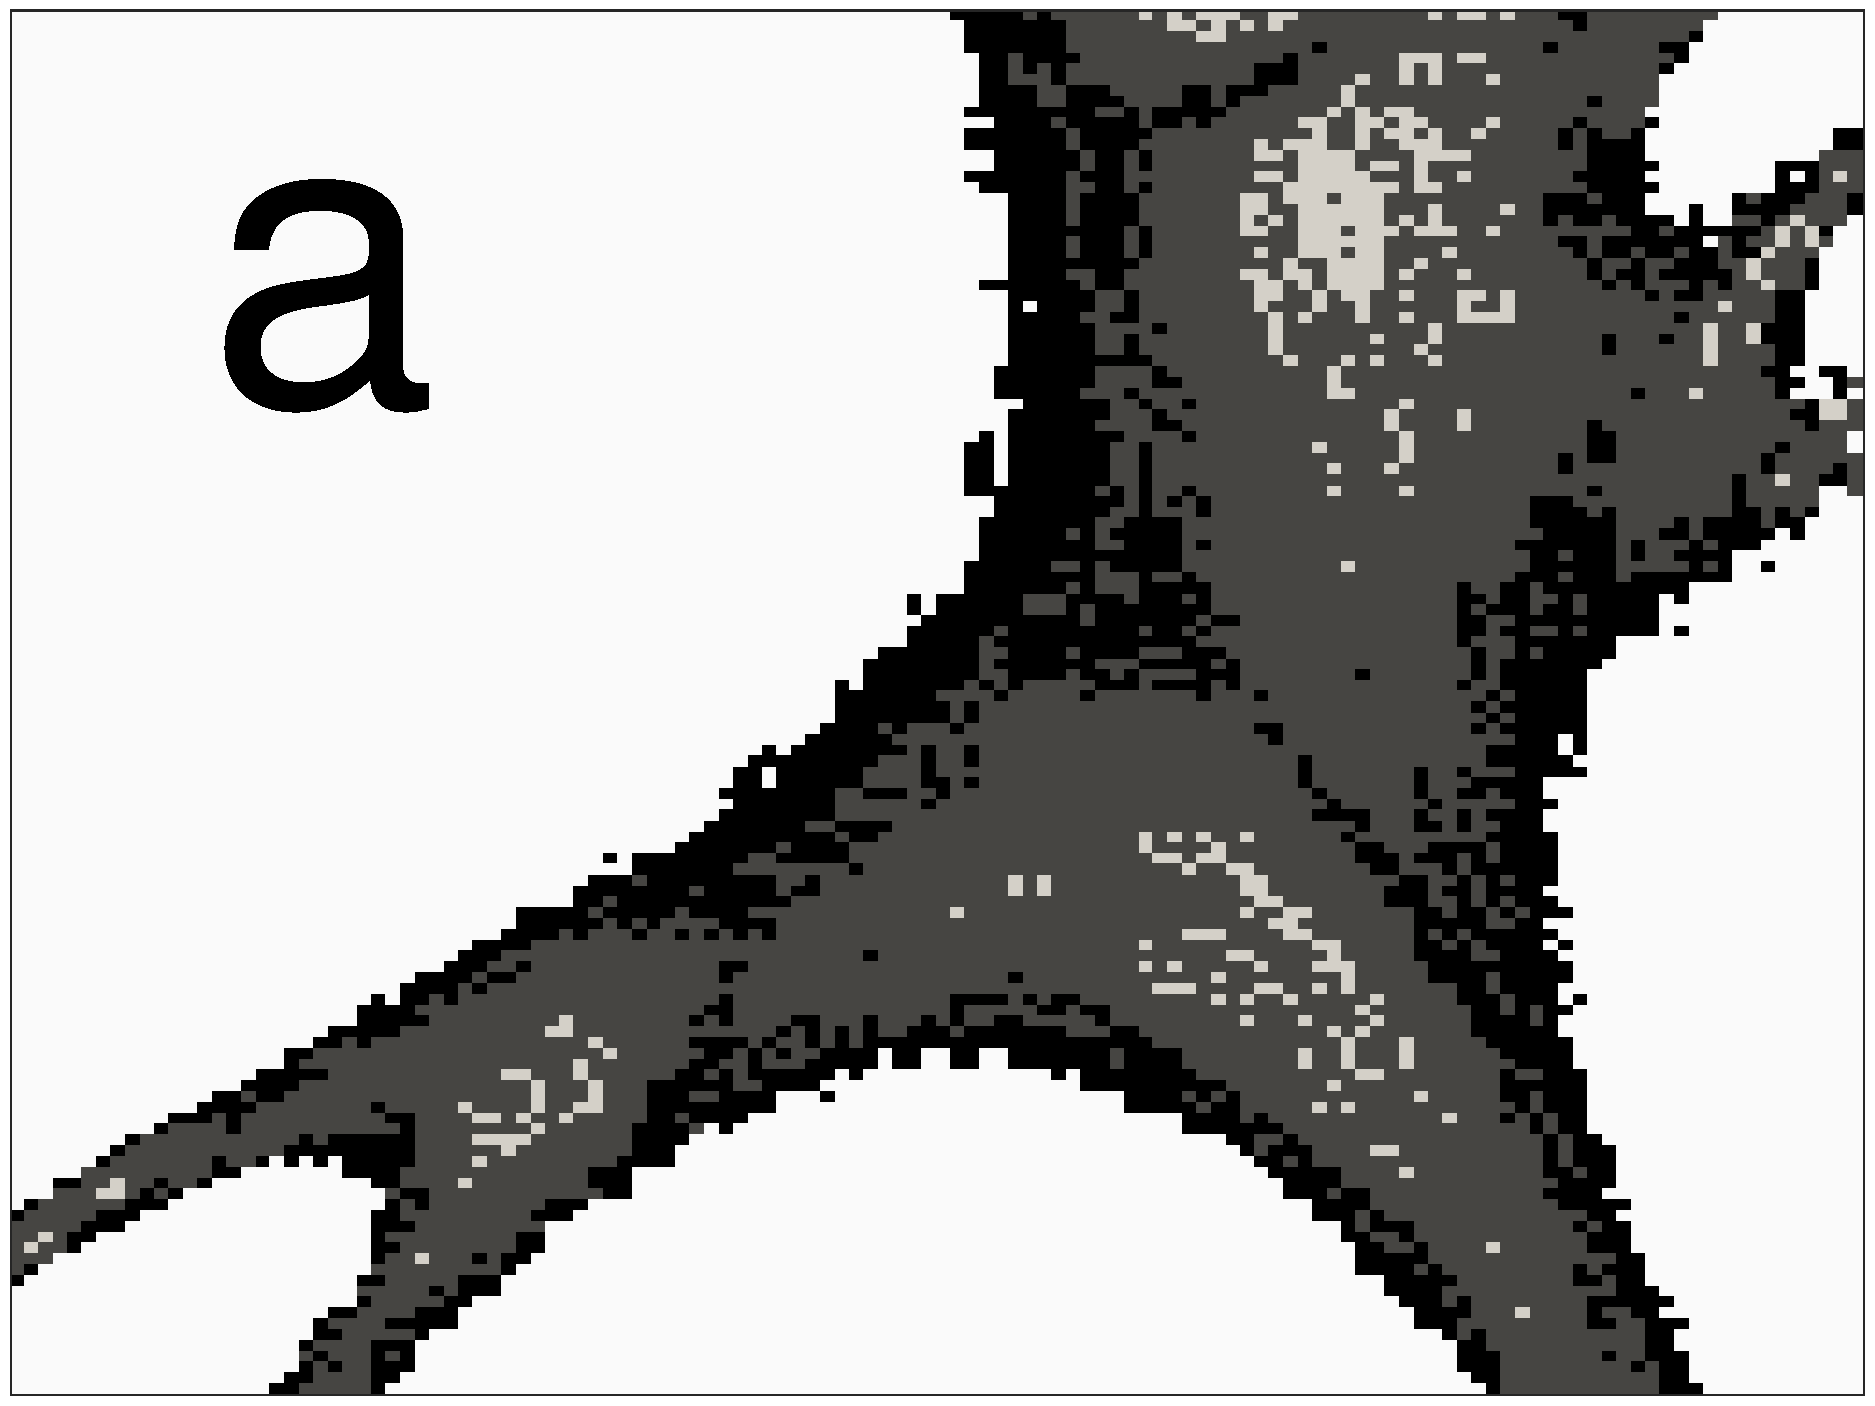
\includegraphics[width=0.3\textwidth]{m5_lu}
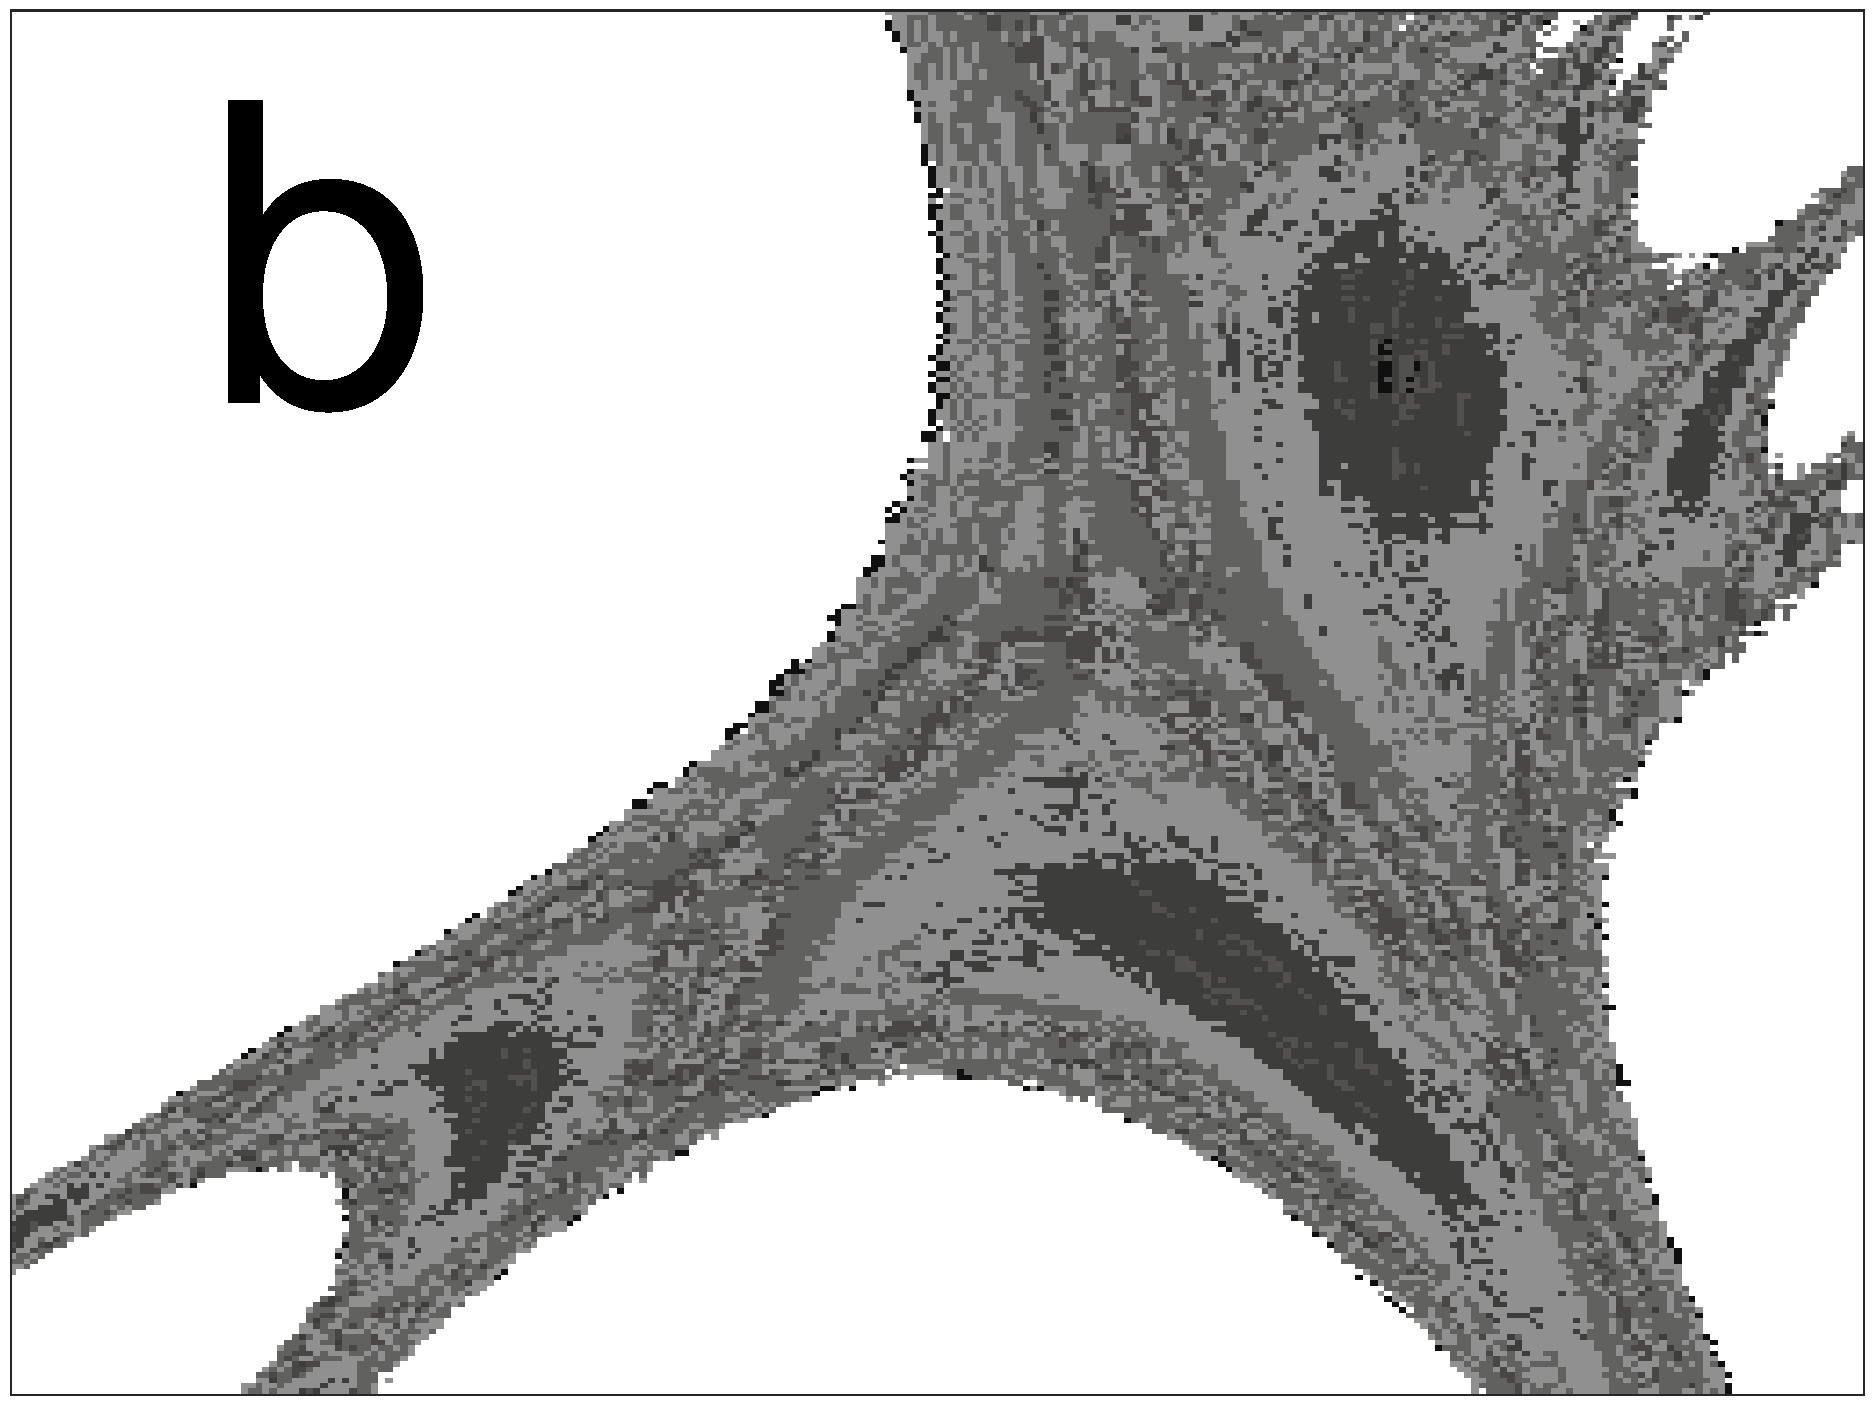
\includegraphics[width=0.3\textwidth]{m6_lu}
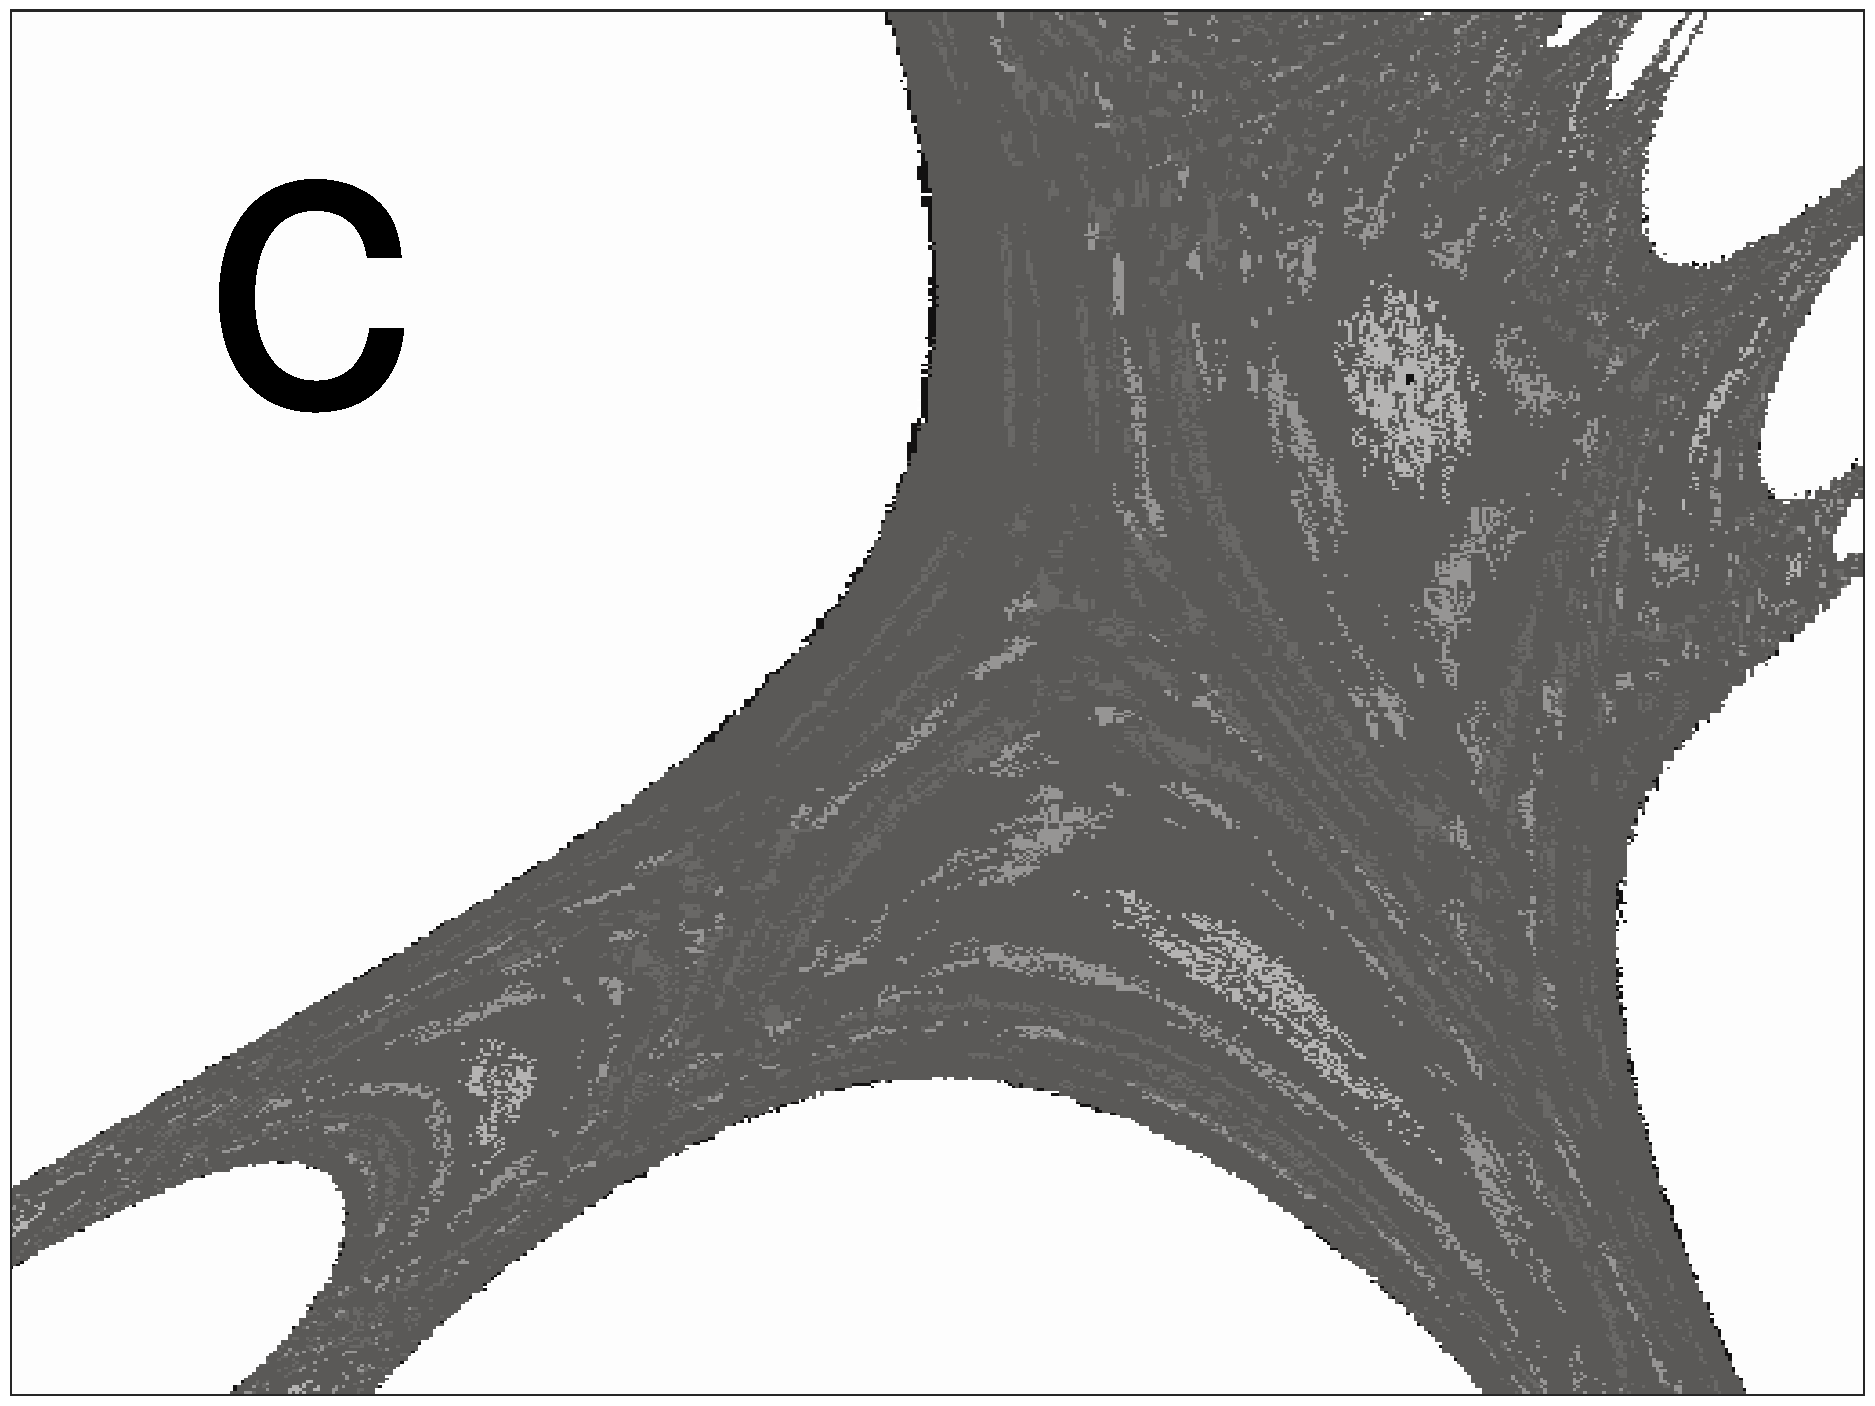
\includegraphics[width=0.3\textwidth]{m7_lu}\\
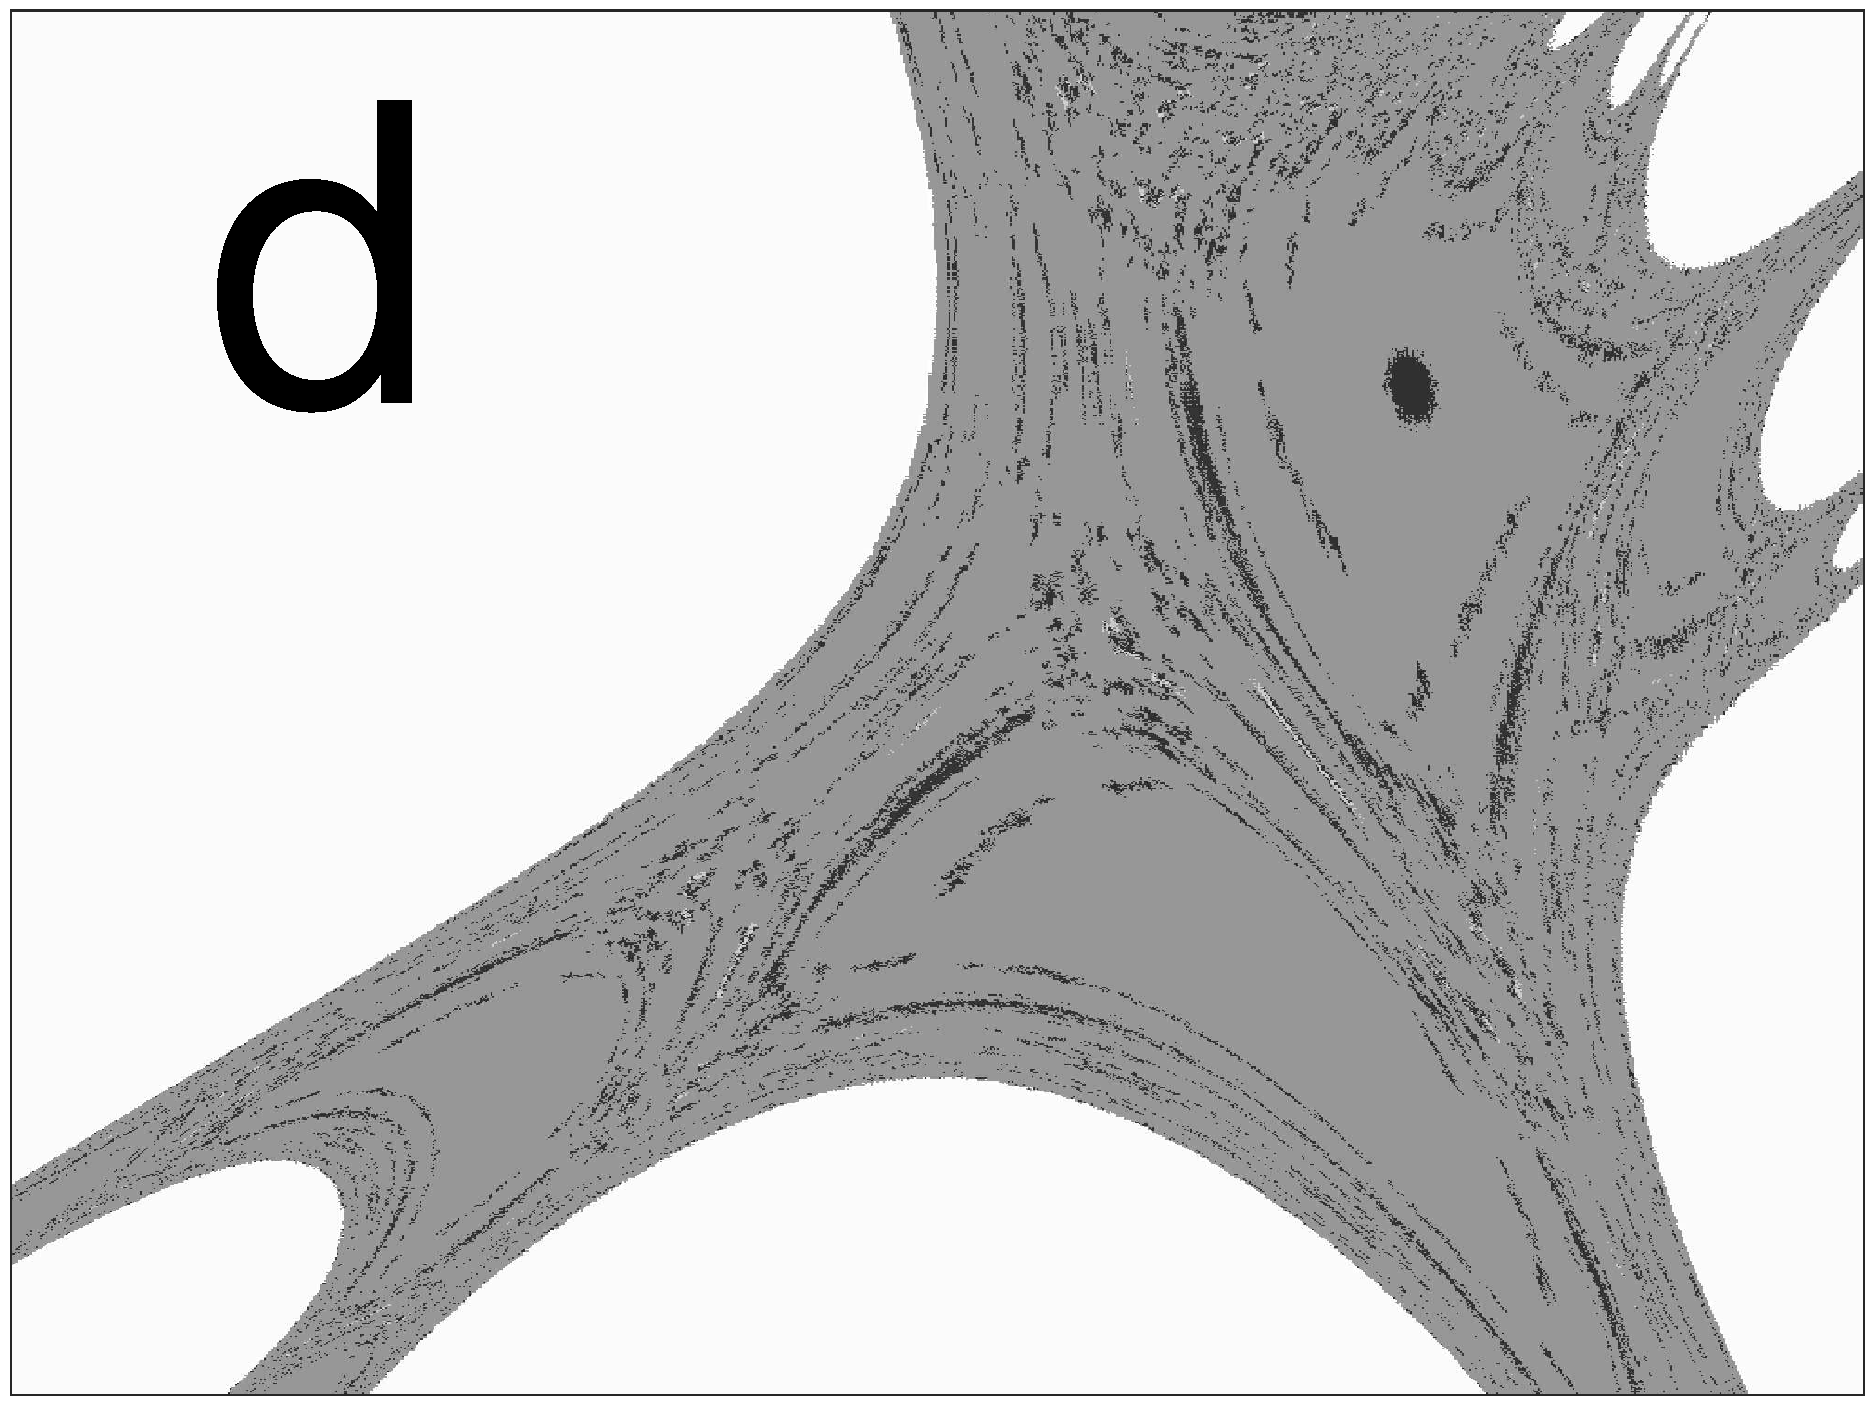
\includegraphics[width=0.3\textwidth]{m8_lu}
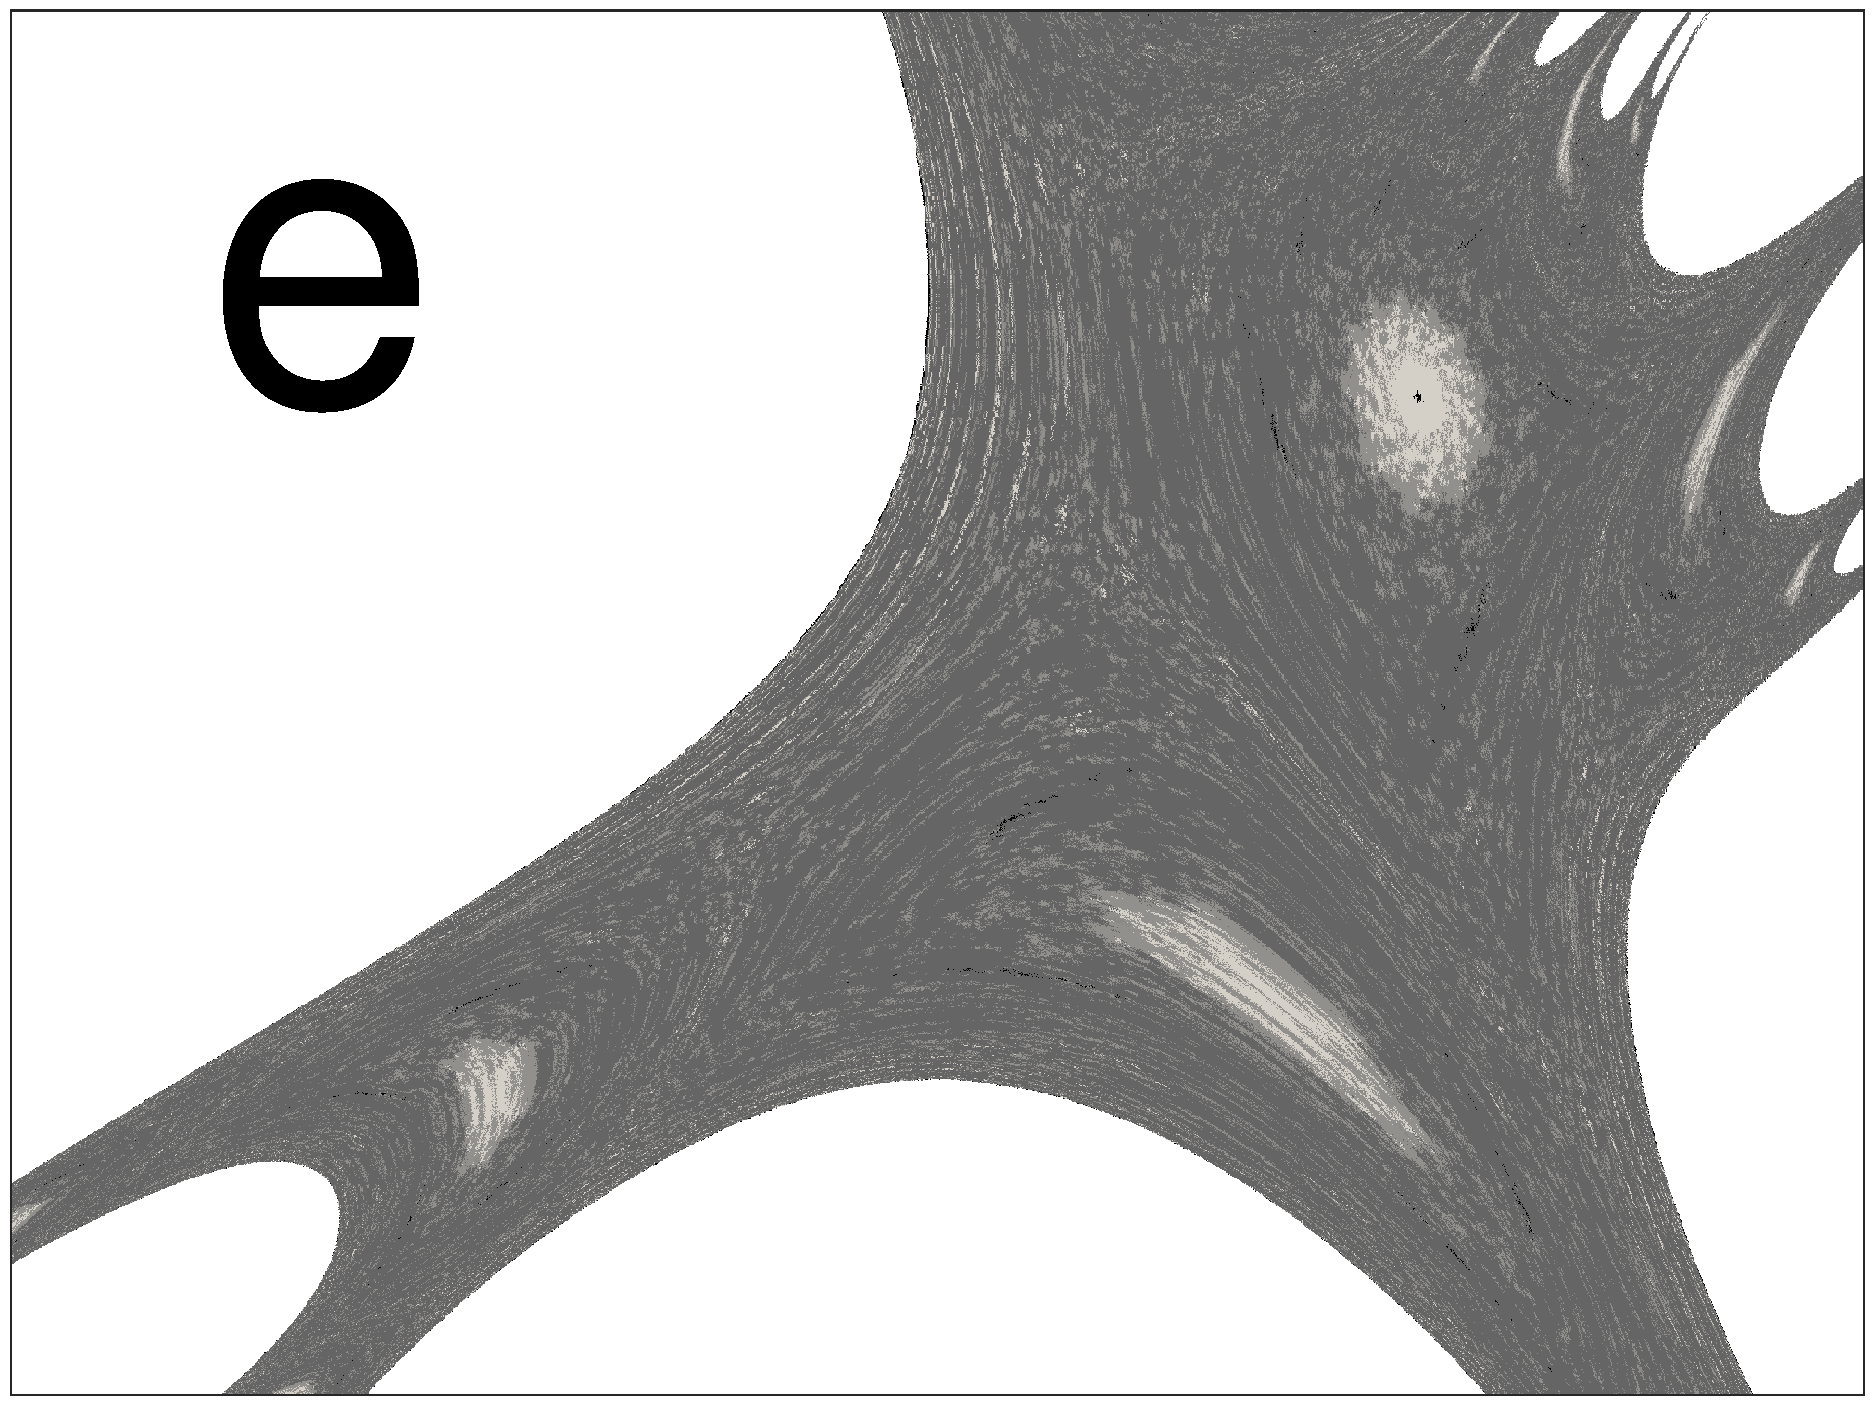
\includegraphics[width=0.3\textwidth]{m9_lu}
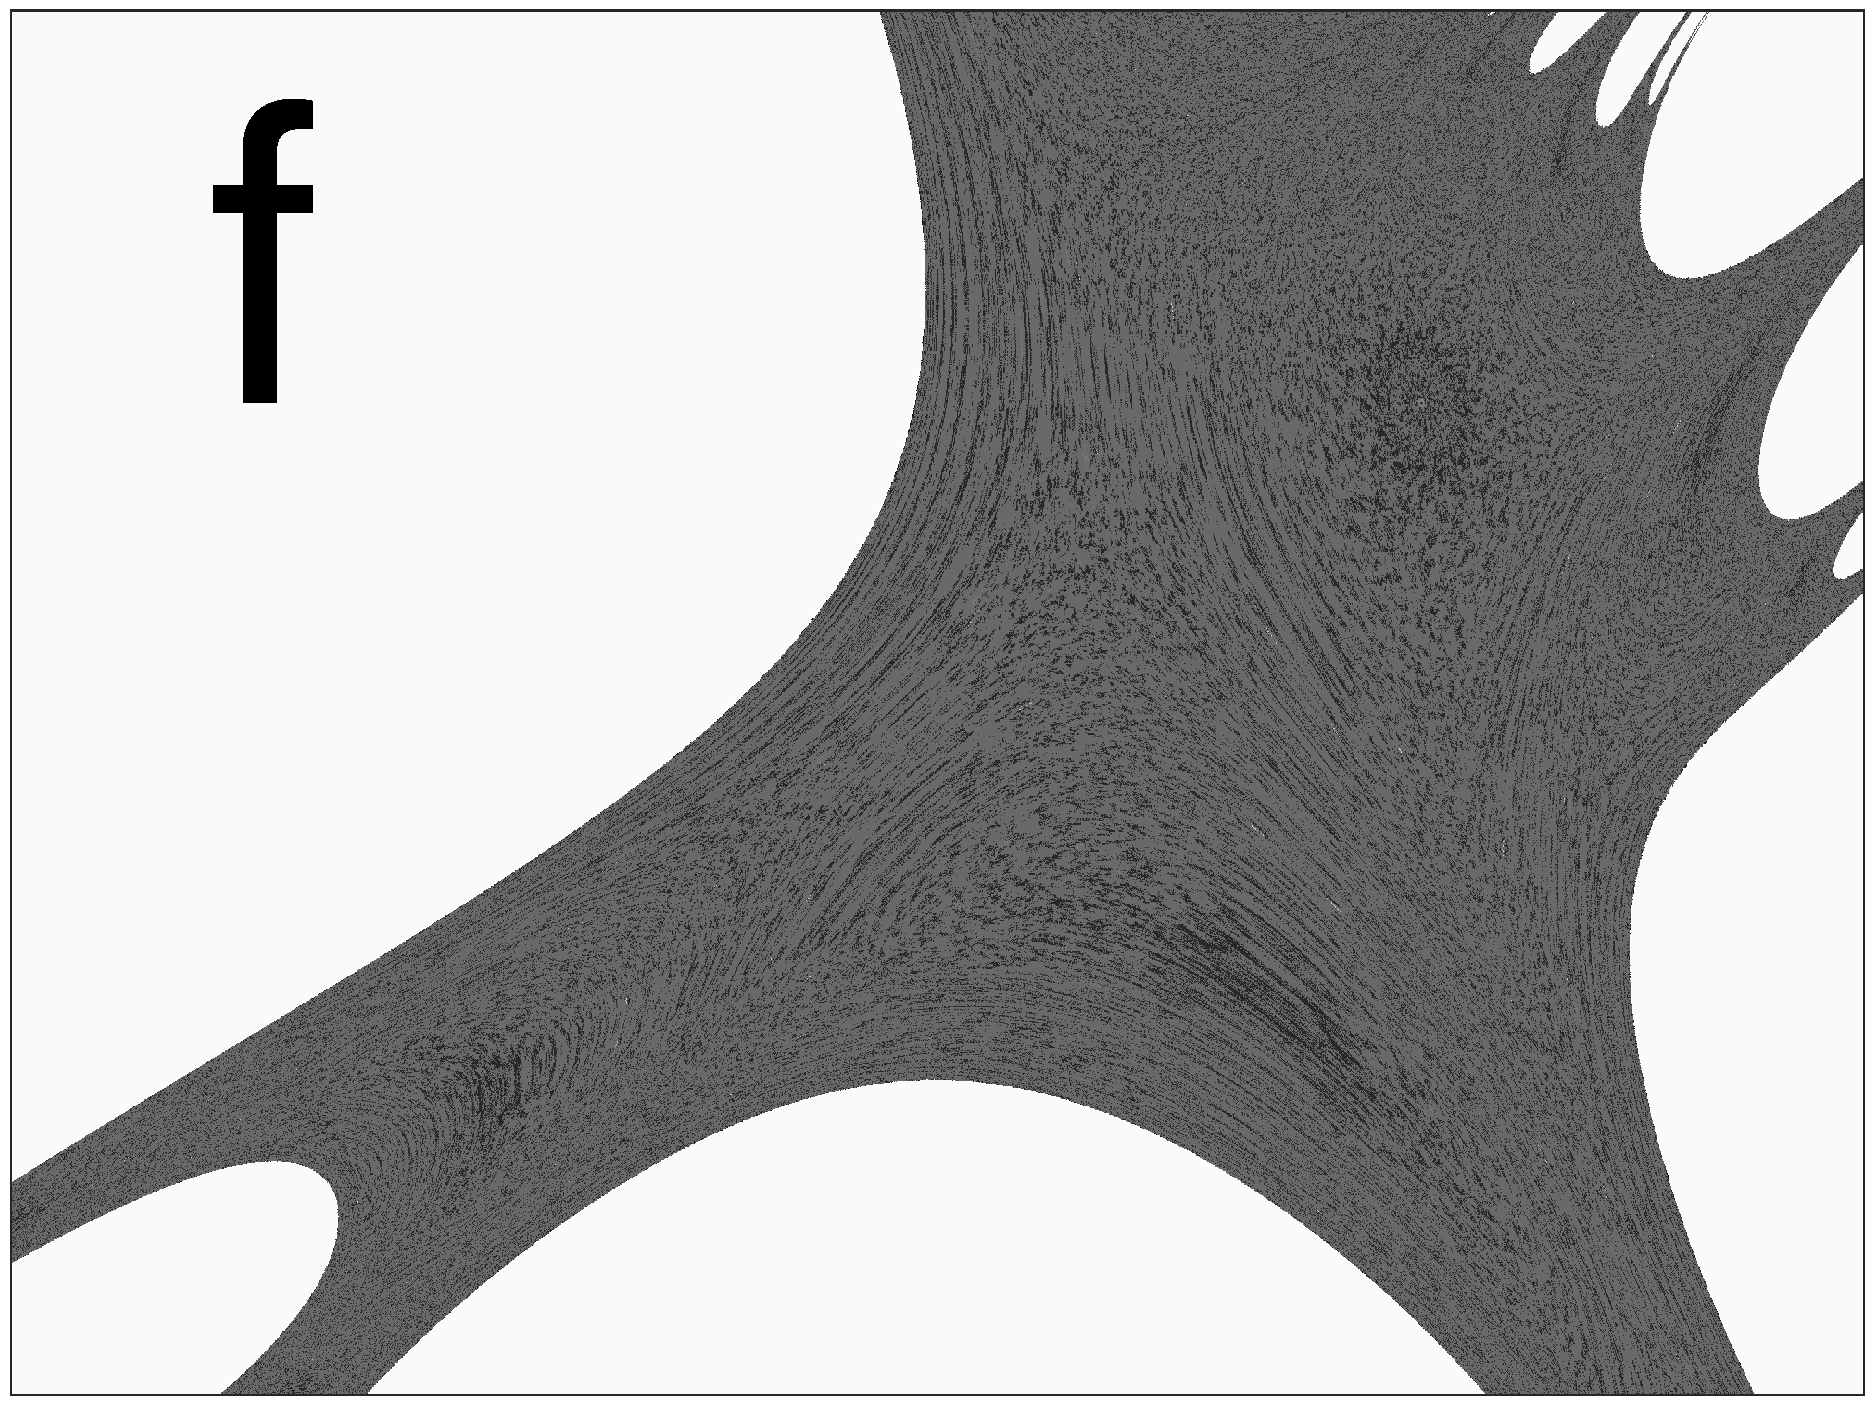
\includegraphics[width=0.3\textwidth]{m10_lu}\\
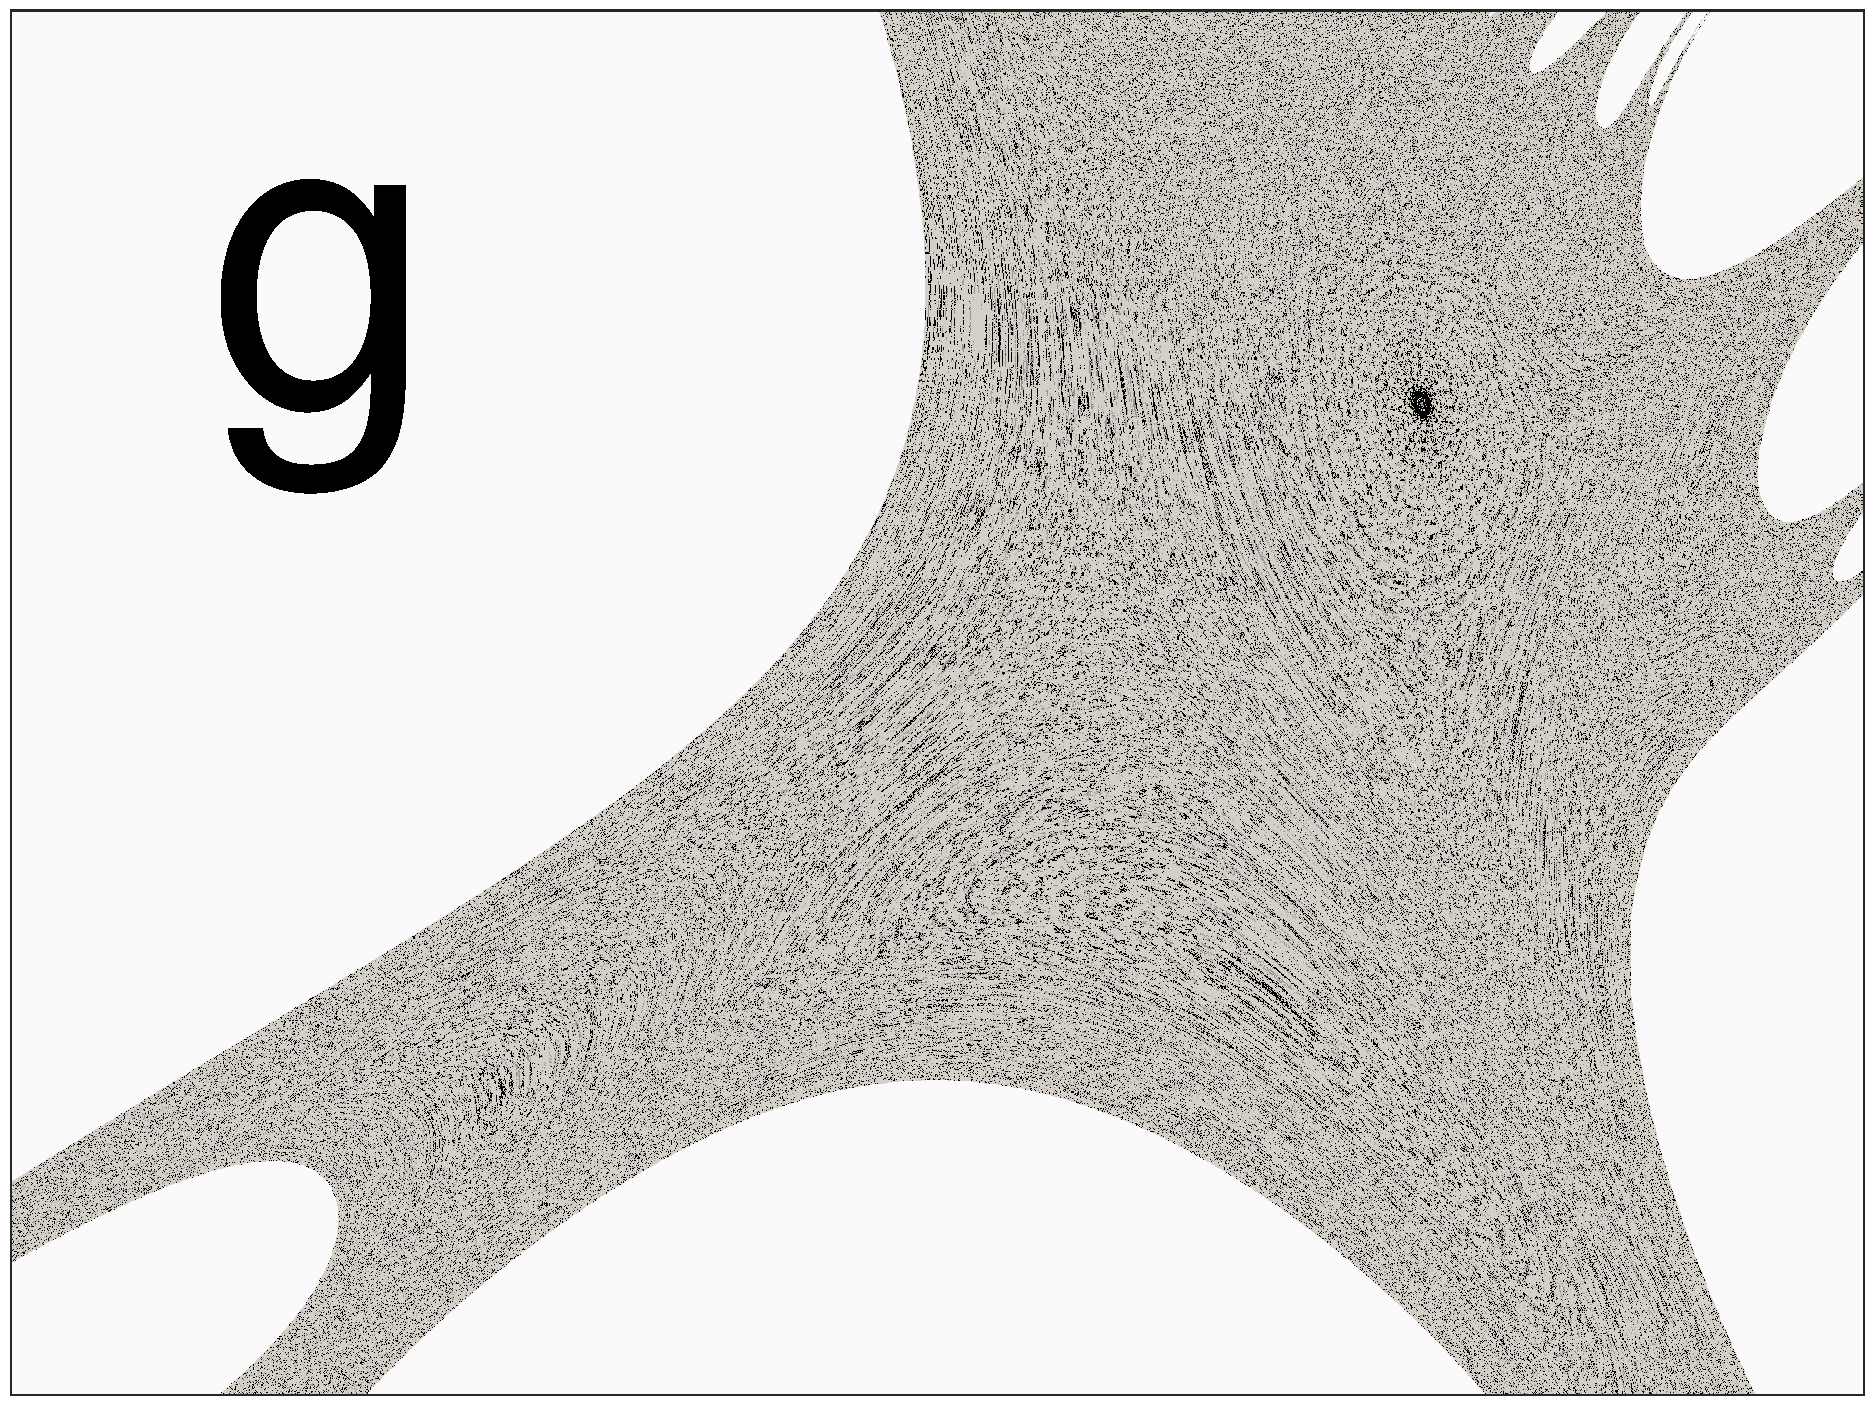
\includegraphics[width=0.3\textwidth]{m11_lu}
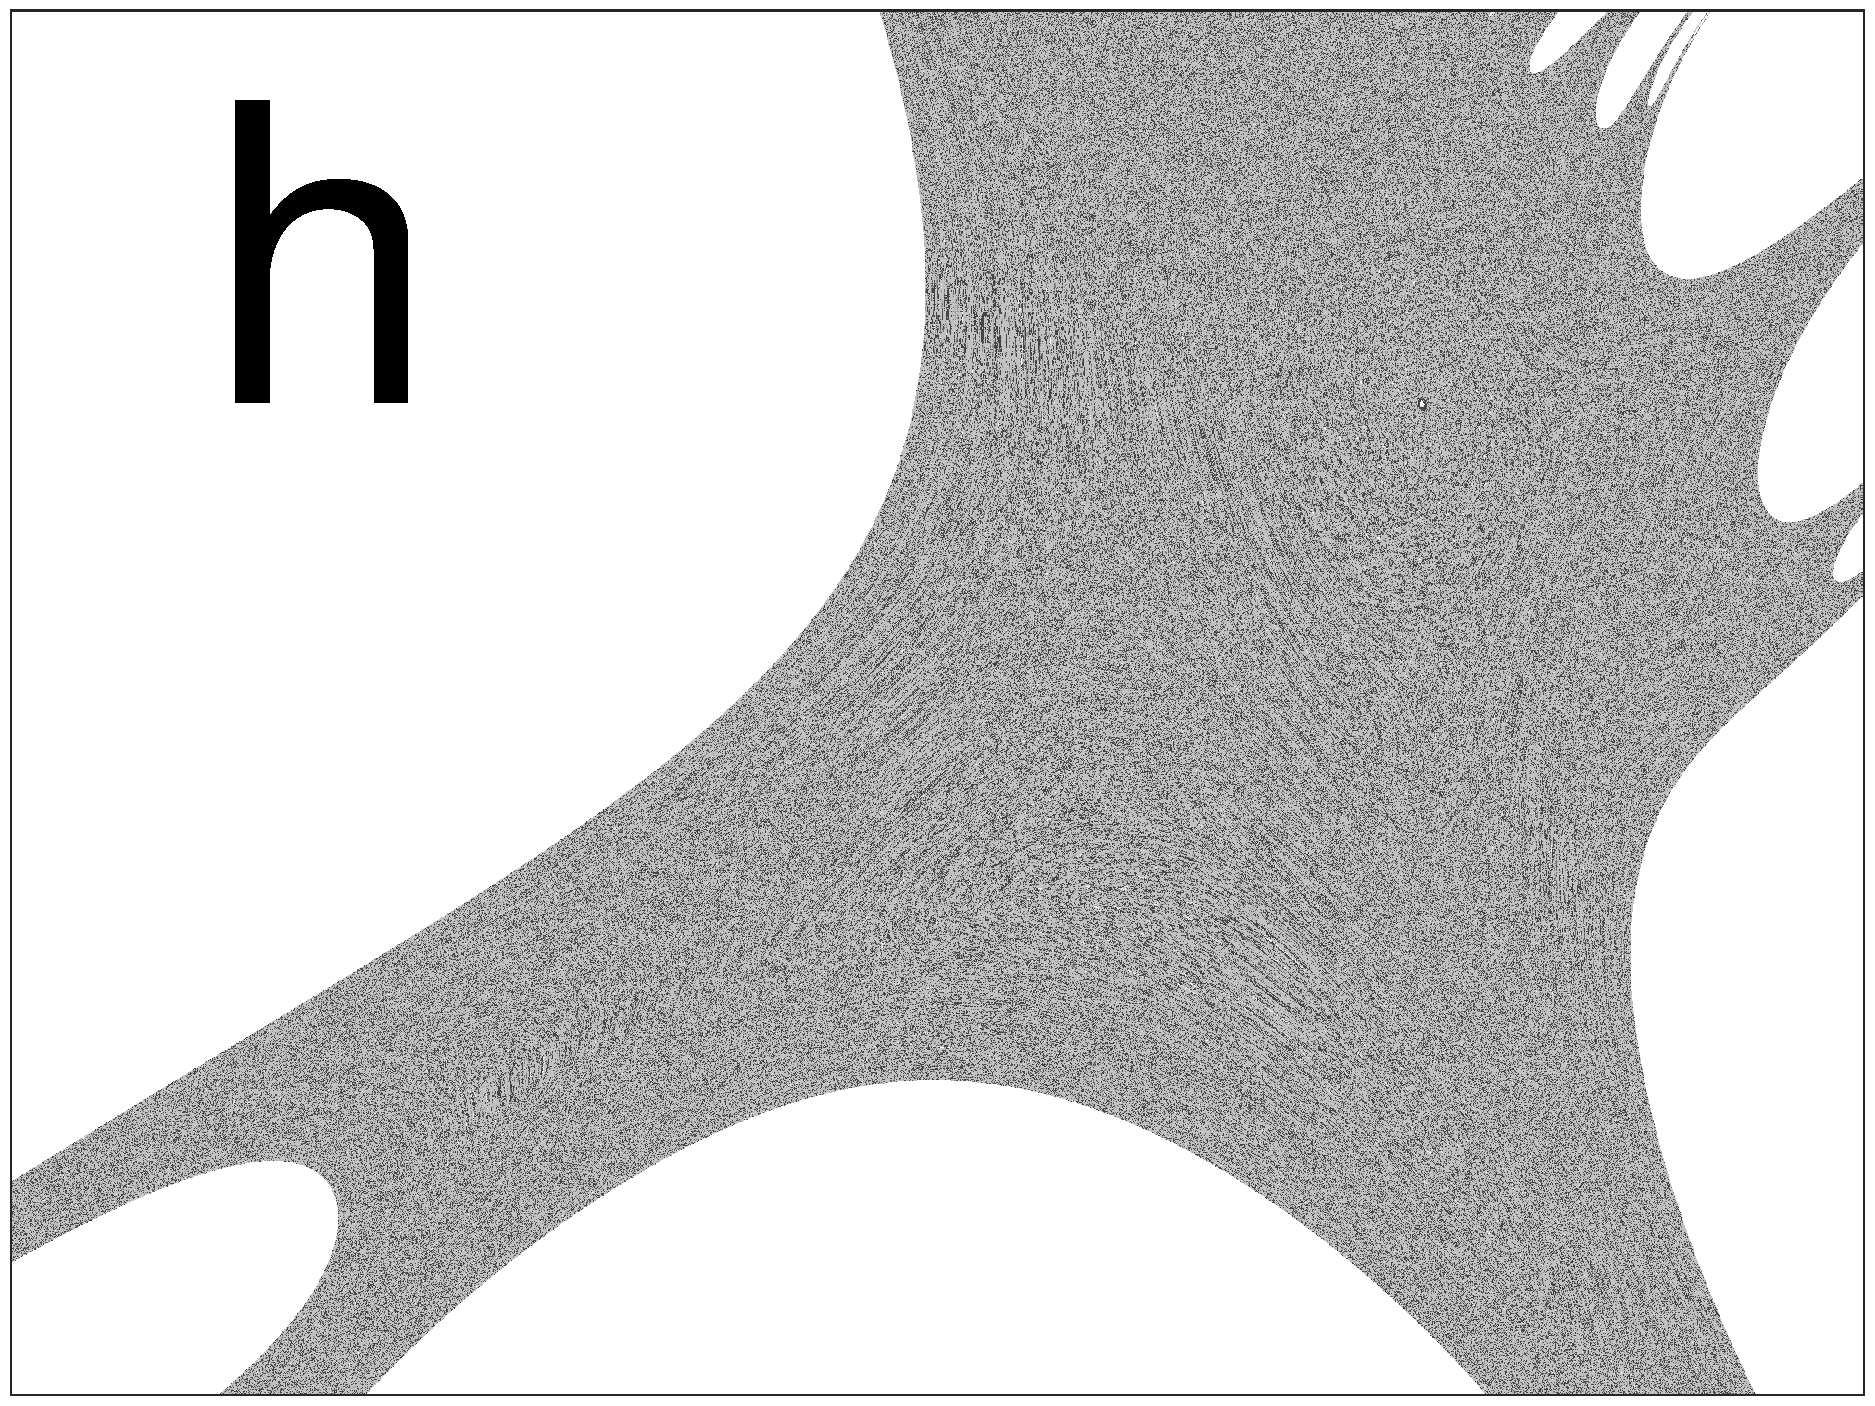
\includegraphics[width=0.3\textwidth]{m12_lu}
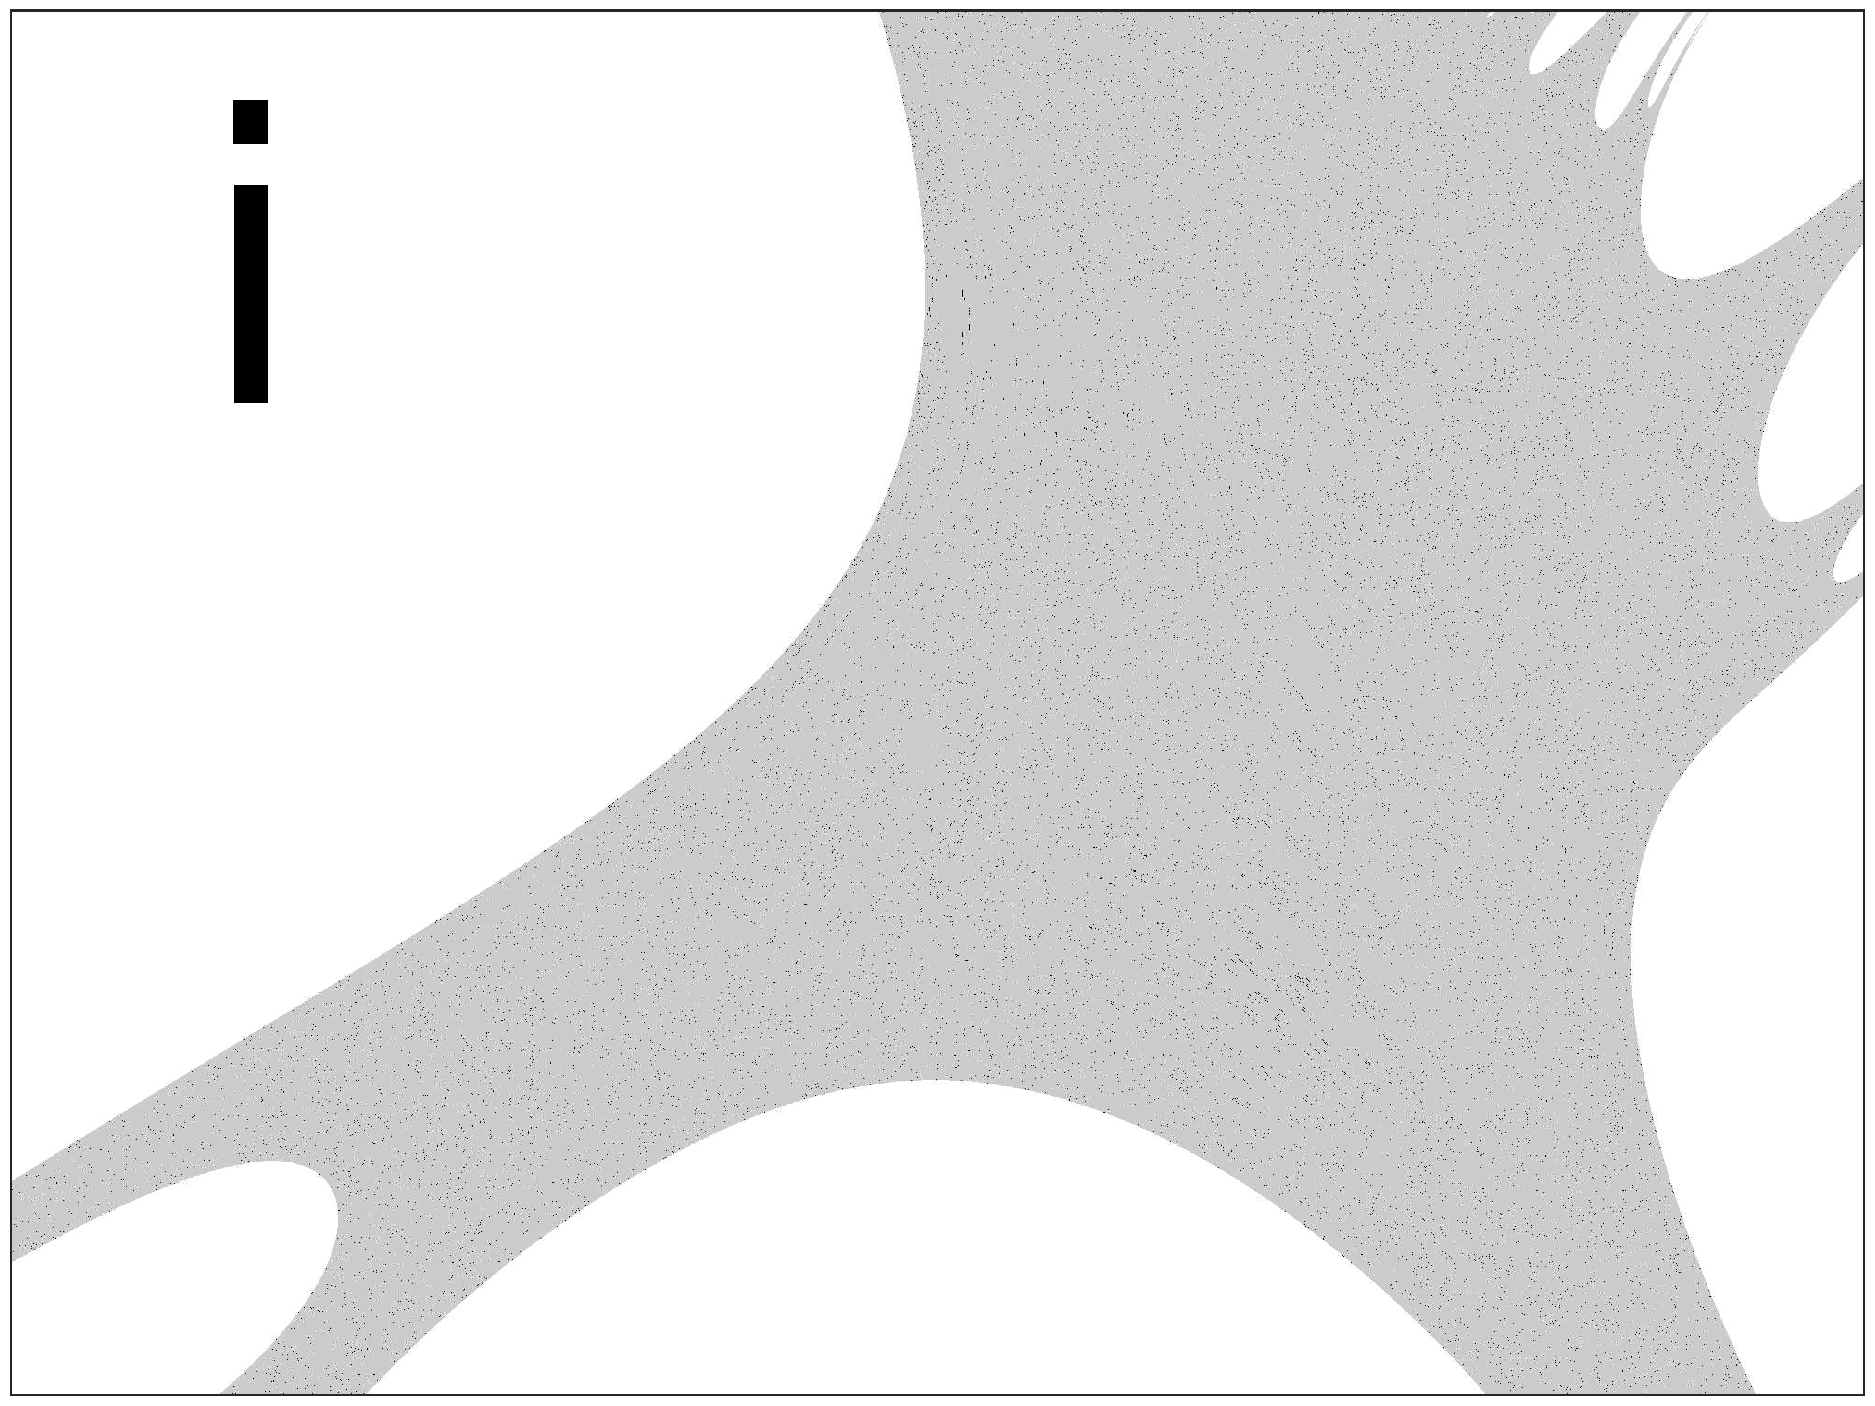
\includegraphics[width=0.3\textwidth]{m13_lu}\\
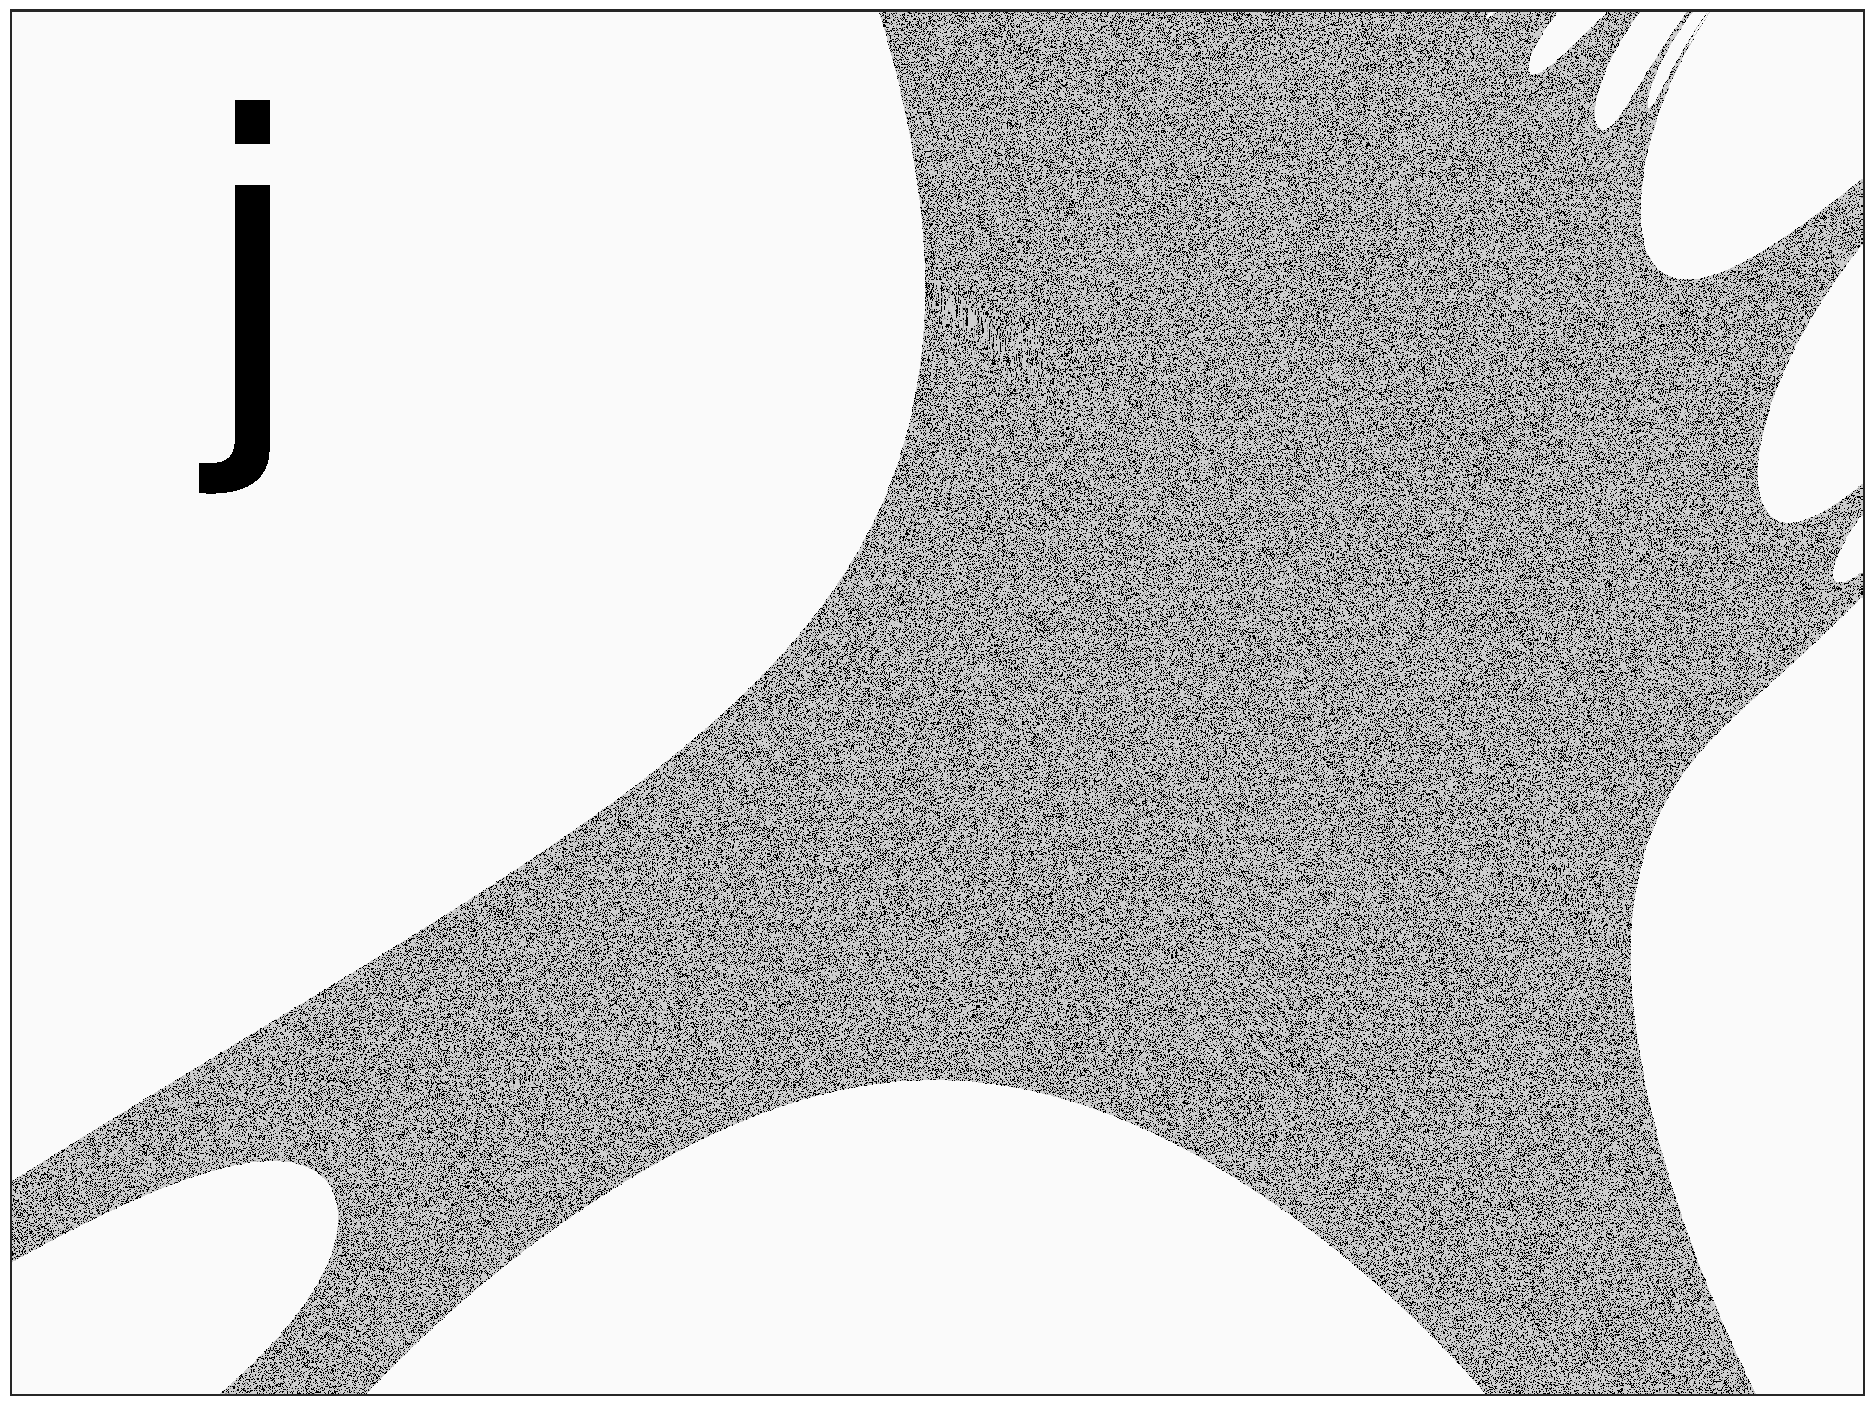
\includegraphics[width=0.3\textwidth]{m14_lu}
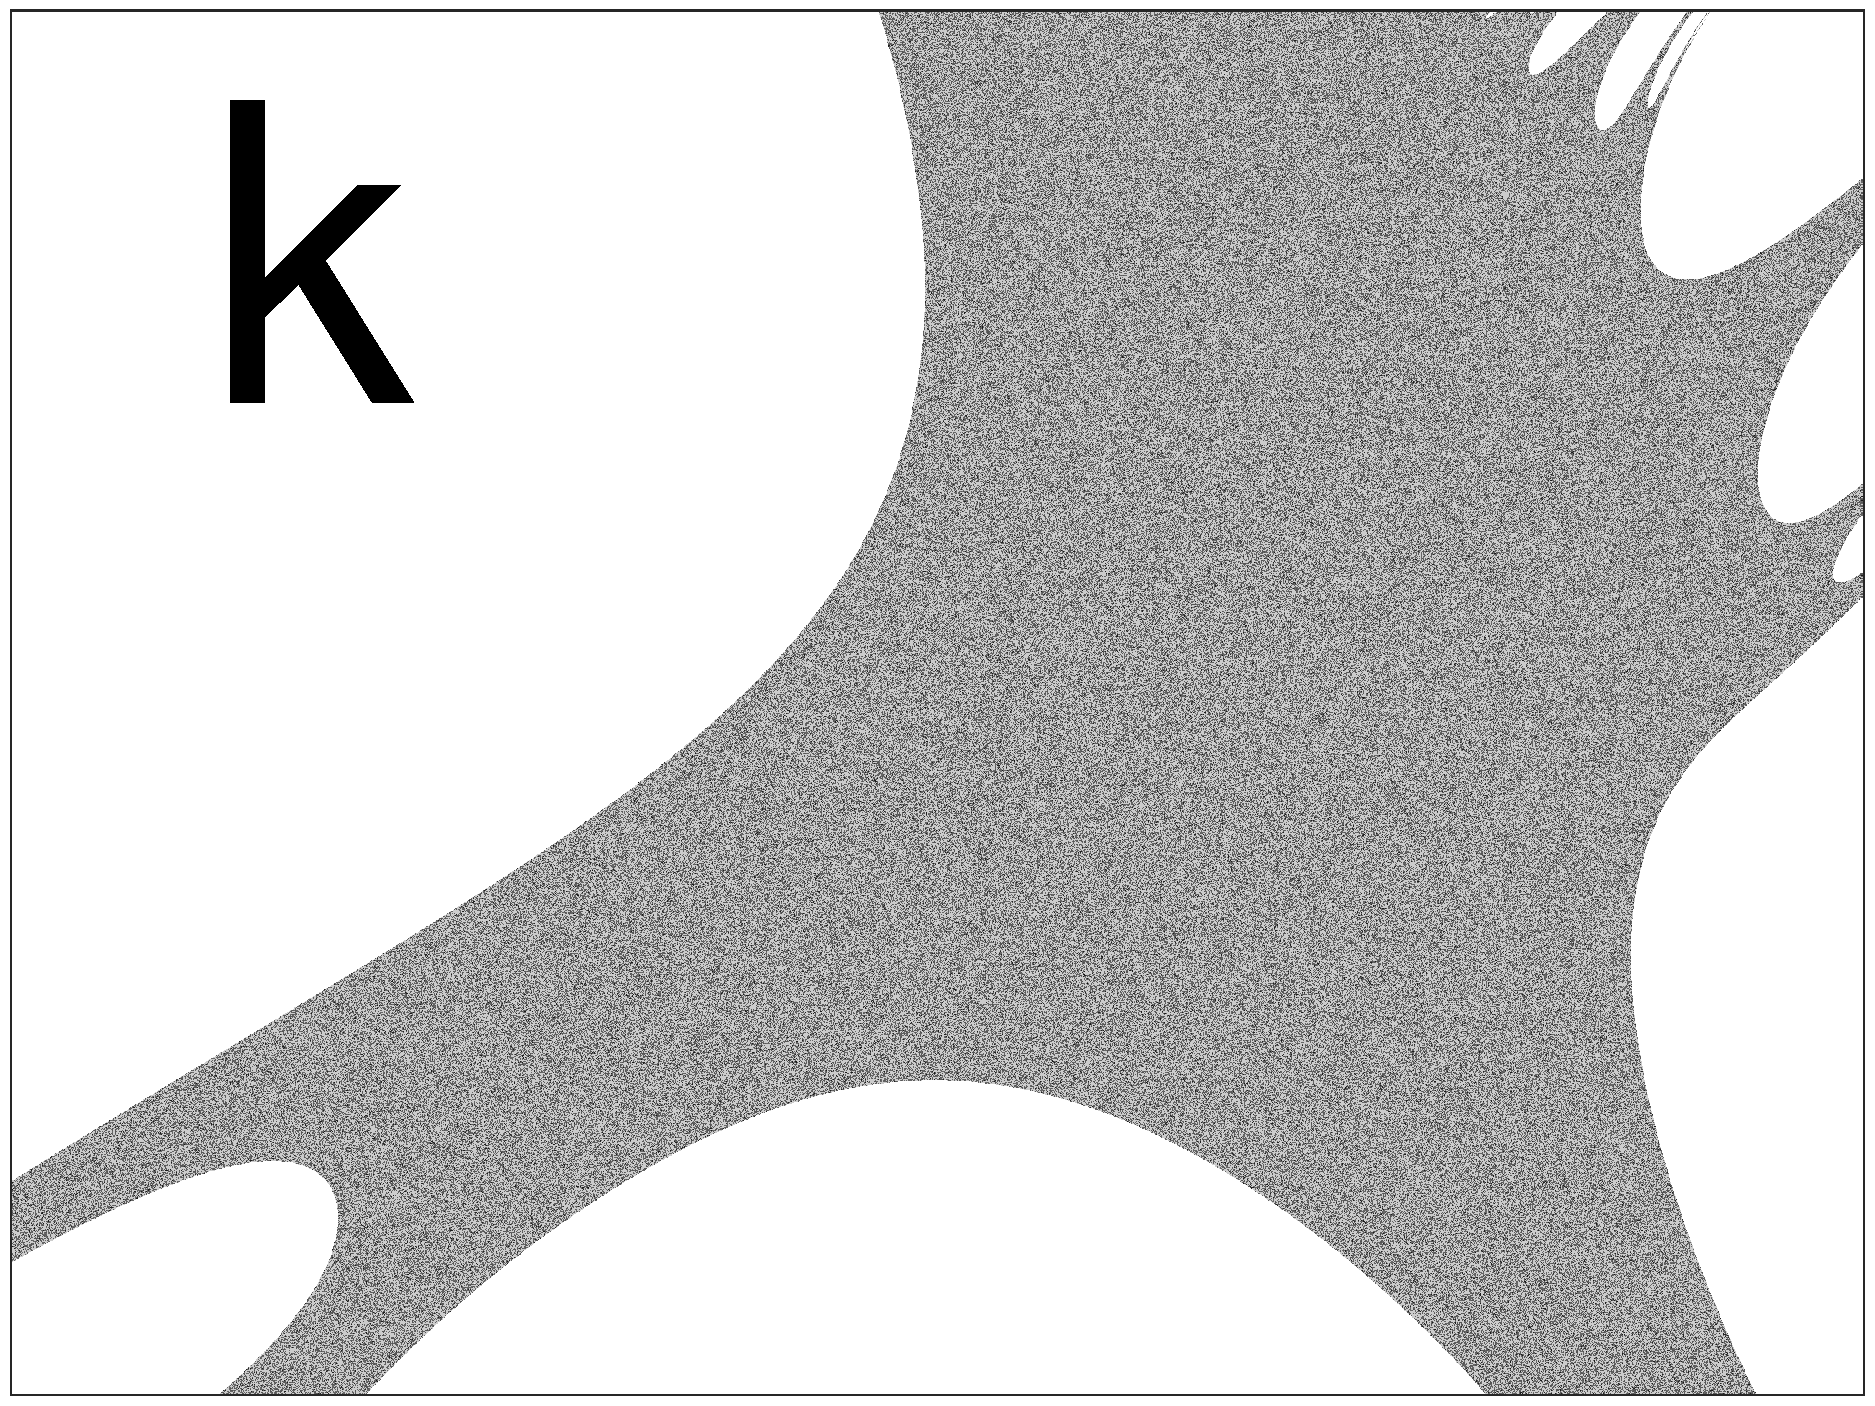
\includegraphics[width=0.3\textwidth]{m17_lu}
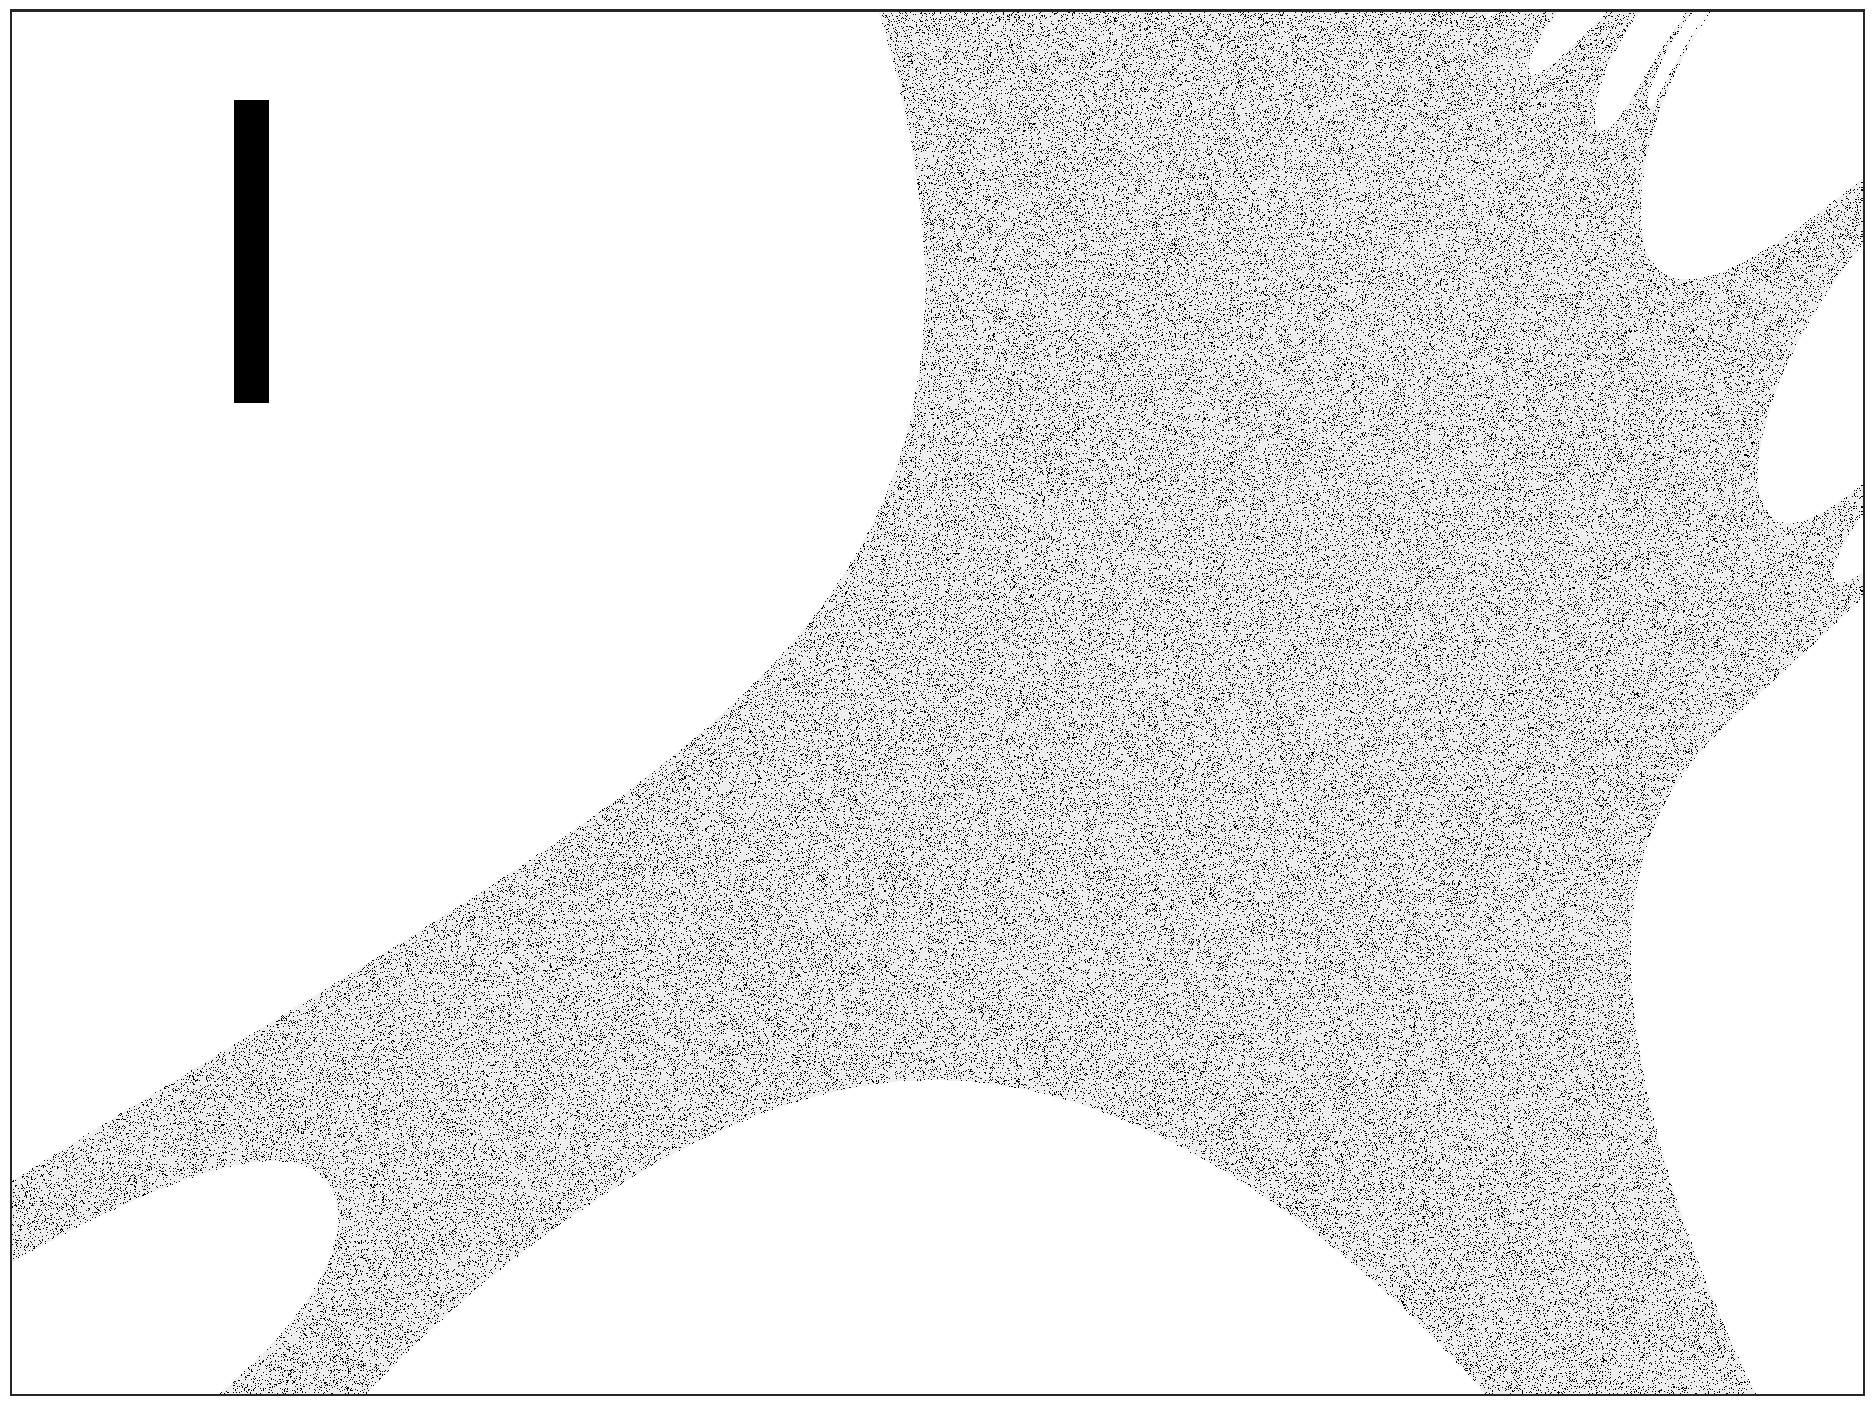
\includegraphics[width=0.3\textwidth]{m18_lu}\\
%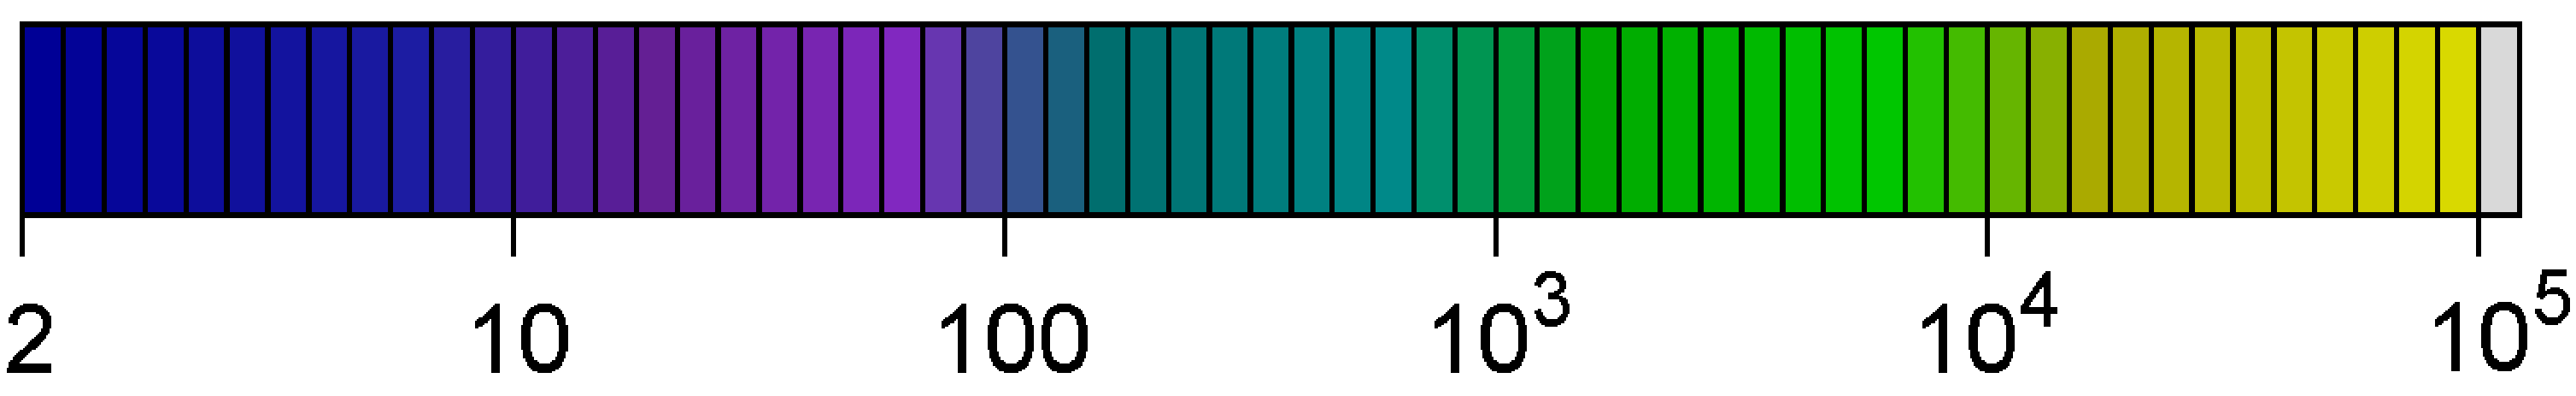
\includegraphics[width=1\textwidth]{ColorMapConEje}
\end{tabular}
\caption{Coexisting areas in attraction domains for: (a) $n_f=5$, (b) $n_f=6$, (c) $n_f=7$, (d) $n_f=8$, (e) $n_f=9$, (f) $n_f=10$, (g) $n_f=11$, (h) $n_f=12$, (i) $n_f=13$, (j) $n_f=14$, (k) $n_f=17$, (l) $n_f=18$.}
\label{fig:avvelo}
\end{figure}

With the purpose of being able to distinguish the different coexisting areas, a diverse range of gray tones have been used on each figure. It must be taken into account that each figure has its own gray range, this means that, for example, an almost white area when $n_f = 5$ (Fig. \ref{fig:avvelo}.a) corresponds to a period of $6$, while a darker area in a figure with higher $n_f$ may correspond to a period higher than a thousand (Fig. \ref{fig:avvelo}.e). These figures allow reflecting the  complex domains of attraction that appear when digitalizing.

It can be seen in Fig. \ref{fig:avvelo} that the smaller the value of $n_f$ the bigger the area of ICs that tends to diverge and to converge to fixed points. As $n_f$ increases, the area of divergent and fixed points decreases.
These figures along with Table \ref{tabla} allows an easy interpretation of the system's behavior. In Table \ref{tabla} the period's lengths that appear in the attractor domain for every $n_f$ are sorted by the more to the less numerous ICs that converges to that cycle. In parentheses it can be seen the percent of occurrence.
Indeed, figures with lower values of $n_f$ present irregular, or rough surfaces, pointing out that different lengths cycles coexist there. For example, for $n_f=5$ there is a prevalence of  short periods cycles. In that case, there exist just two limit cycles, the lighter grey zone corresponds to the attraction domain of the limit cycles of length six, that is the less numerous cycle, according to Table \ref{tabla}, and, the darker zone corresponds to the attraction domain of length two cycle.

Although for $n_f \geqslant 13$ (Figures \ref{fig:avvelo}.i to \ref{fig:avvelo}.l) the attractor appears to be smooth and uniform, however, if a \emph{zoom in} is done to the figures (Fig. \ref{fig:m_zoom}) it can be seen that there are still  cycles with different periods that coexist in the attractor for $n_f=14$,$17$ and $18$.


%==========================zooms in============================
\begin{figure}
\begin{tabular}{cc}
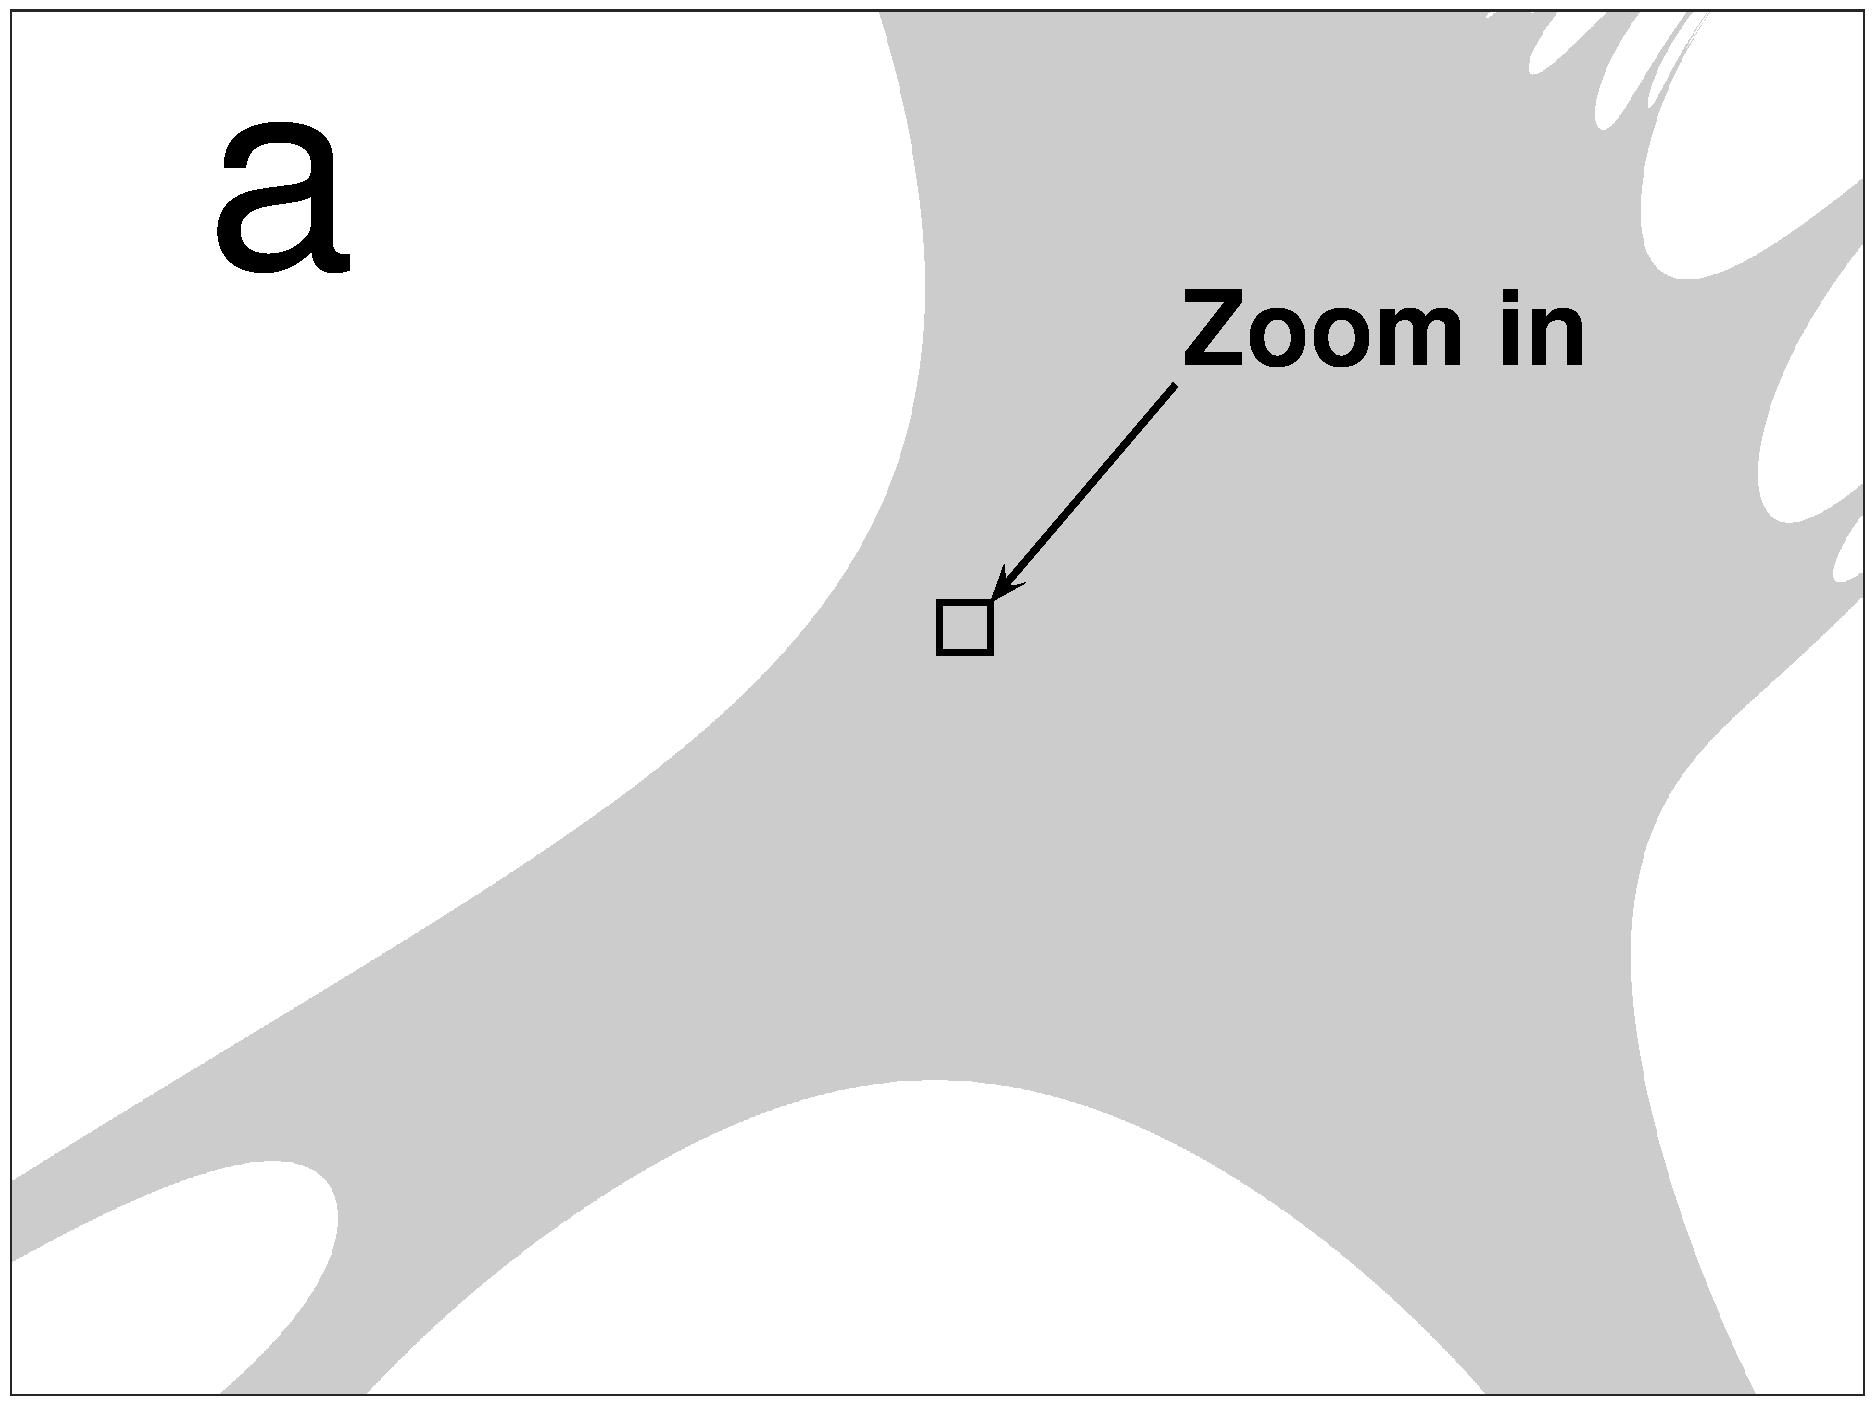
\includegraphics[width=0.48\textwidth]{m_zoom}
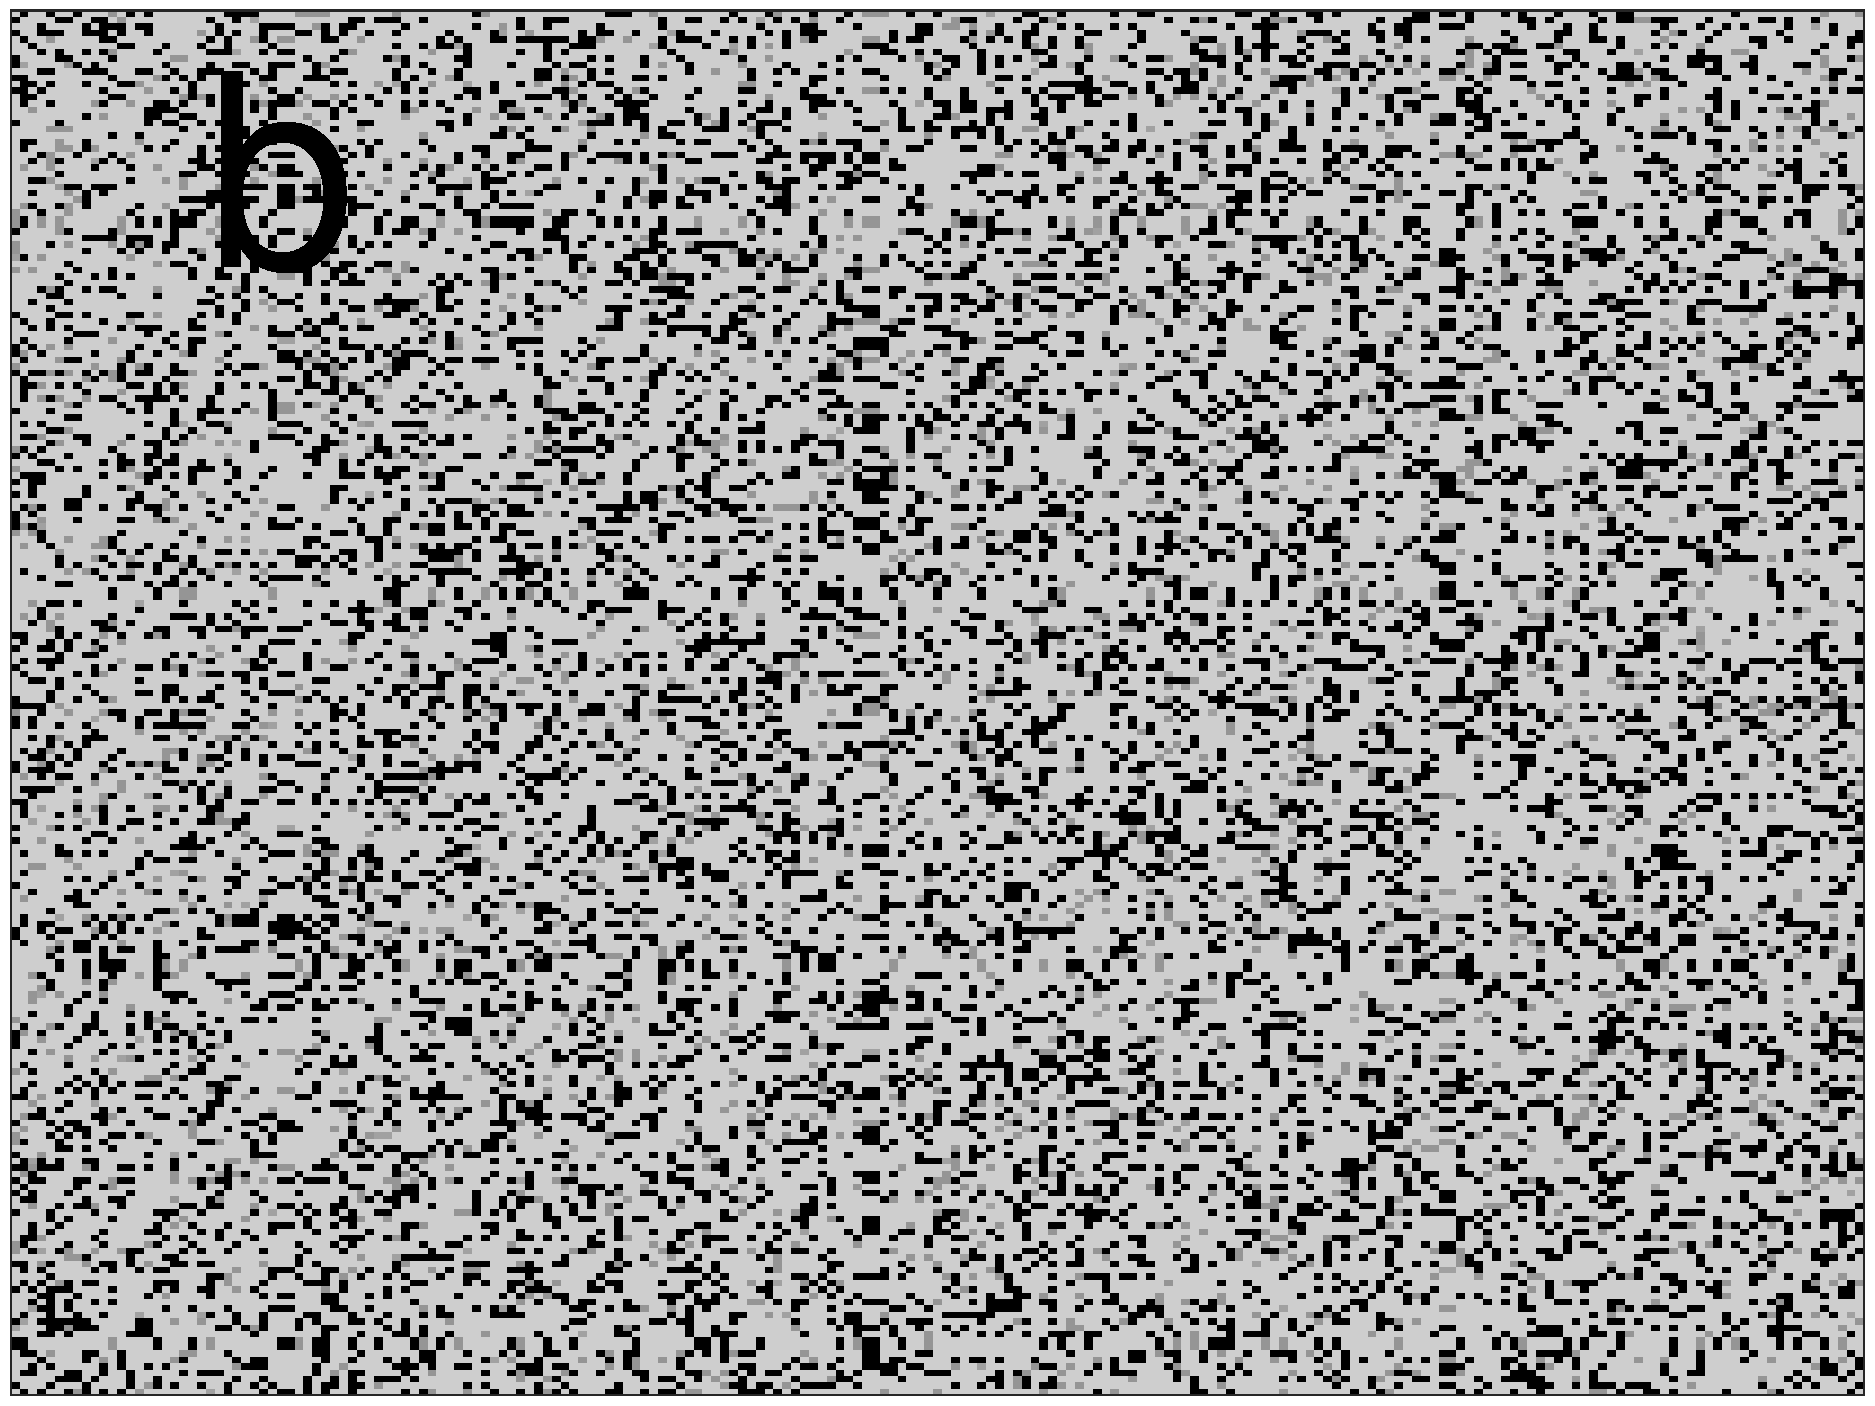
\includegraphics[width=0.48\textwidth]{m14_lu_zoom}\\
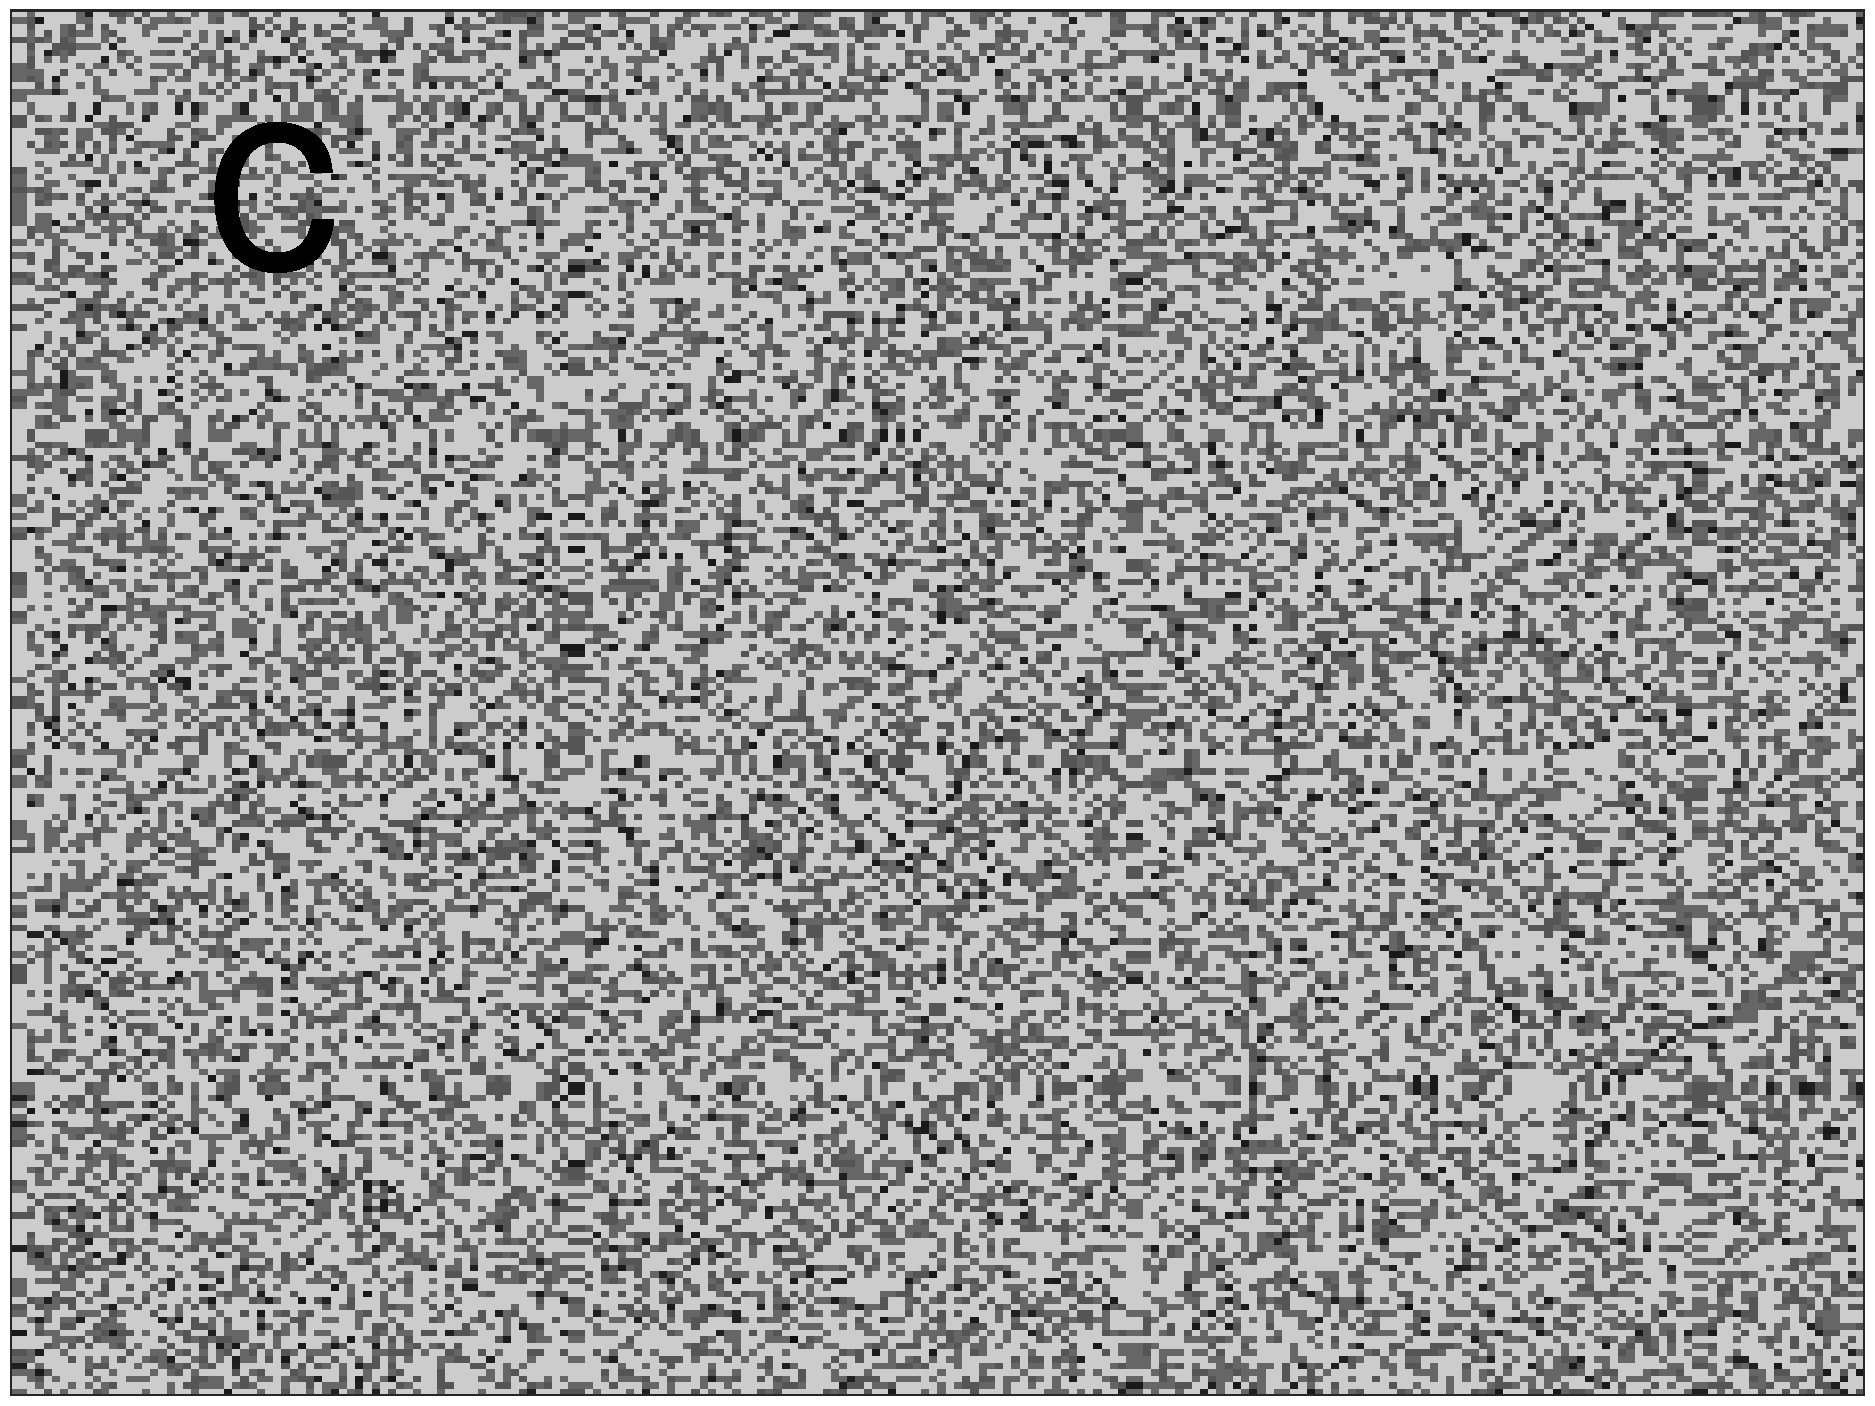
\includegraphics[width=0.48\textwidth]{m17_lu_zoom}
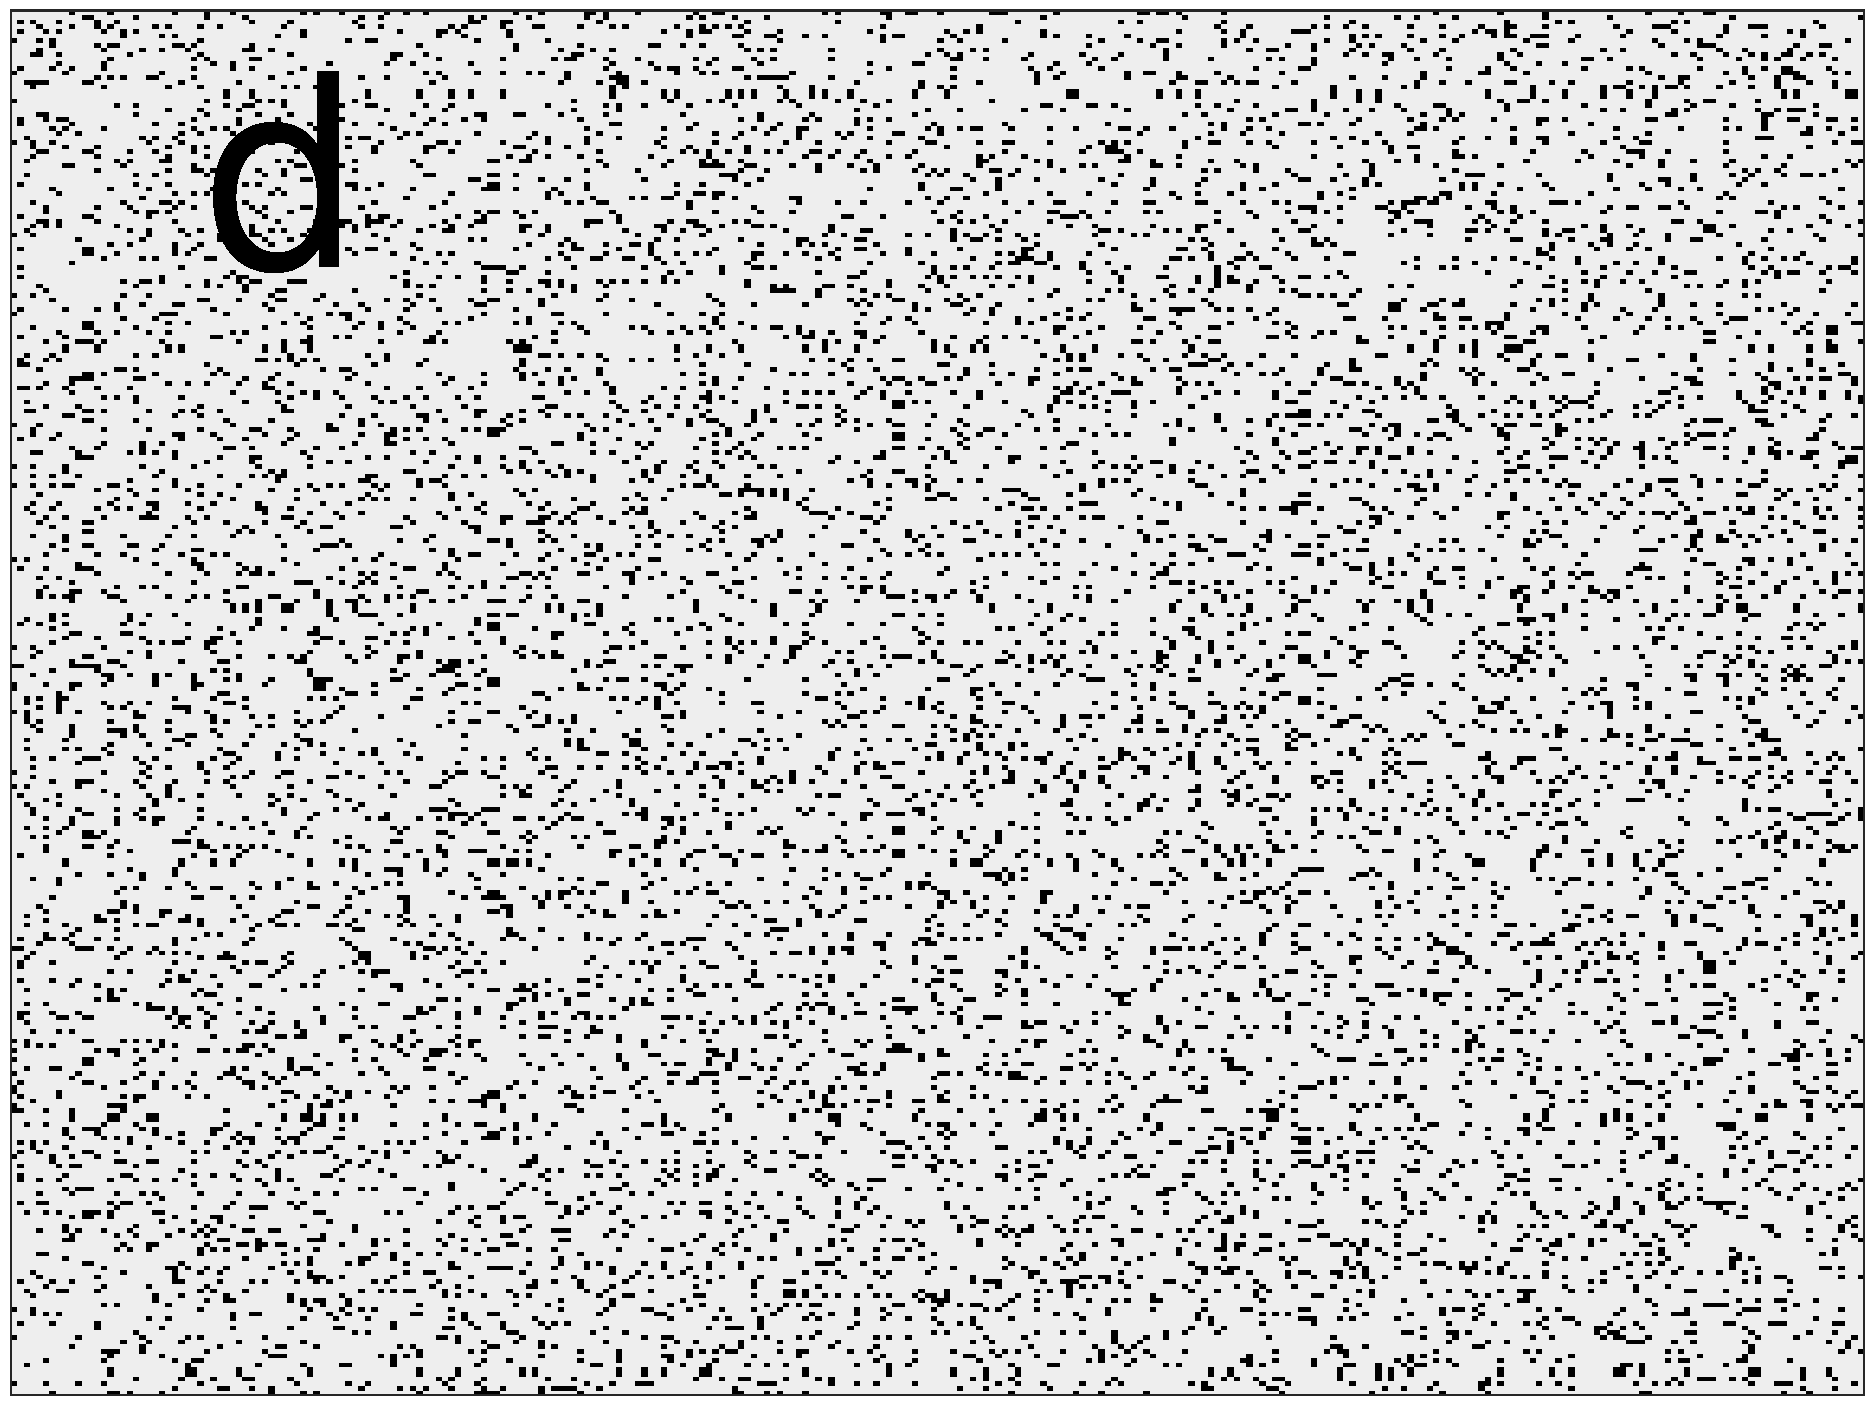
\includegraphics[width=0.48\textwidth]{m18_lu_zoom}
\end{tabular}
\caption{Enlarged views of sections of the attraction domains for higher values of $n_f$:
(a) Rectangular section of the attraction domain to be zoomed in; (b)  $n_f=14$ zoom; (c) $n_f=17$ zoom;  (d) $n_f=18$ zoom.}
\label{fig:m_zoom}
\end{figure}
%============================================================================================

Nevertheless, when we want to make a general comparison of what happens to the periods when the precisions are varied a color scale is required, see Fig. \ref{fig:m}.
% ==DOMINIOS DE ATRACCION DE ATRACTOR 2PARA DISTINTO NUMERO DE BITS  
% SALTEAMOS 15 Y 16 PORQUE DAN MUY PARECIDOS A 14 Y 17
\begin{figure}
\centering
\begin{tabular}{cc}
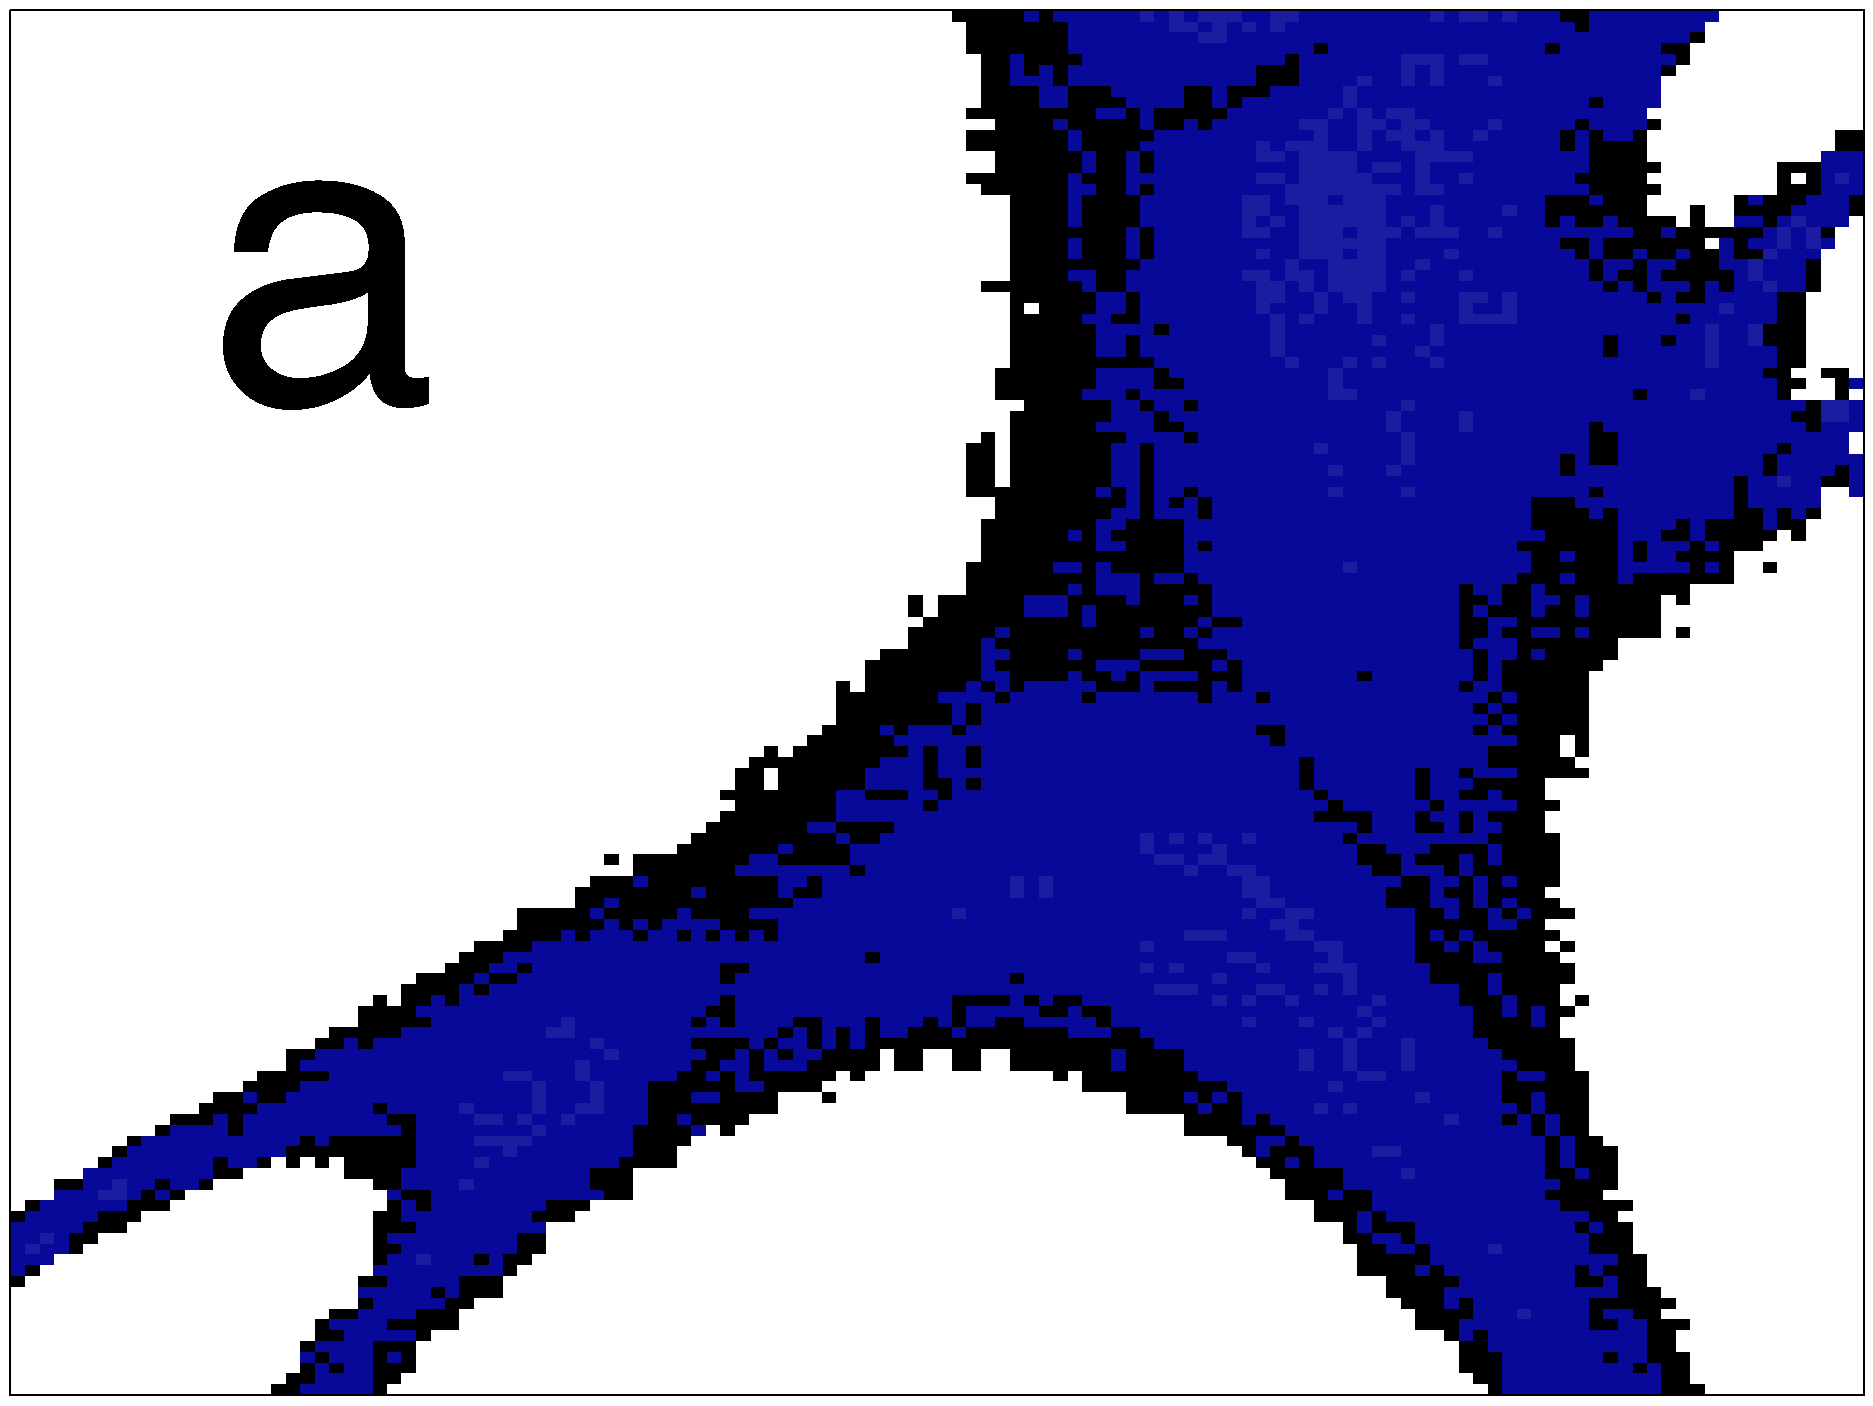
\includegraphics[width=0.3\textwidth]{m5}
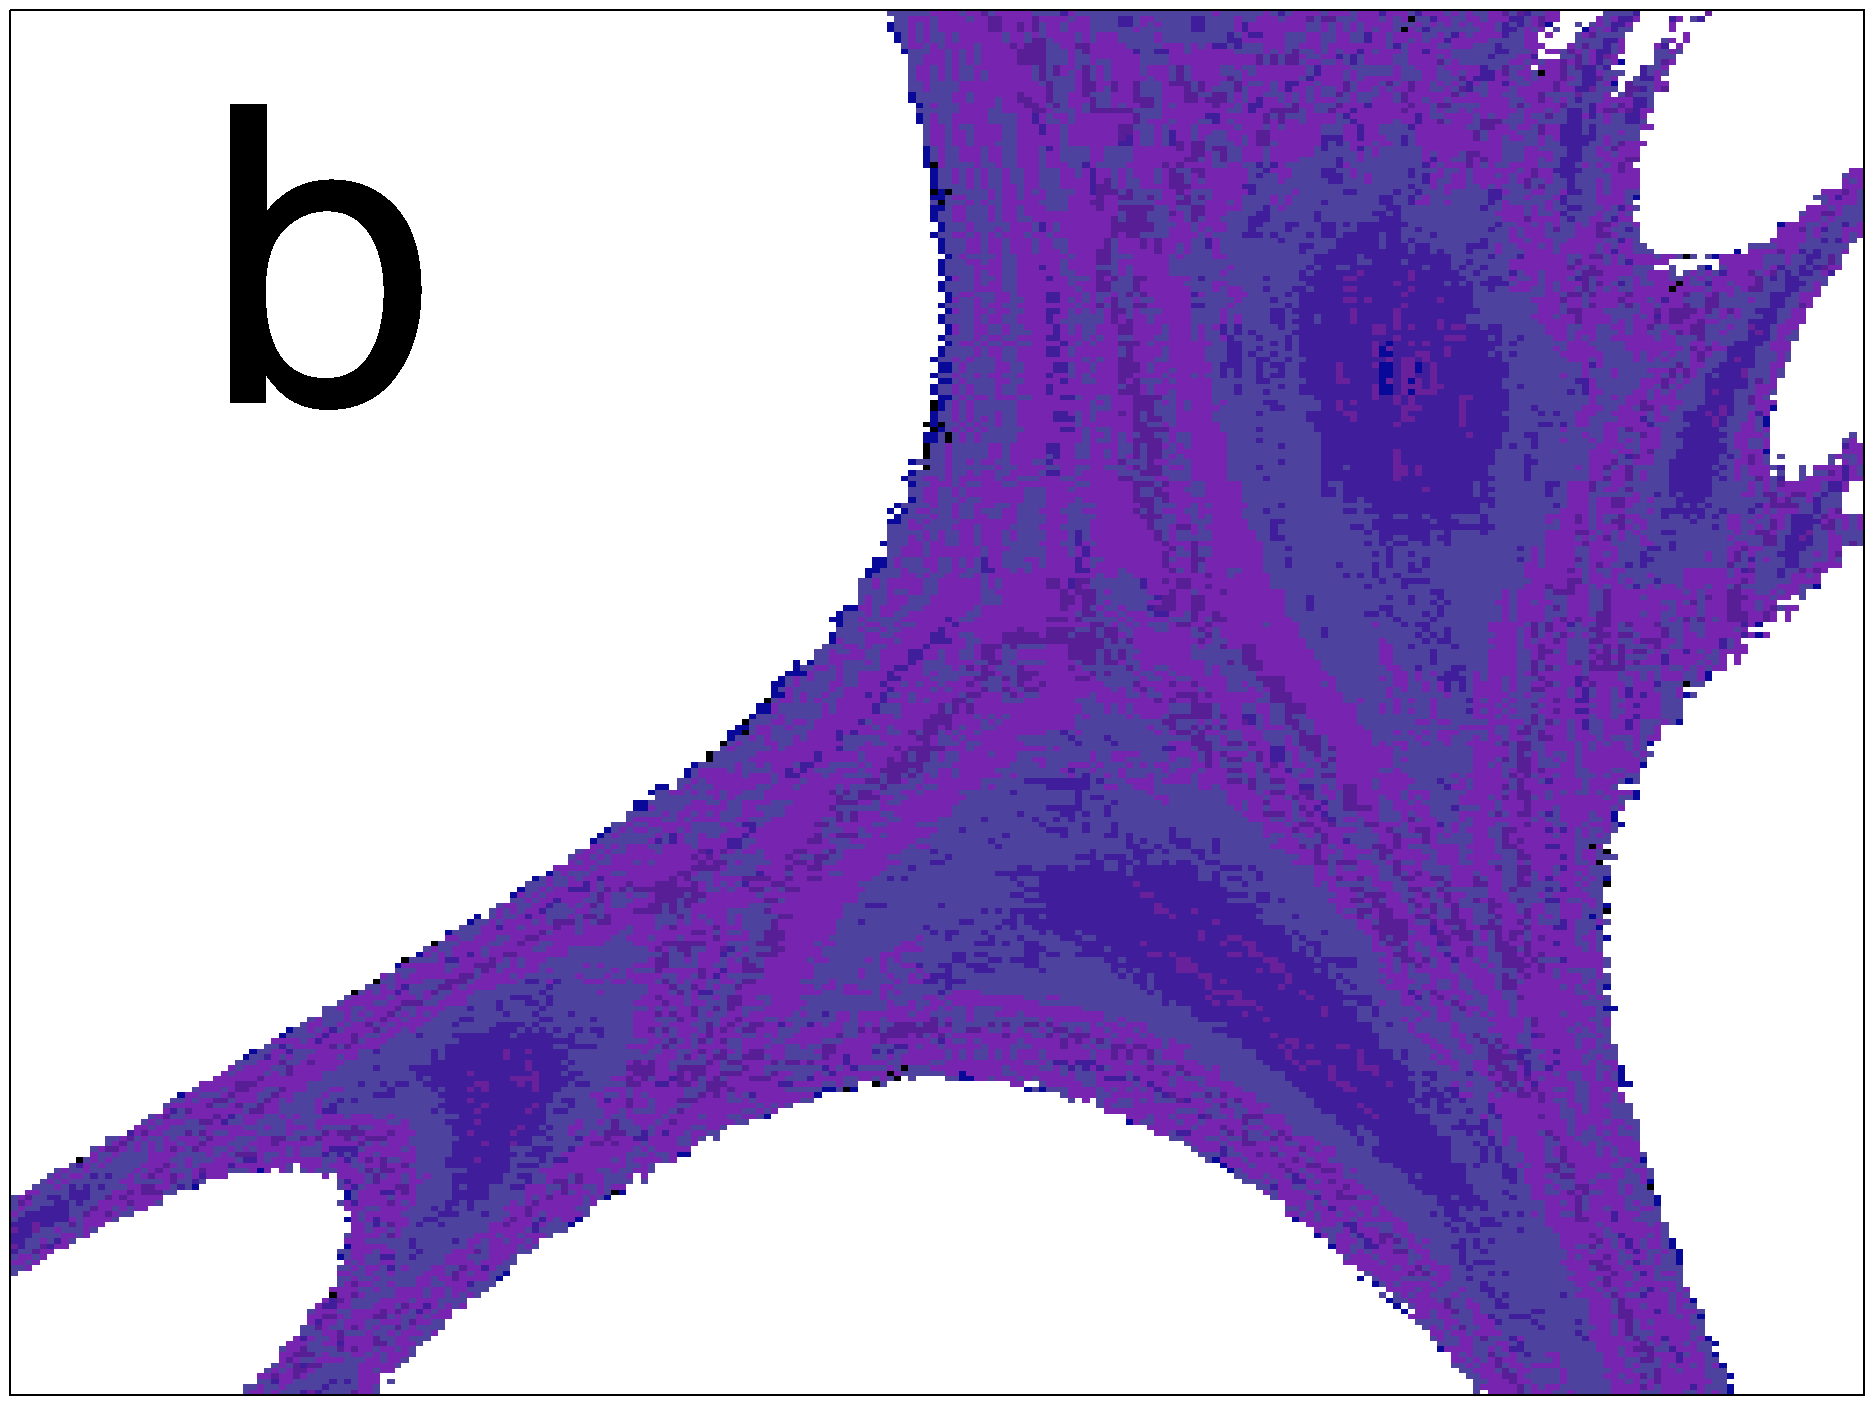
\includegraphics[width=0.3\textwidth]{m6}
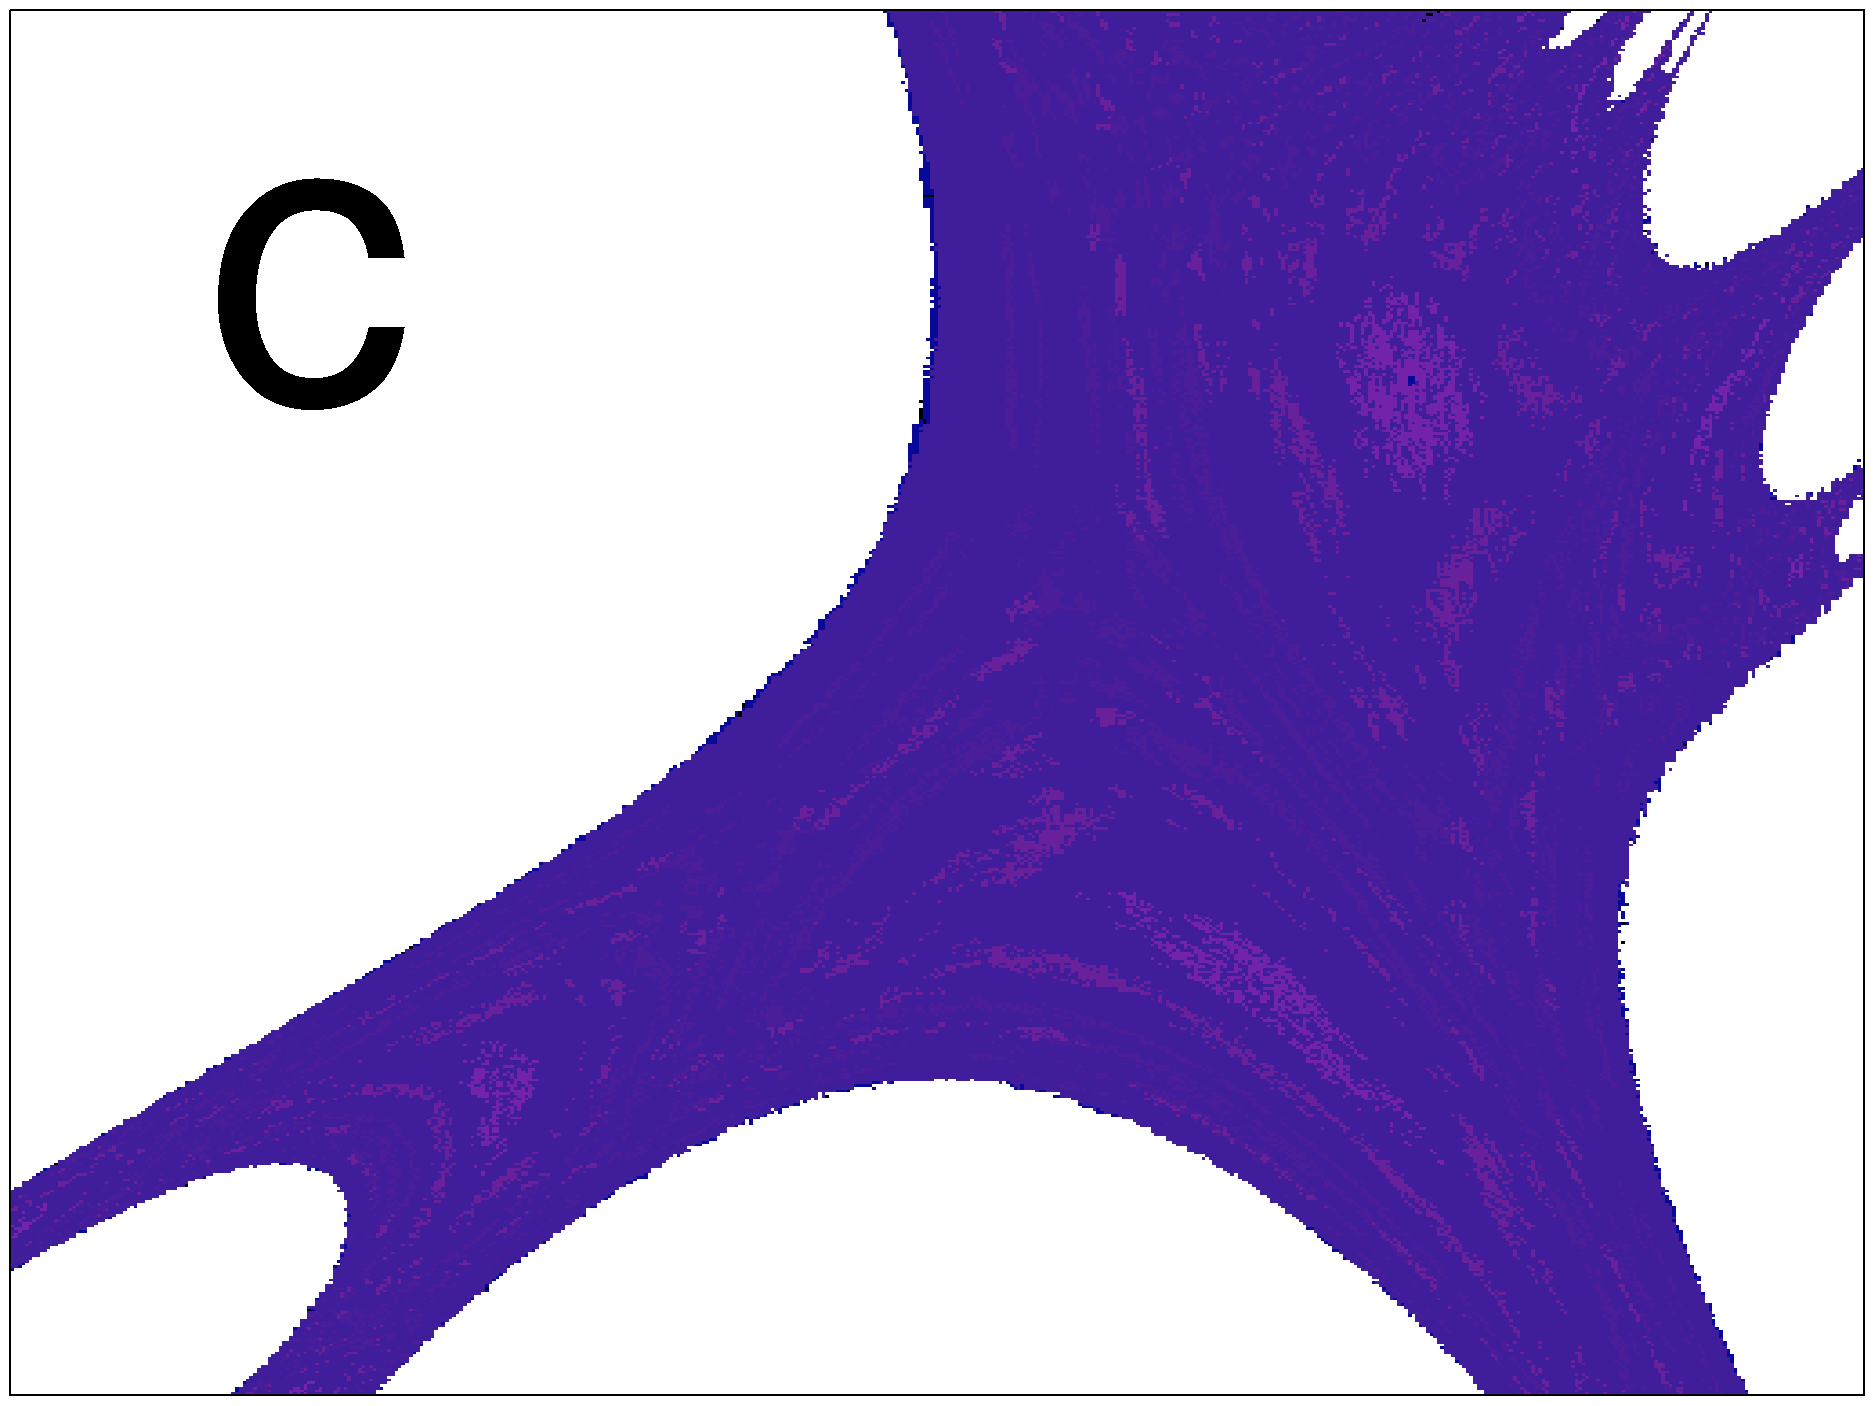
\includegraphics[width=0.3\textwidth]{m7}\\
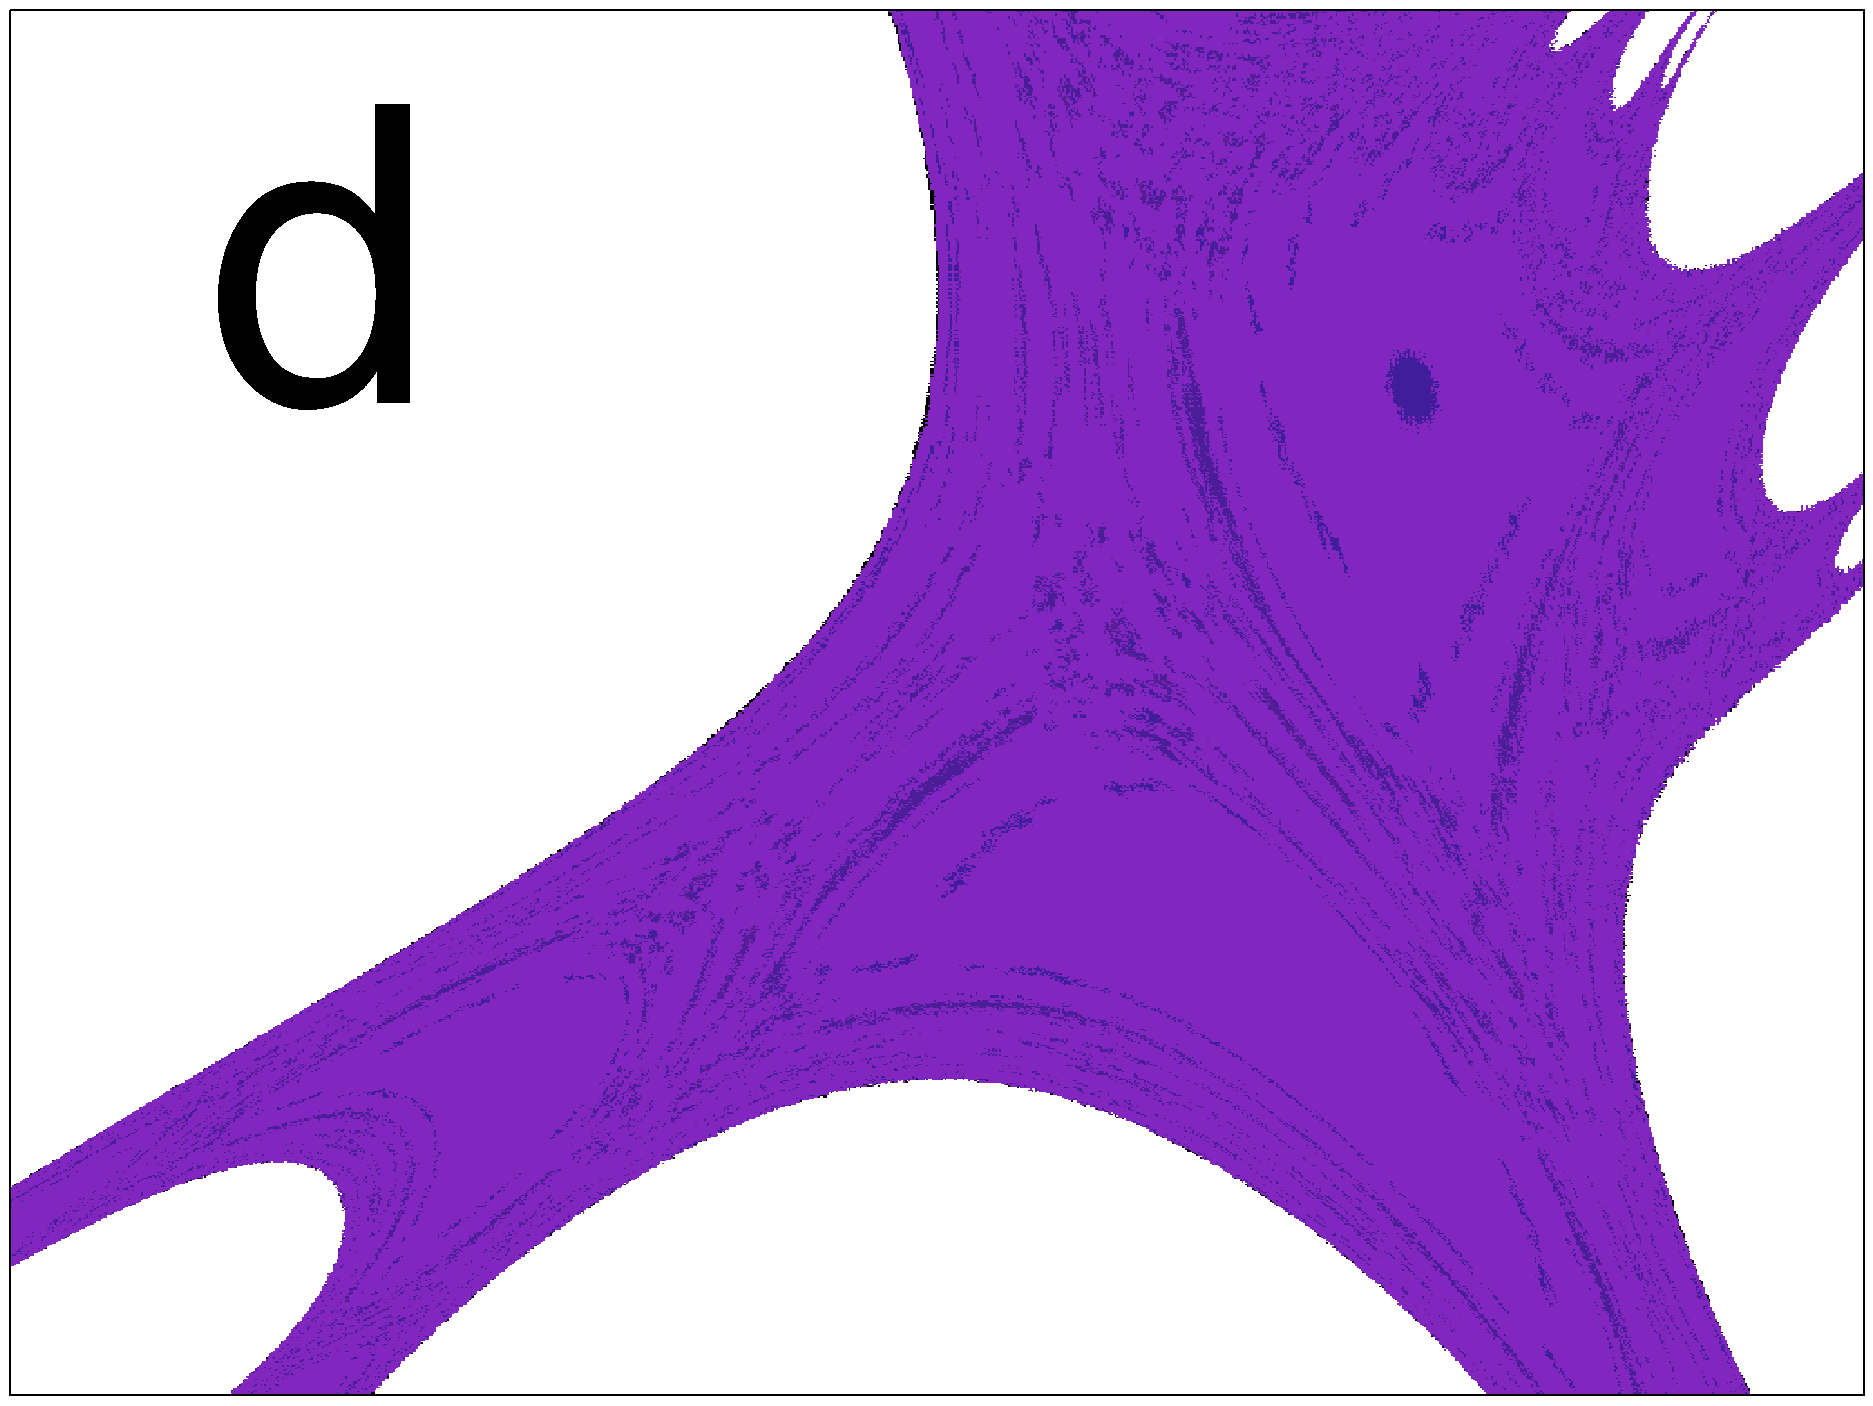
\includegraphics[width=0.3\textwidth]{m8}
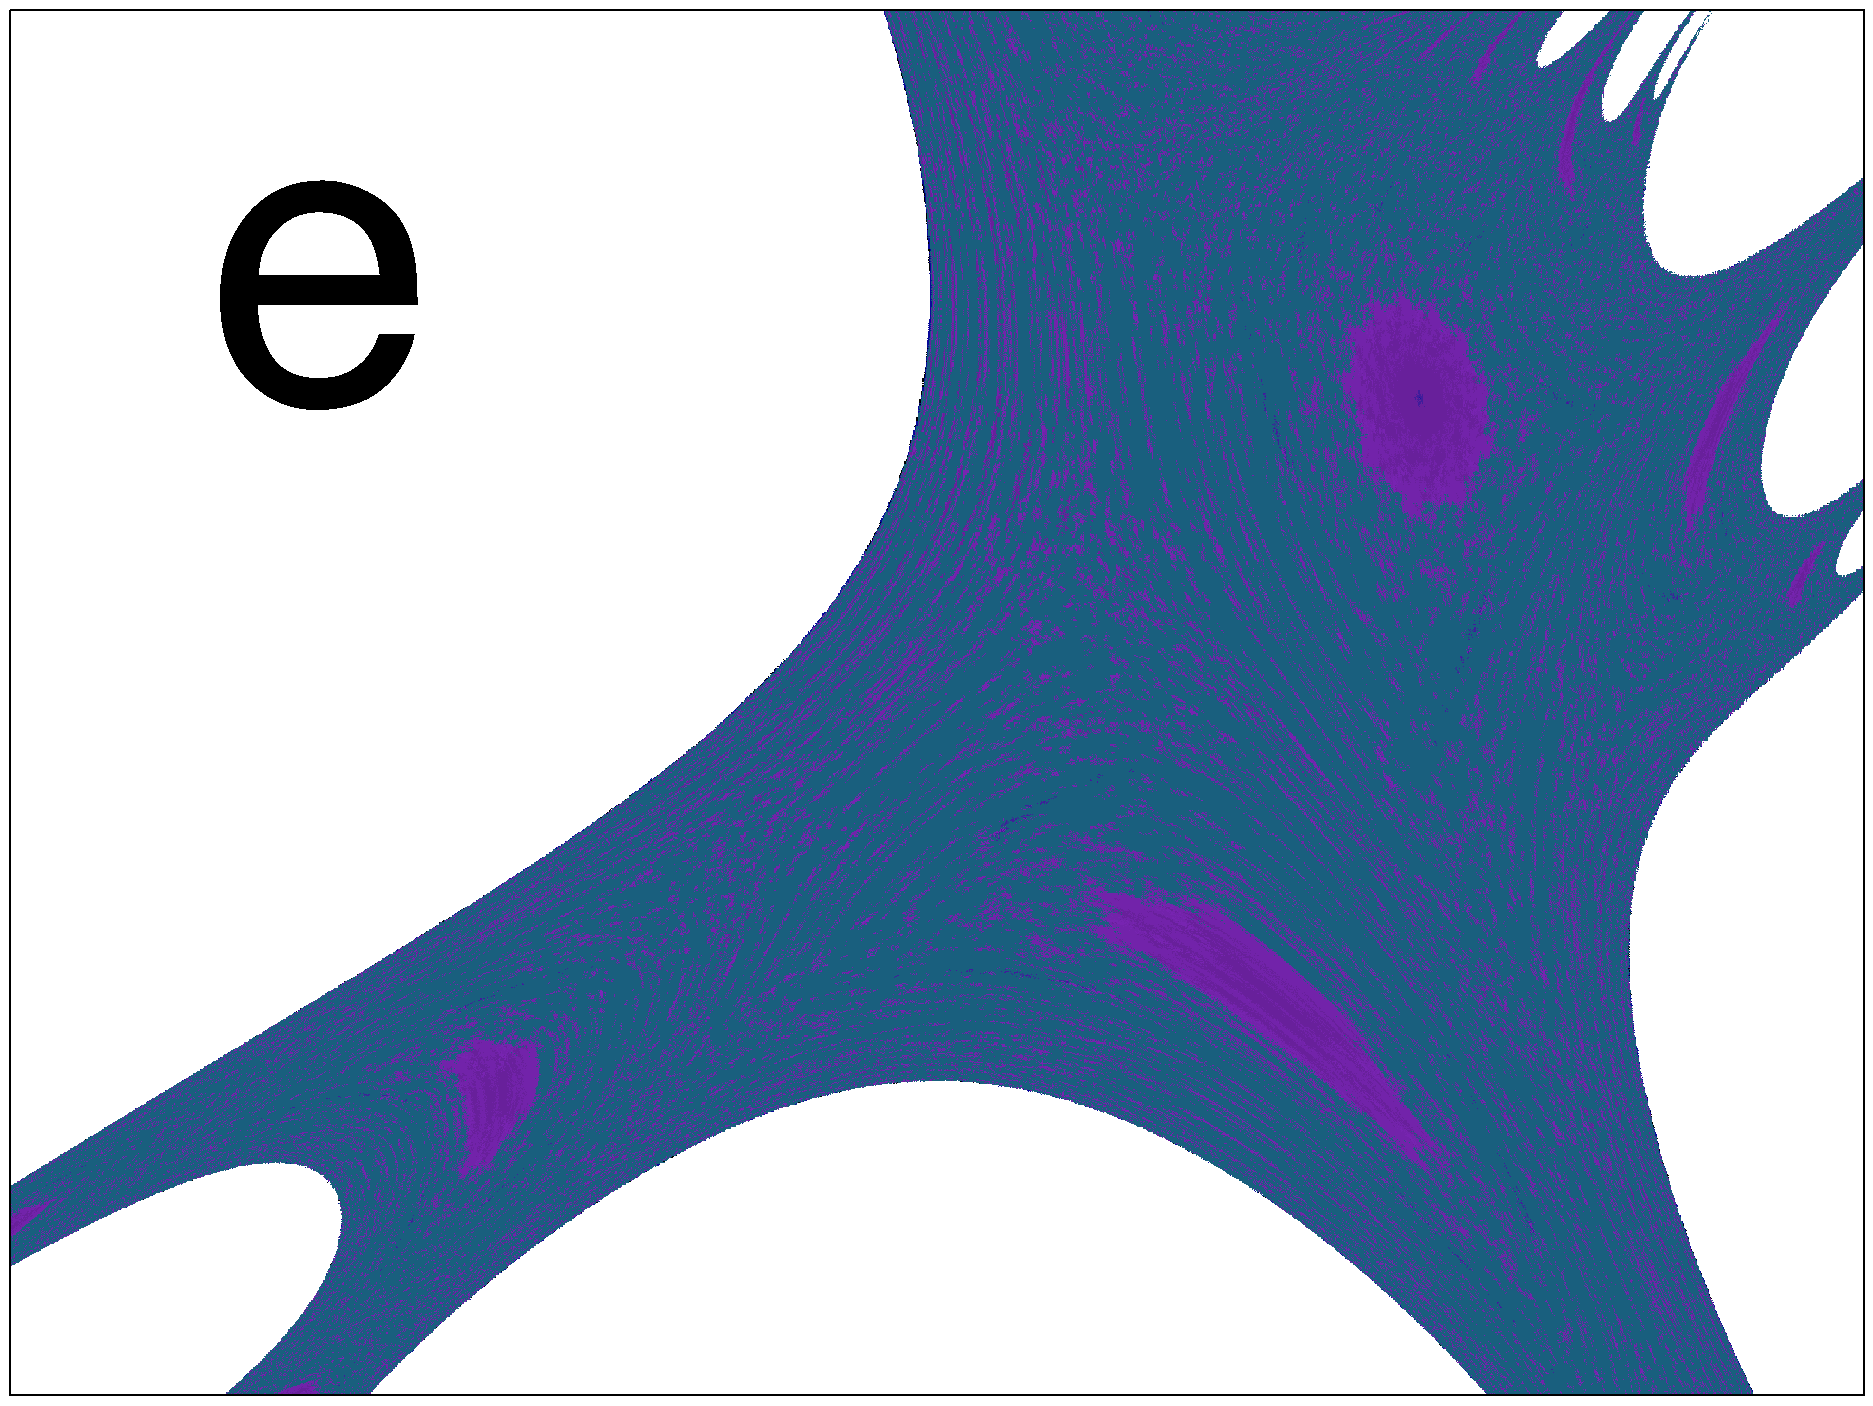
\includegraphics[width=0.3\textwidth]{m9}
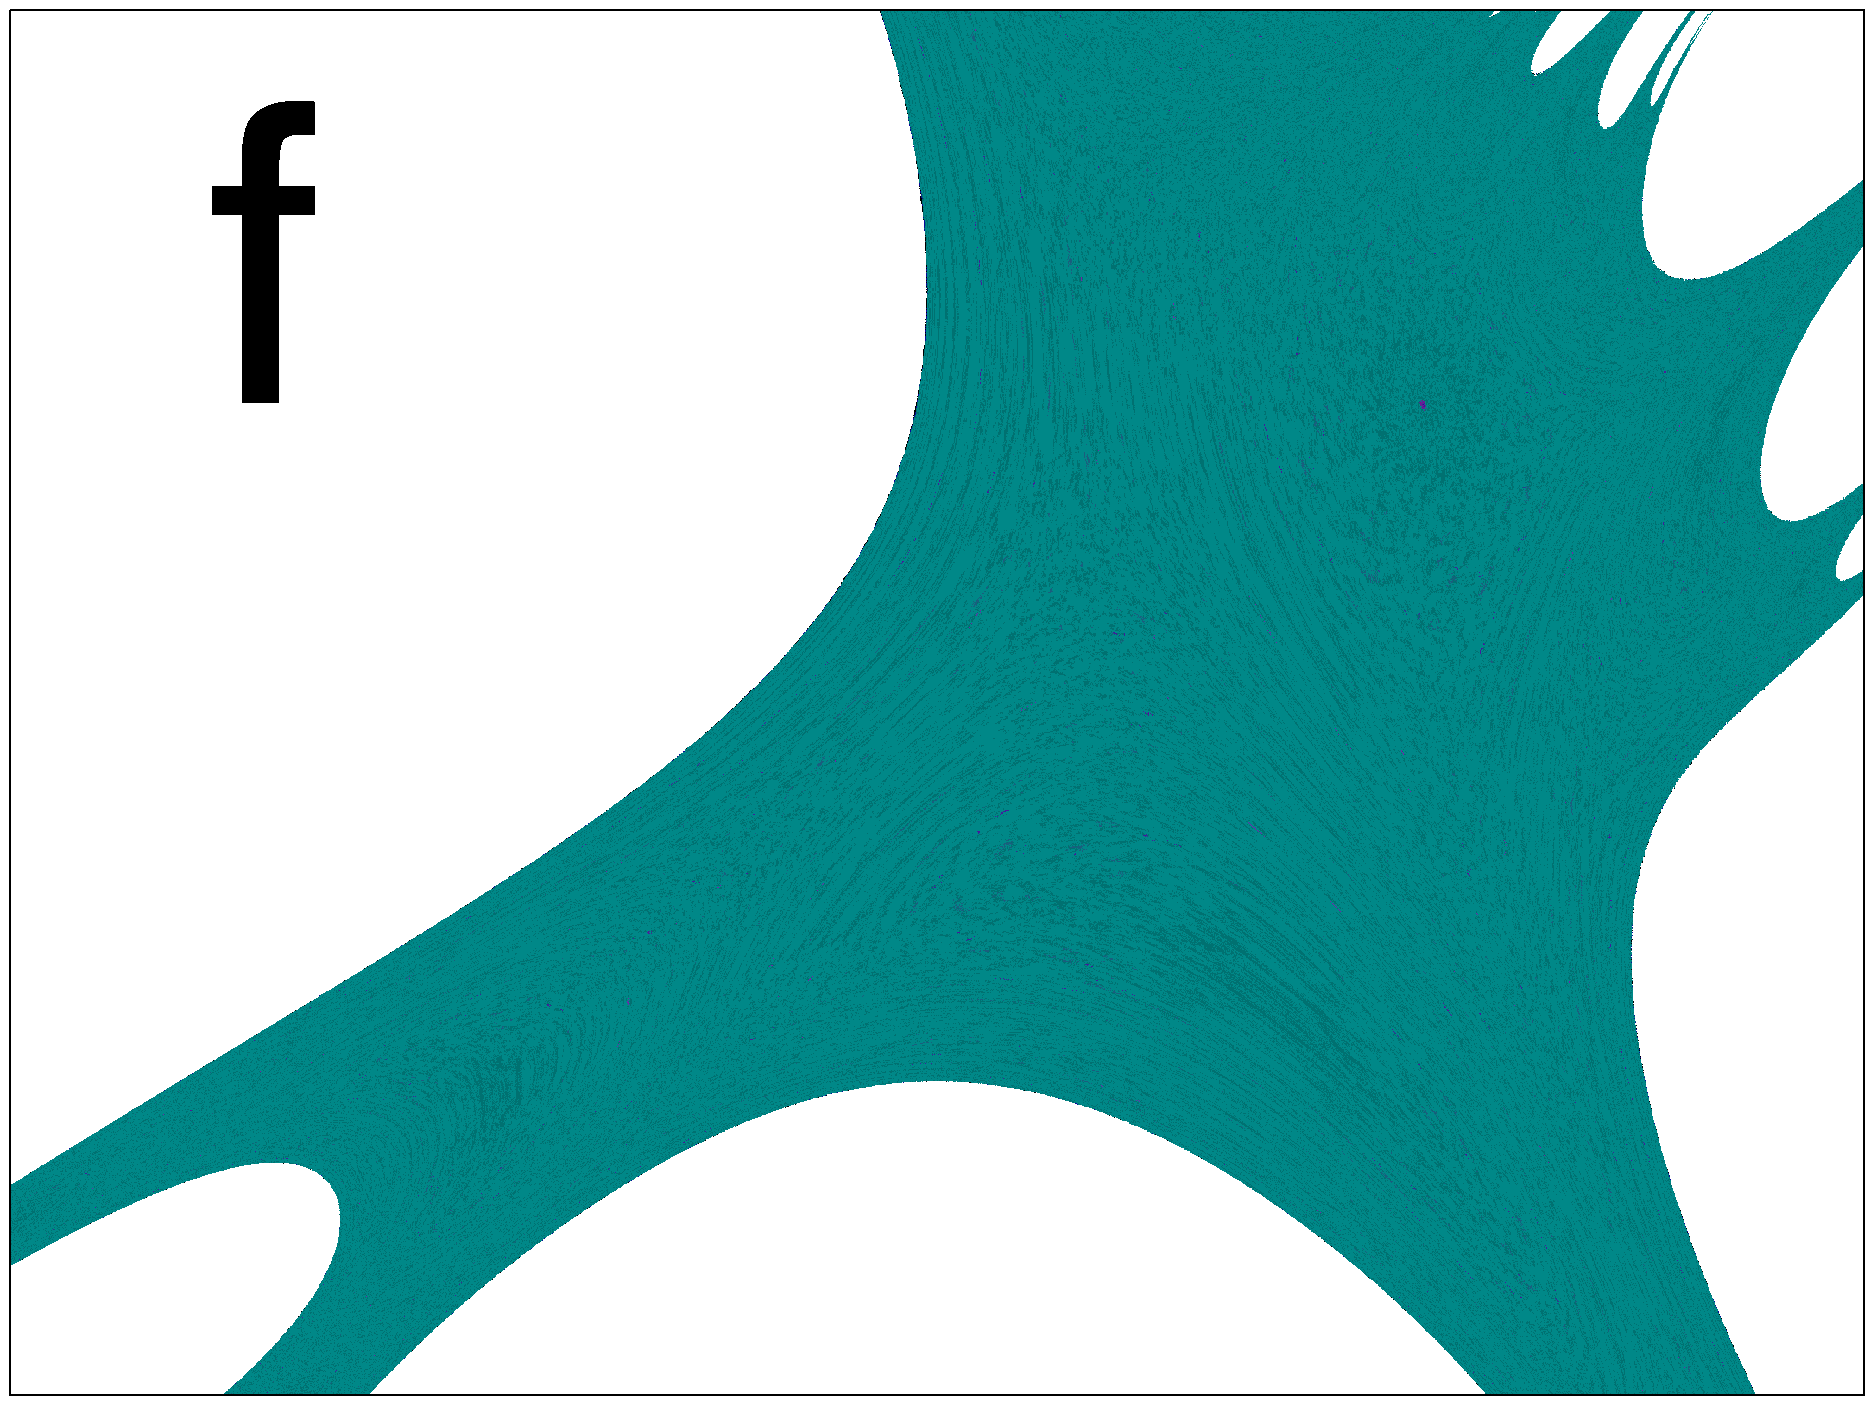
\includegraphics[width=0.3\textwidth]{m10}\\
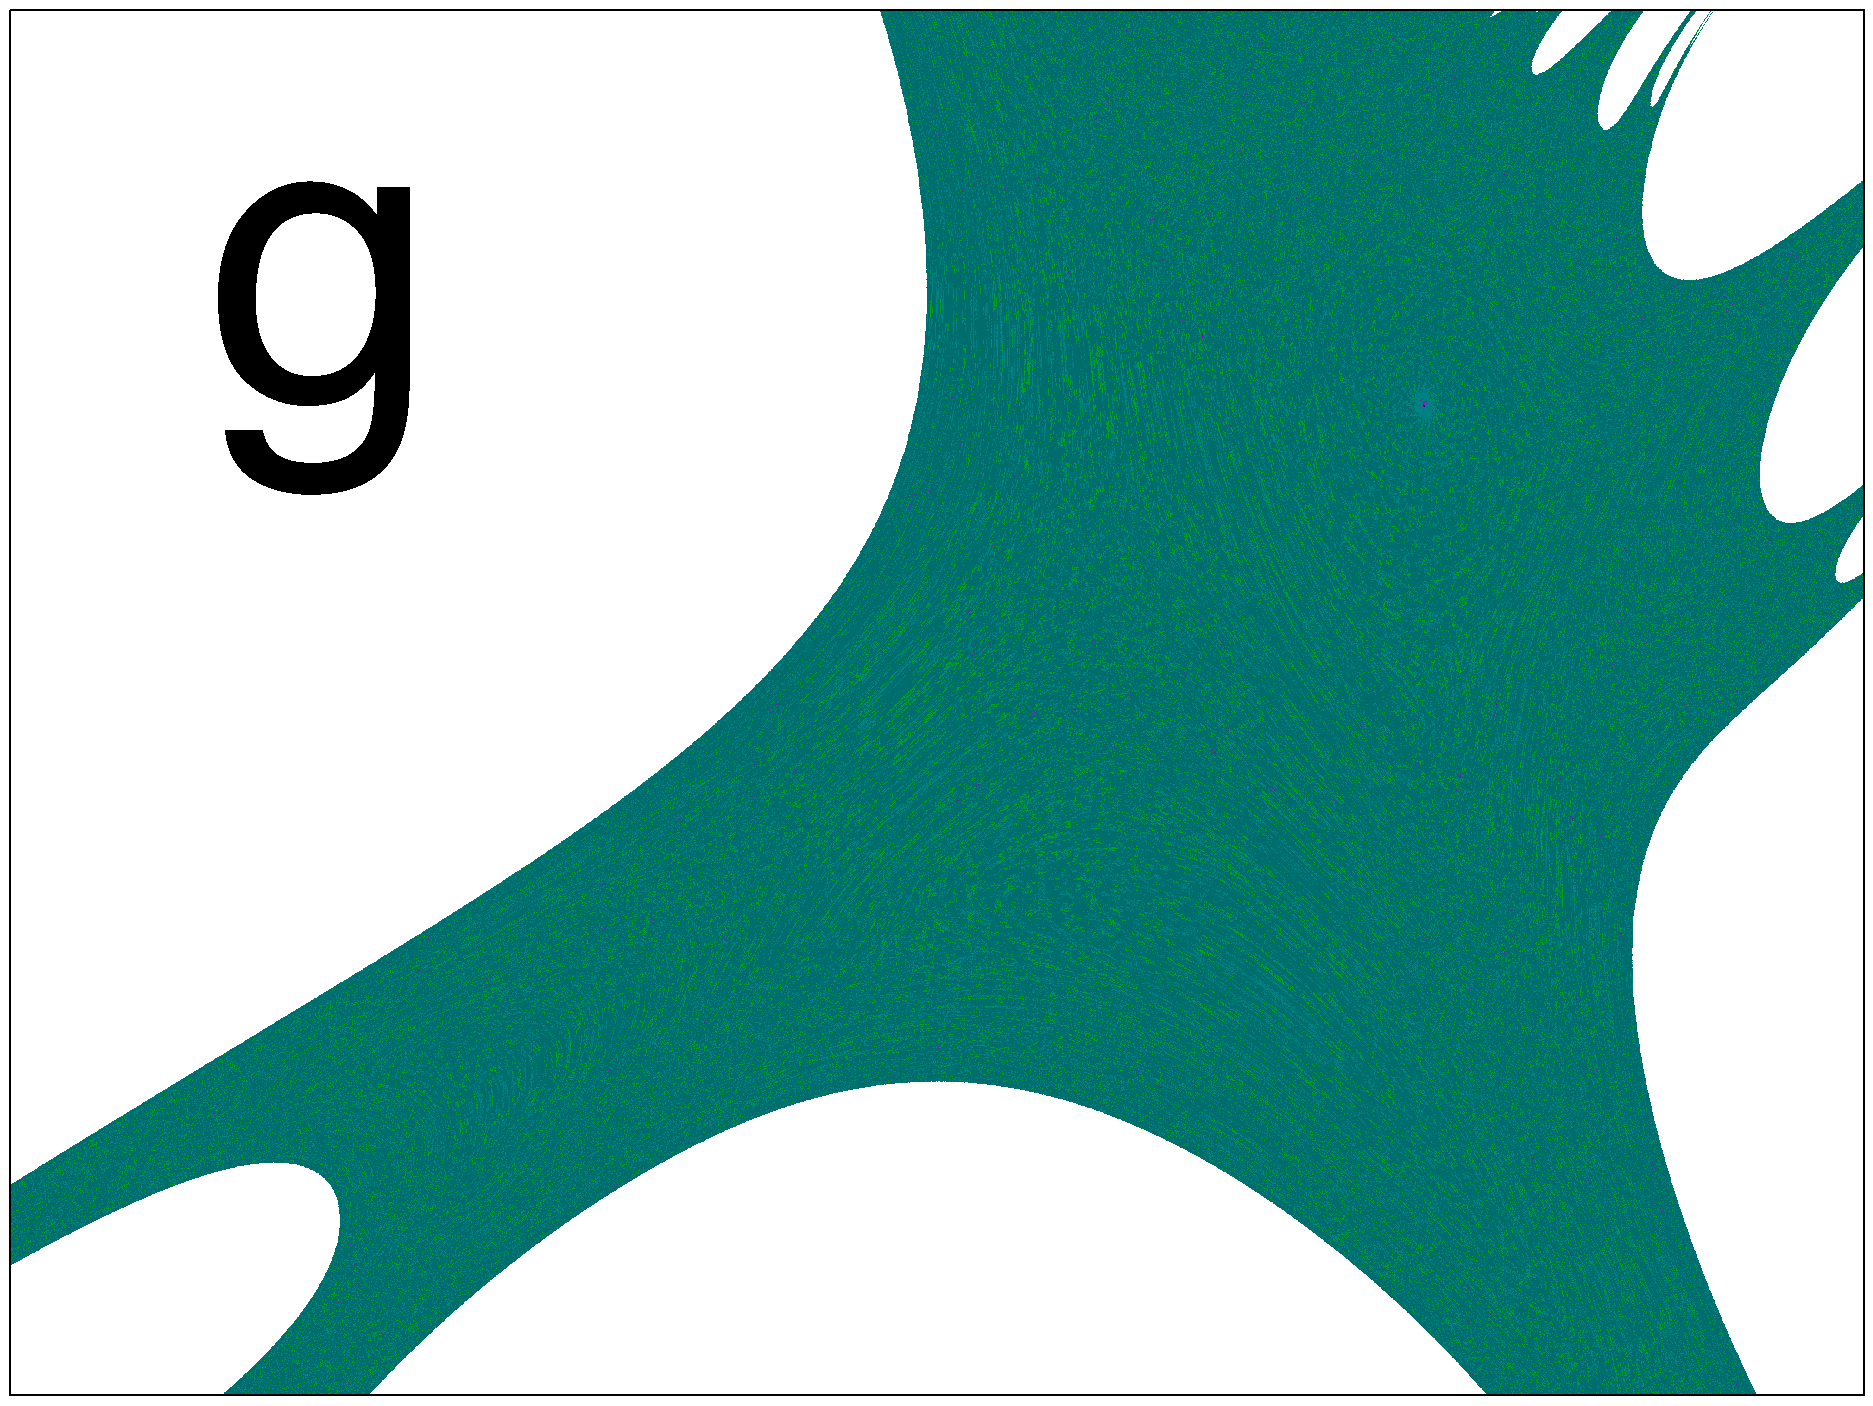
\includegraphics[width=0.3\textwidth]{m11}
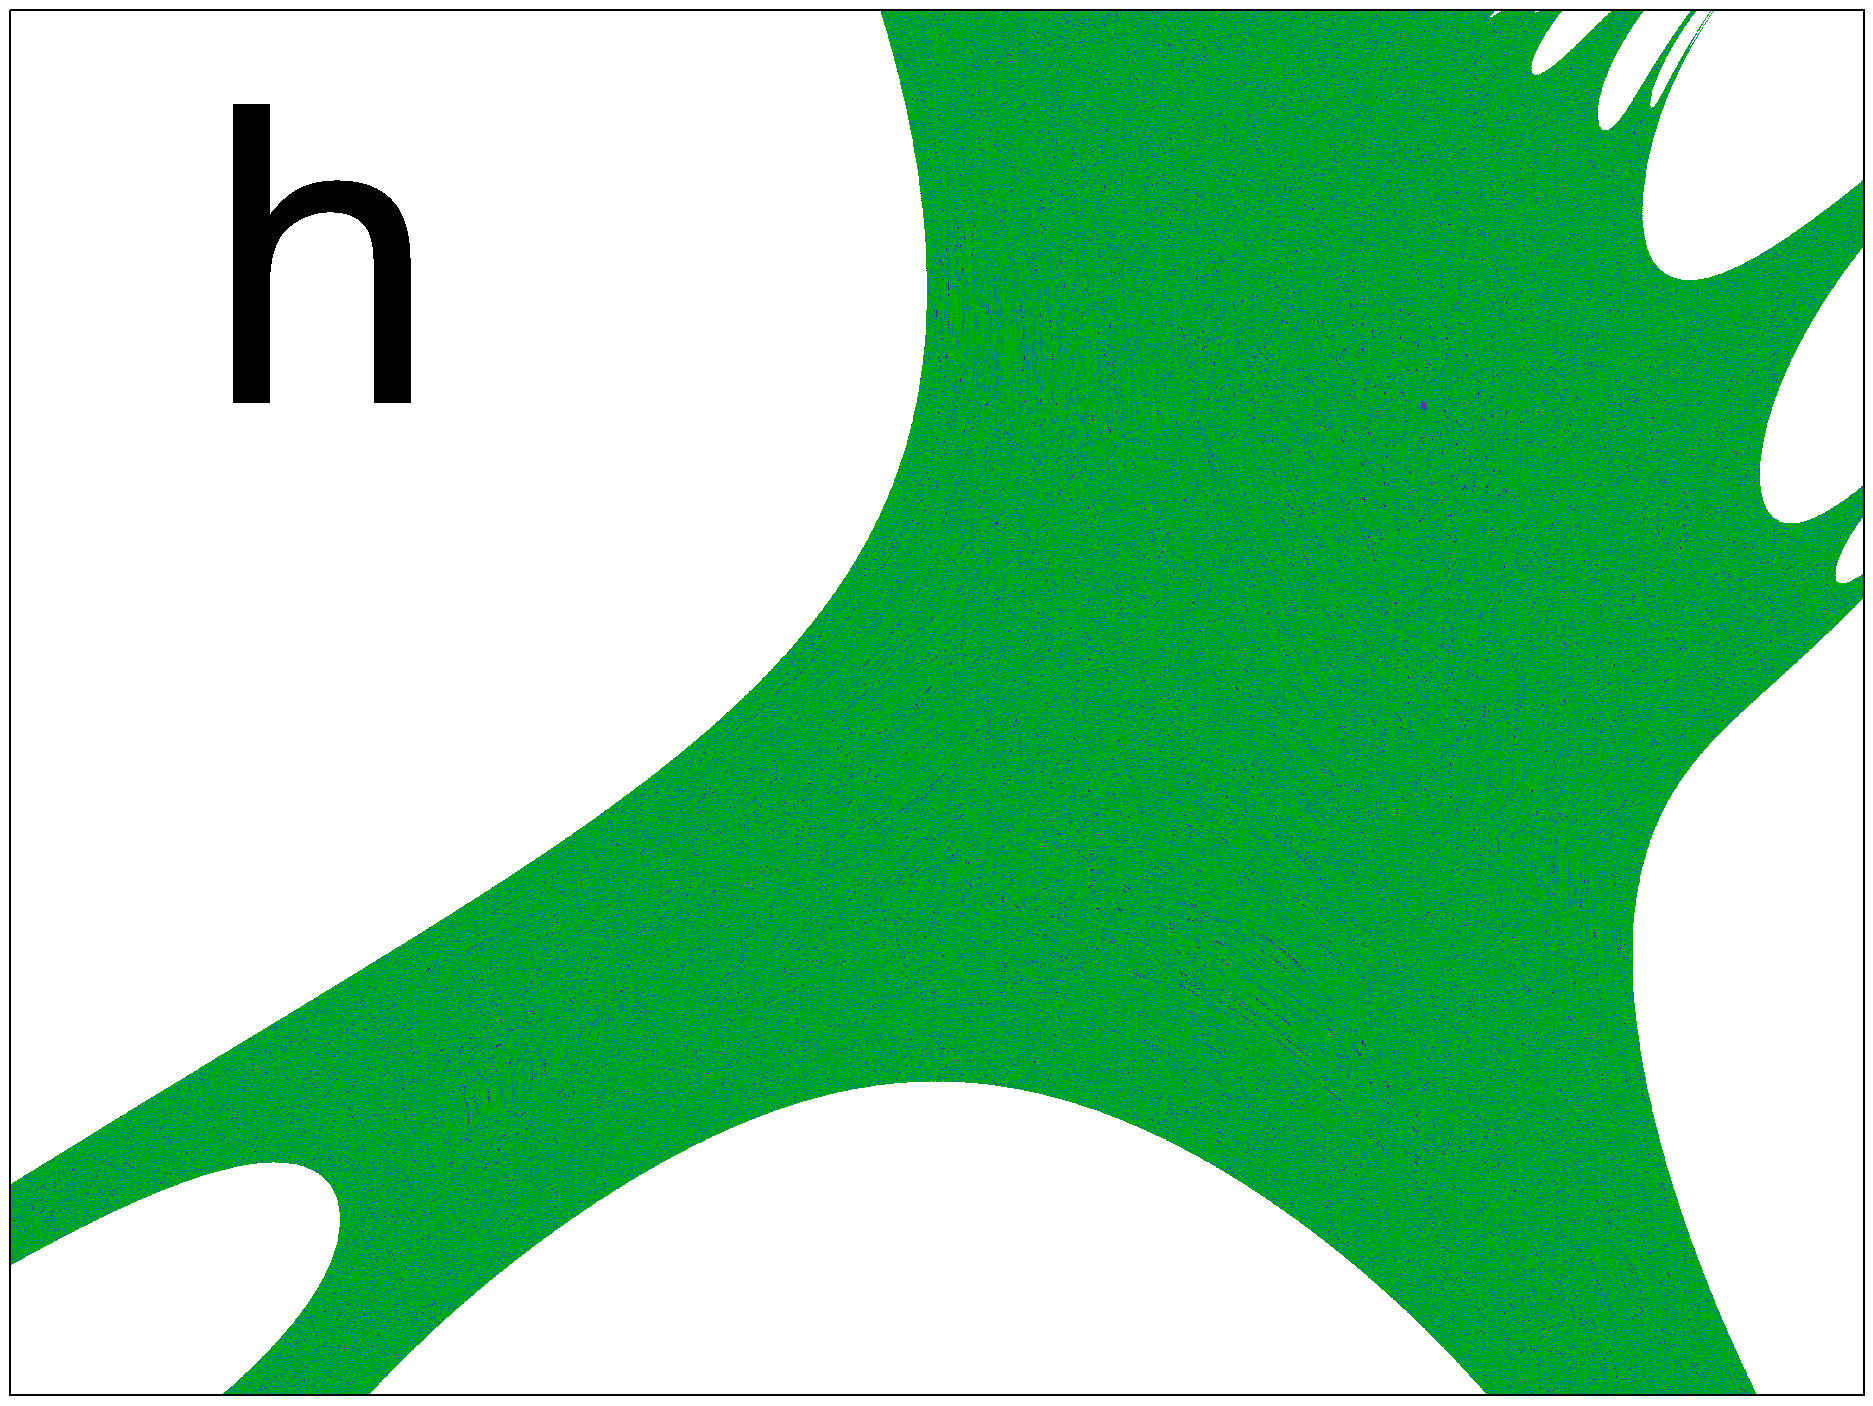
\includegraphics[width=0.3\textwidth]{m12}

\includegraphics[width=0.3\textwidth]{m13}\\

\includegraphics[width=0.3\textwidth]{m14}
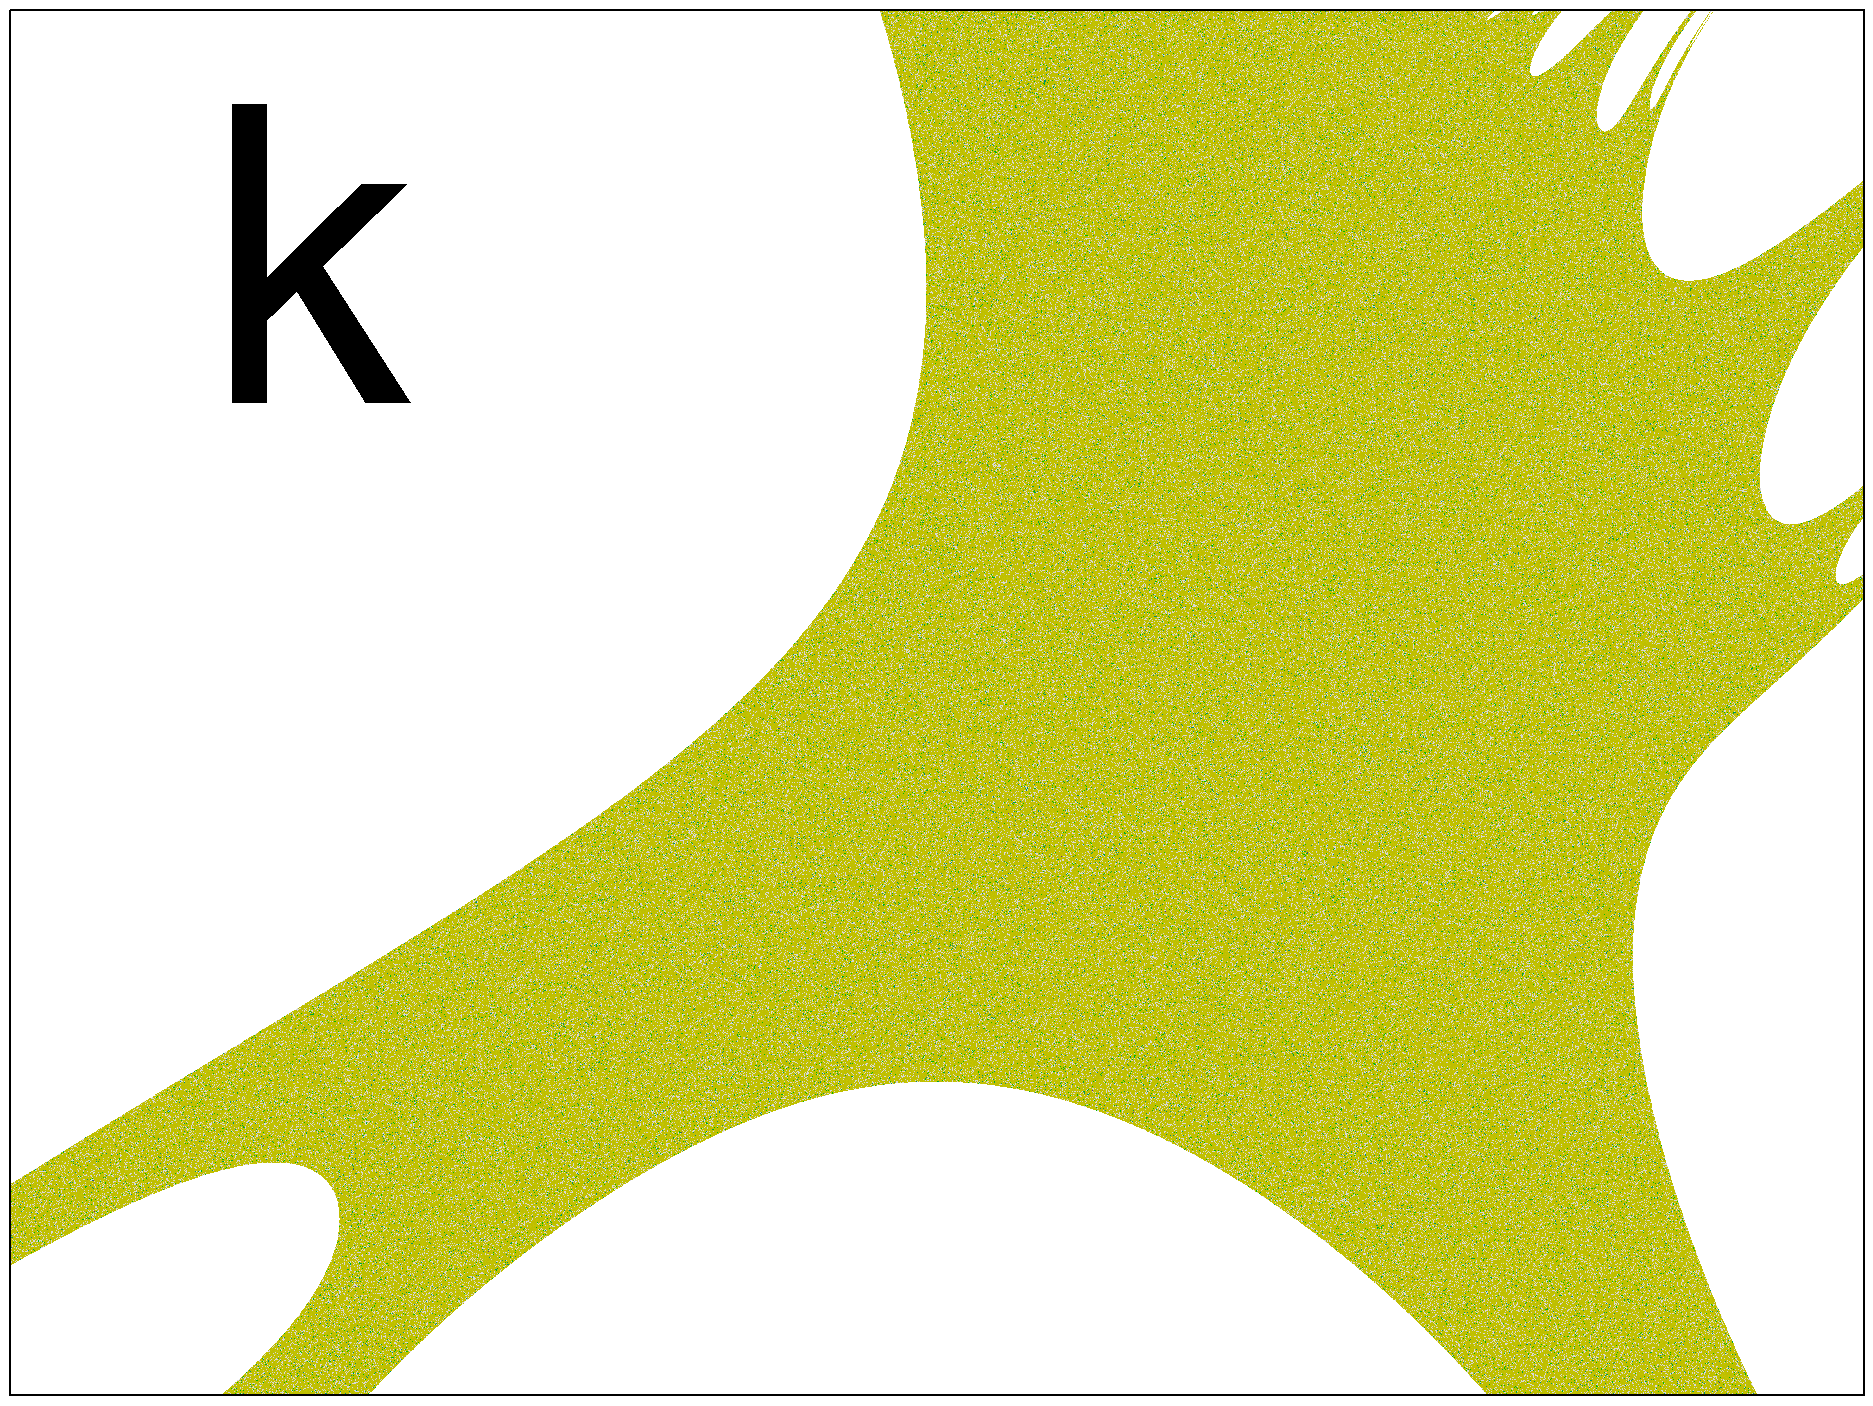
\includegraphics[width=0.3\textwidth]{m17}
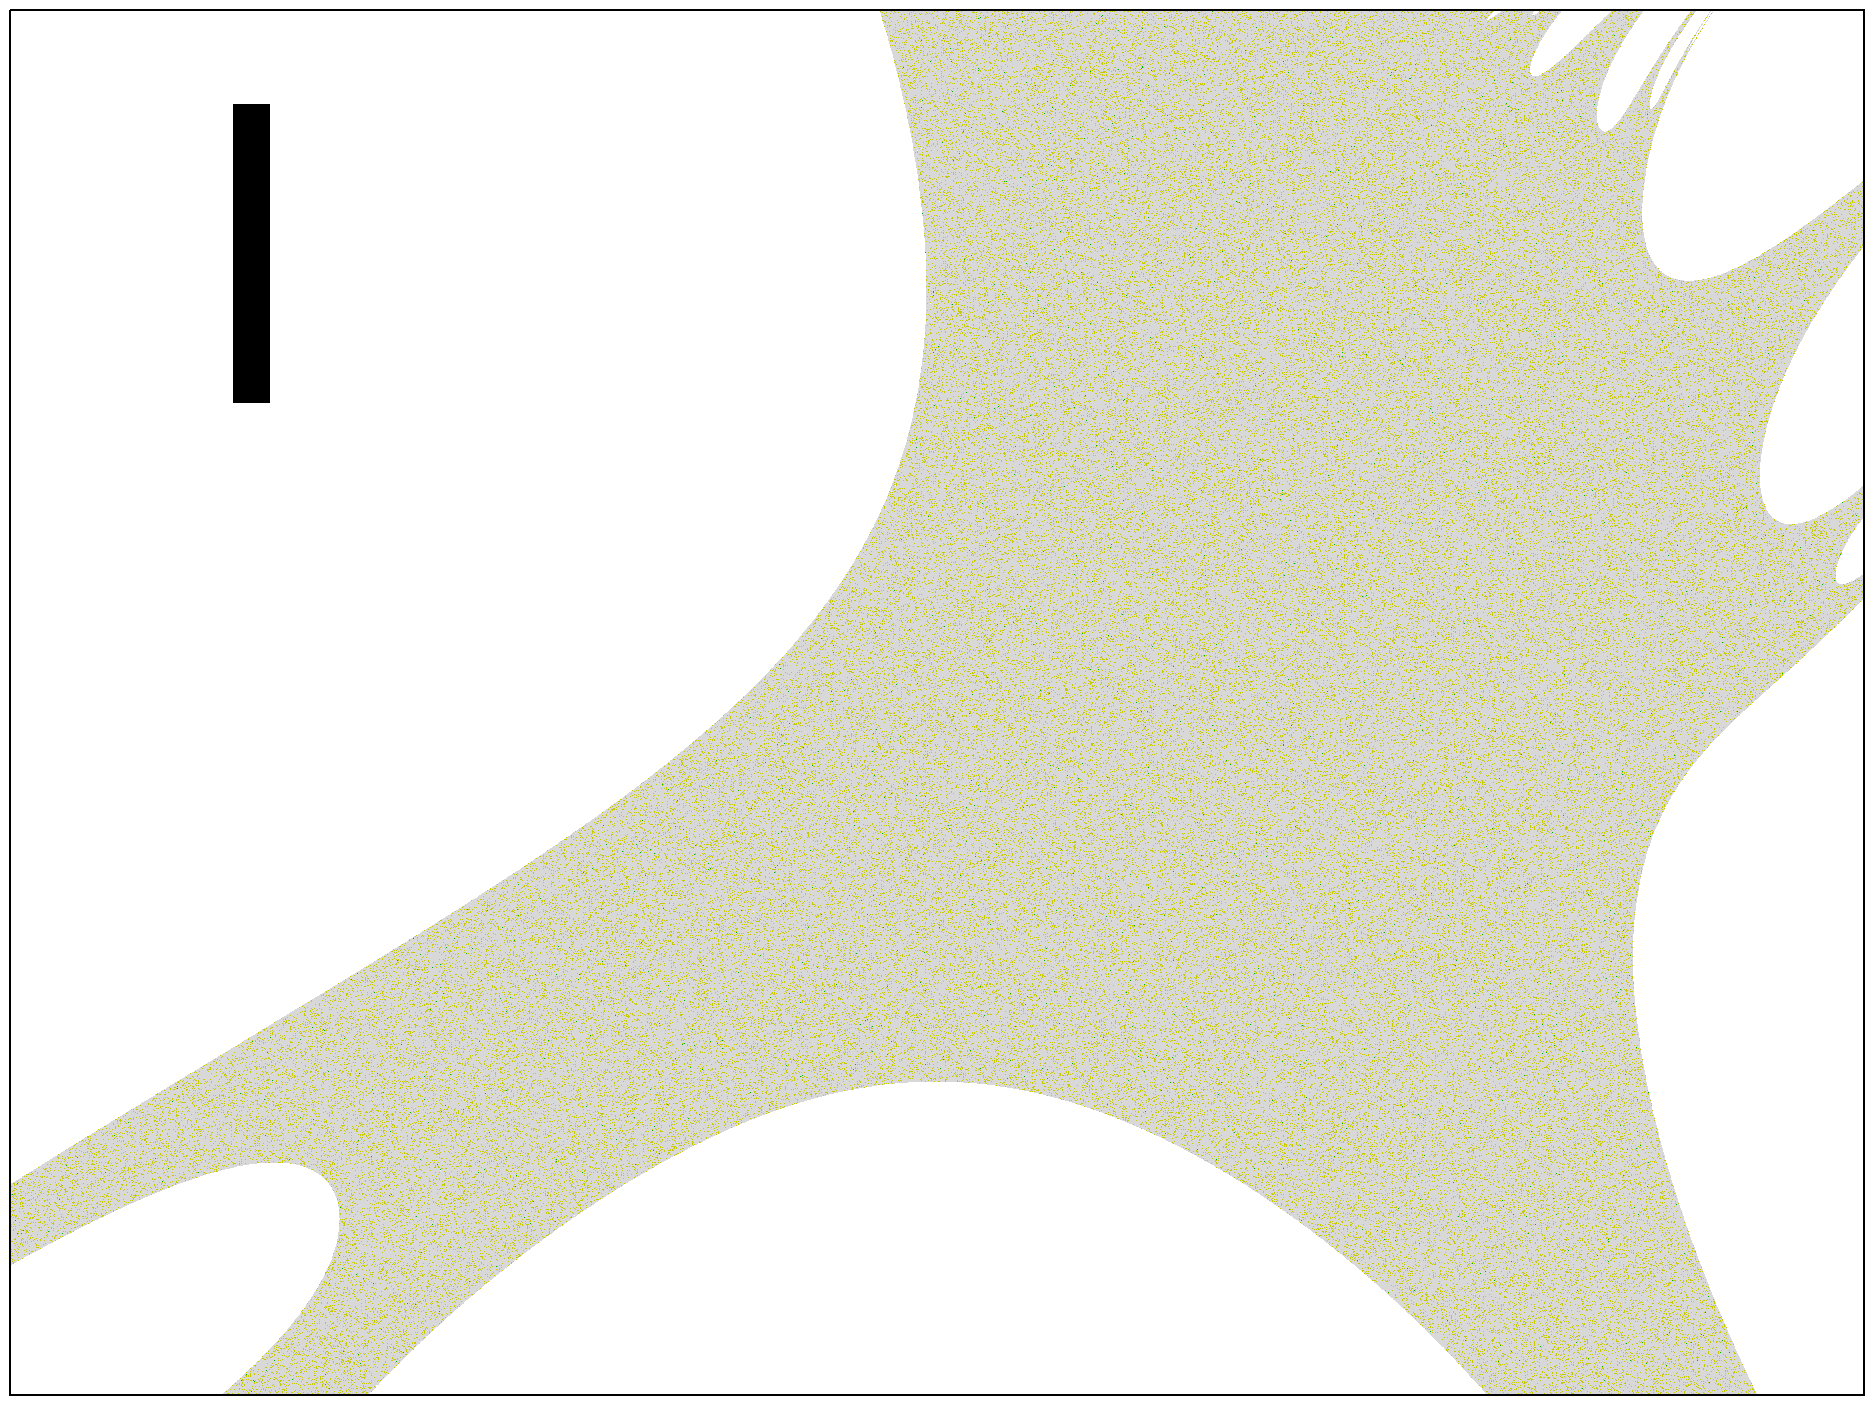
\includegraphics[width=0.3\textwidth]{m18}\\
\\   
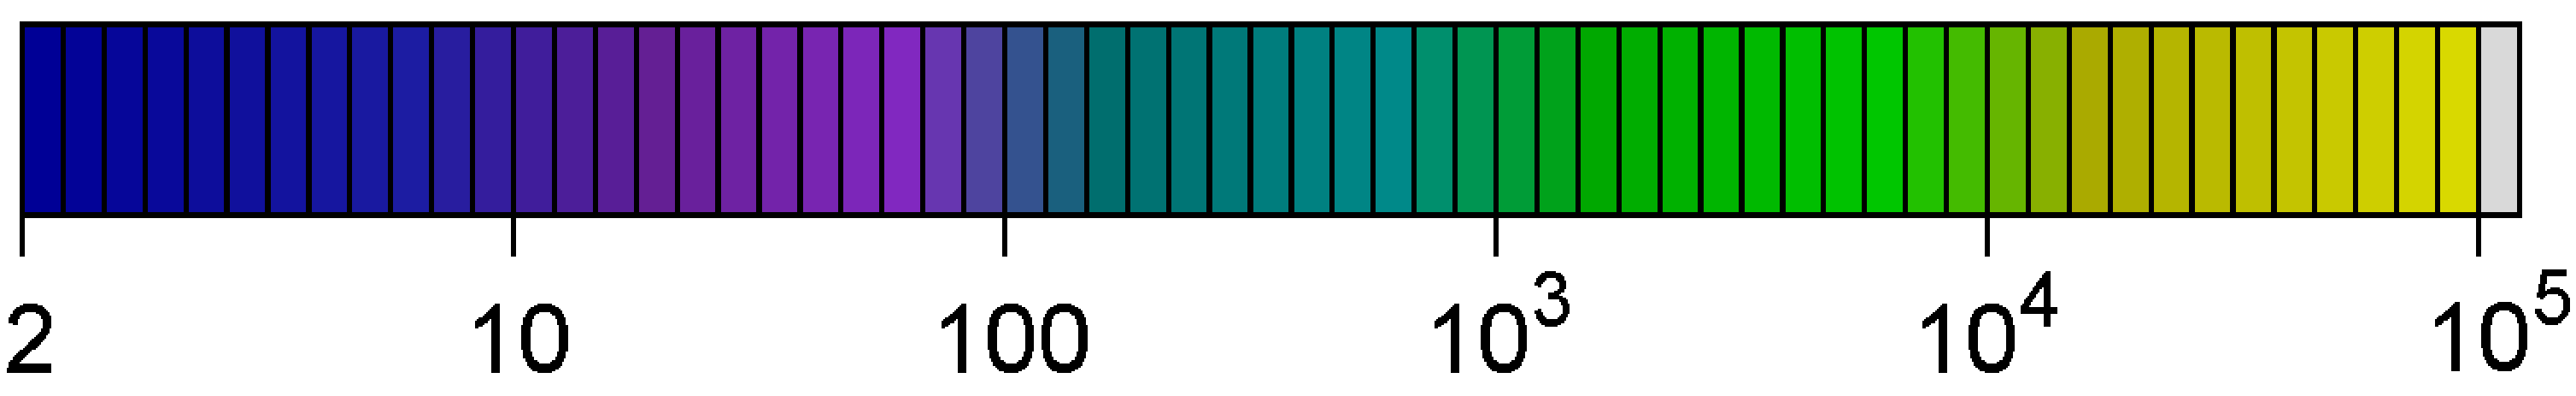
\includegraphics[width=1\textwidth]{ColorMapConEje}
\end{tabular}
\caption{Period's lengths evolution of the attraction domains for: (a) $n_f=5$, (b) $n_f=6$, (c) $n_f=7$, (d) $n_f=8$, (e) $n_f=9$, (f) $n_f=10$, (g) $n_f=11$, (h) $n_f=12$, (i) $n_f=13$, (j) $n_f=14$, (k) $n_f=17$, (l) $n_f=18$.}
\label{fig:m}
\end{figure}

Fig. \ref{fig:m} shows that as the value of $n_f$ increases the colour of the areas smooth and tend to become lighter, indicating that the CIs converge to
higher periods cycles. This is, the range of initial values
that generate useful sequences increases for higher values of $n_f$.

This can also be seen in Table \ref{tabla}, where as $n_f$ increases the predominant limit cycle's length increases. In the limit, when using floating-point architecture, that is the closest arithmetic to real numbers, all the limit cycles are higher than $10^5$, they converge to the chaotic attractor seen in Fig. \ref{fig:atractores3592}.d.

\begin{table}[!t]
% increase table row spacing, adjust to taste
\renewcommand{\arraystretch}{1.3}

\caption{Lengths of the periods within the attractor domain $x$ and $y$ $\epsilon$  $[-2,2]$.}
\label{tabla}
\centering
% Some packages, such as MDW tools, offer better commands for making tables
% than the plain LaTeX2e tabular which is used here.
\fontsize{9}{9}\selectfont
\begin{tabular}{l  l  }
\hline
$n_f$ & $T$ {\scriptsize(Percentage of ICs that converge to this period's length cycle)}  \\
\hline
\hline
$5$ & $2$ {\scriptsize($92.7\%$ )};$6$  {\scriptsize($7.3\% )$}\\
$6$ & $88$ {\scriptsize($41.6 \% )$};$44$ {\scriptsize($36.7 \% )$};$12$ {\scriptsize($13.8\% )$};$16$ {\scriptsize($6.2 \% )$};$2$ {\scriptsize($0.8 \% )$};$24$ {\scriptsize($0.6 \% )$};$26$ {\scriptsize($0.2 \%)$}\\
$7$ &  $12$ {\scriptsize($83.5 \% )$};$14$ {\scriptsize($8.9\% )$};$24$ {\scriptsize($5.2\% )$};$34$ {\scriptsize($1.8 \% )$};$2$ {\scriptsize($0.6\% )$} \\
$8$ & $68$ {\scriptsize($91.7\%)$};$14$ {\scriptsize($6.2\%)$};$12$ {\scriptsize($1.8 \%)$};$17$ {\scriptsize($0.2\% )$};$15$ {\scriptsize($0.1 \%)$}\\ 
$9$ & $140$ {\scriptsize($54.5 \%)$};$123$ {\scriptsize($25.4 \%)$};$34$ {\scriptsize($8.6\%)$};$44$ {\scriptsize($4.3 \%)$};$38$ {\scriptsize($3.9 \%)$};$22$ {\scriptsize($2.9 \%)$};$48$;$2$;$12$;$4$ {\scriptsize($<0.1\%)$}\\
$10$ & $655$ {\scriptsize($78.2\%)$};$212$ {\scriptsize($21.1\%)$};$143$ {\scriptsize($0.5\%)$};$12$ {\scriptsize($0.1\%)$};$2$;$36$;$13$;$20$;$10$;$4$ {\scriptsize($<0.1\%)$}\\
$11$ & $153$ {\scriptsize($78.1\%)$};$461$ {\scriptsize($10.8\% )$};$1381$ {\scriptsize($8.7\%)$};$434$ {\scriptsize($2.3\%)$};$18$;$30$;$53$;$32$;$34$;$10$;$2$ {\scriptsize($<0.1\% )$}\\
$12$ & $2,278$ {\scriptsize($64.4\%)$};$438$ {\scriptsize($22.4\% )$};$598$ {\scriptsize($7.6\% )$};$886$ {\scriptsize($4.7 \%)$};$12$ {\scriptsize($0.7\%)$};$87$;$2$;$42$;$23$;$32$;$10$ {\scriptsize($<0.1\% )$}\\
$13$ & $11,510$ {\scriptsize($ 98.9\%)$};$1052$ {\scriptsize($1 \%)$};$12$;$26$;$2$;$10$ {\scriptsize($<0.1\% )$}\\
$14$ & $21,333$ {\scriptsize($69.2\% )$};$5.804$ {\scriptsize($16.5\%  )$};$4,795$ {\scriptsize($7.9\%  )$};$1,264$ {\scriptsize($5.8 \% )$};$2,429$ {\scriptsize($0.5\% )$}\\ 
& $46$;$23$;$21$;$10$;$12$;$17$ {\scriptsize($<0.1\%  )$}\\ 
$15$ & $10,099$ {\scriptsize($58.6 \%)$};$1.762$ {\scriptsize($19.4 \%)$};$14,887$ {\scriptsize($18.3\%)$};$1,598$ {\scriptsize($3.4\%)$};$750$;$105$;$23$;$14$;$2$;$10$ {\scriptsize($<0.1\%)$}\\
$16$ & $54,718$ {\scriptsize($87.5\% )$};$5,017$ {\scriptsize($4.7\% )$};$>10^5$ {\scriptsize($3.7\% )$};$5,367$ {\scriptsize($2.5\% )$};$703$ {\scriptsize($0.9\% )$}\\
& $1,159$;$1,802$ {\scriptsize($0.2\% )$};$377$;$75$;$10$ {\scriptsize($<0.1\%  )$}\\  
$17$ & $37,812$ {\scriptsize($53.1\% )$};$38,456$ {\scriptsize($24.1\% )$};$>10^5$ {\scriptsize($16.0\%)$};$34,749$ {\scriptsize($3.0\% )$};$3,362$;$718$ {\scriptsize($1.5\%)$}\\
& $3,006$,$5,222$ {\scriptsize($0.1\% )$};$15$ {\scriptsize($<0.1 \%)$}\\  
$18$ & $>10^5$ {\scriptsize($87.4\%)$};$52,069$ {\scriptsize($12.5\% )$};$2,471$ {\scriptsize($0.1\% )$};$146$;$51$ {\scriptsize($<0.1 \%)$}\\
$float$ & $>10^5$ {\scriptsize($100\% )$}\\
\hline

\end{tabular}

\end{table}
\normalsize

In relation to the randomness quantifiers, we realized that the analysis performed up to this point was not
enough to fully describe the changes in the dynamic of a digitalized chaotic system. So we decided to further study the data obtained by employing some statistical quantifiers.

As said, in Fig. \ref{fig:avvelo}.a the two gray zones correspond to the initial conditions that converge to the two coexisting cycles of period two and six respectively. Then this two cycles will have a determined value of $H_{hist}$ and $H_{BP}$, $H_{hist}\mid_{T=2}=0.0625$, $H_{hist}\mid_{T=6}=0.1199$, $H_{BP}\mid_{T=2}=0.1053$ and $H_{BP}\mid_{T=6}=0.2723$. However, the reported value of these quantifiers can not be the average of both, since the frequency of occurrence of cycle two is much greater than that of cycle six (period two appears $92.7\%$ times while period six only $7.3\%$, see Table \ref{tabla}). Therefore, we have calculated the average weighting each quantifier by its frequency of occurrence.\\
Figure \ref{fig:HBPHhist} shows the weighted average of quantifiers $H_{hist}$, $H_{BP}$ and \textsl{MLE}. In the figure it can be seen that the three quantifiers tend to the value calculated using floating-point arithmetic. While $H_{BP}$ and \textsl{MLE} stabilize for $n_f \sim 12$ or $13$, $H_{hist}$ reaches the theoretical value for $n_f \sim 19$, showing that there are properties of the output sequences that only this quantifier can detect.

The $H_{hist}$ - $H_{BP}$ plane, shown in Fig. \ref{fig:HBPvsHhist}, allows a quick visualization of the behavior in terms of randomness of the system, in this plane the ``ideal" pointfrom the point of view of randomness is $(1,1)$. Here, again, the system seems to stabilize for $n_f$ higher than 12. It can be seen that while the $H_{hist}$ stabilizes close to the maximum value ($1$), the $H_{BP}$ tends to $ 0.5$, this value is characteristic of chaotic systems and is due to the structures of their attractors.

A summary of the observed analysis of these outputs can be seen in Fig. \ref{puntos}.

Fig. \ref{puntos}.a and \ref{puntos}.b show the
number of points that diverge and converge to fixed points
respectively as the value of $n_f$ increases, in both cases the
final value tends to the floating-point case. It is clear from
these figures that for $n_f \sim 12$ the system seems have stabilized. Figure
\ref{puntos}.c shows that the averaged period of cycles increases at a logarithmic rate.



%==========================Resumen periodos============================
\begin{figure}
\begin{tabular}{cc}
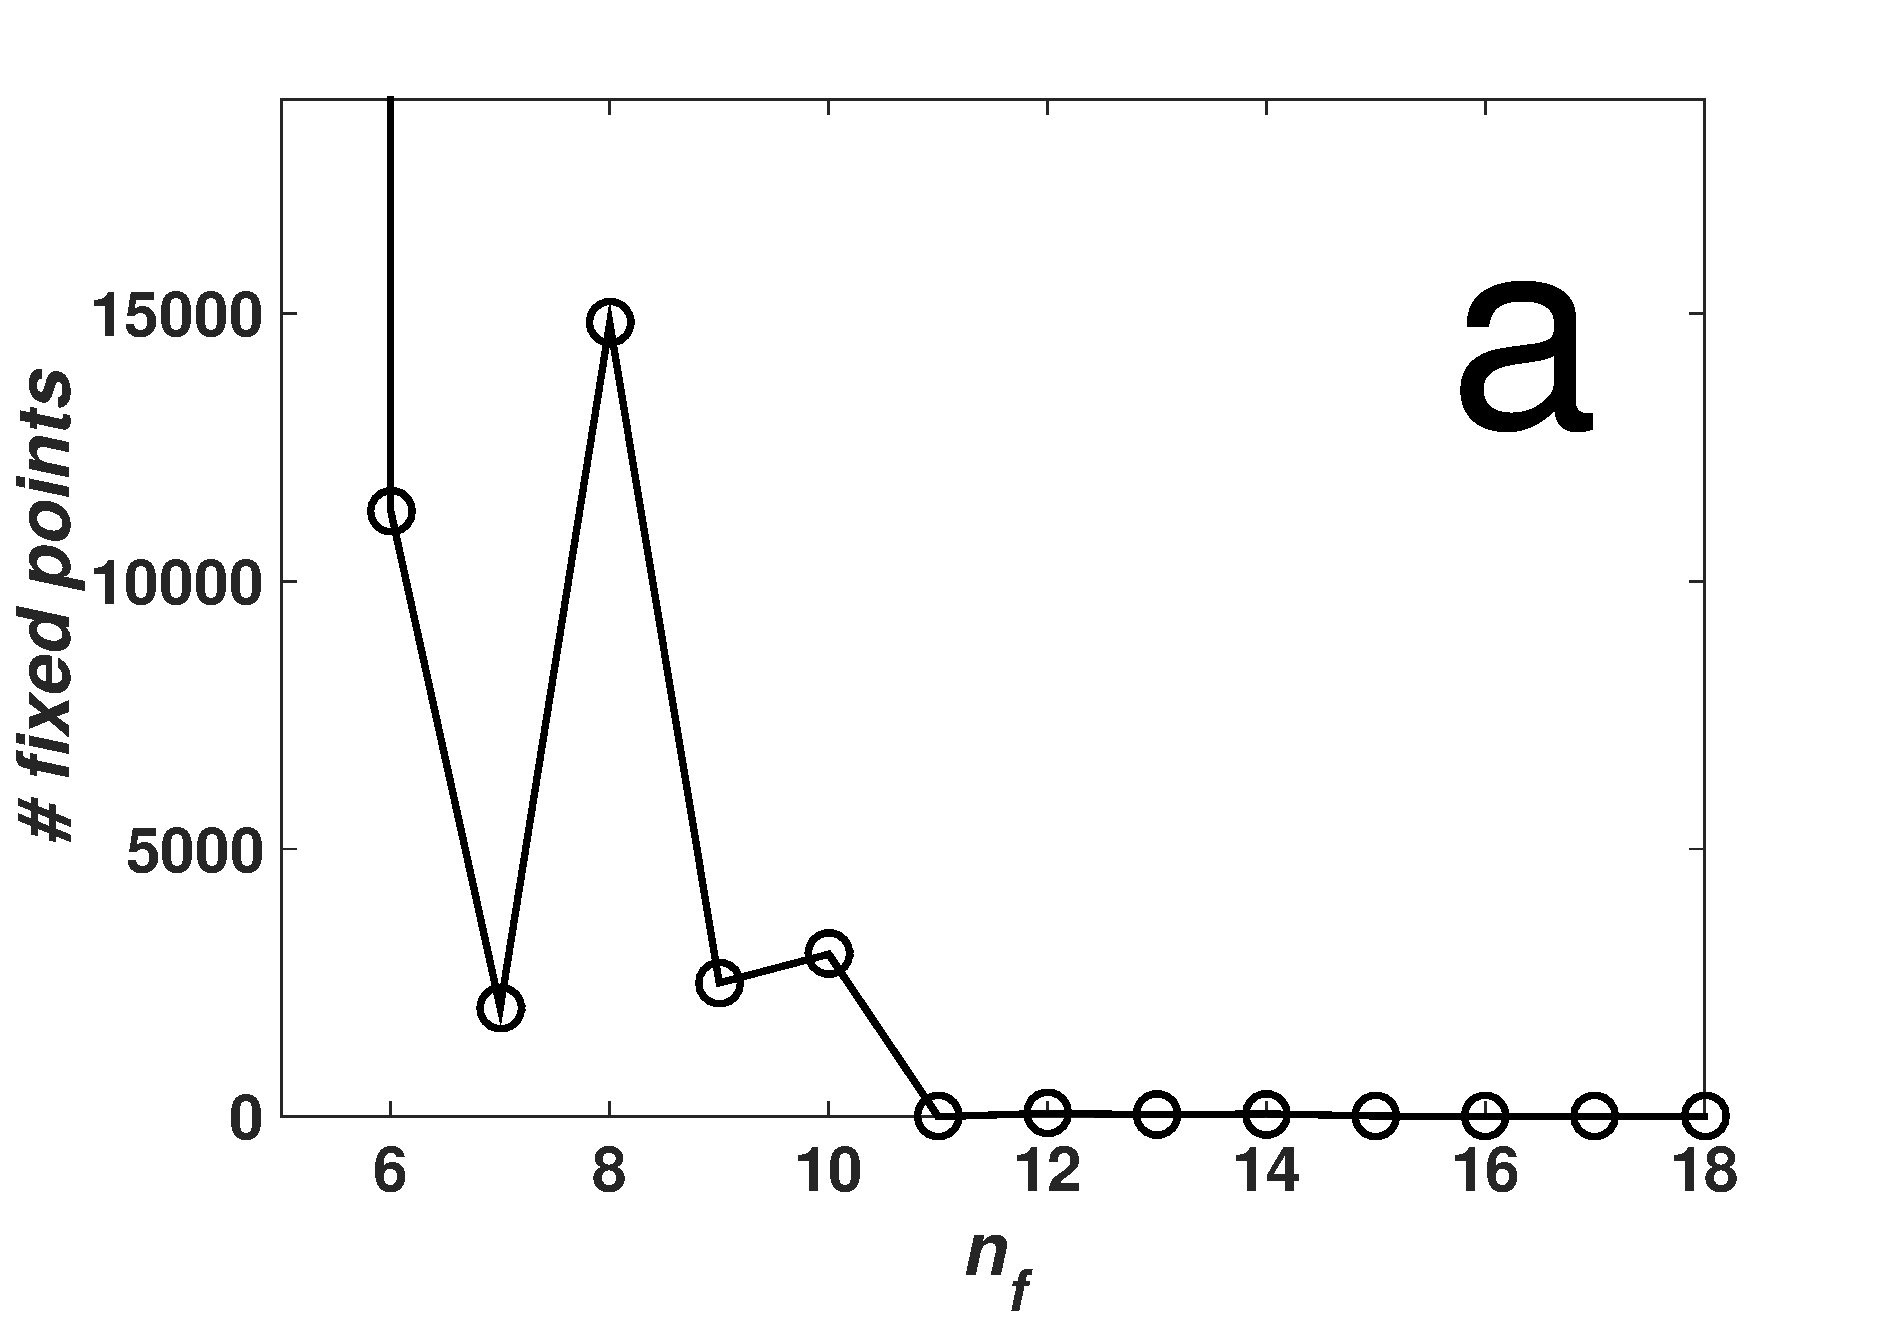
\includegraphics[width=0.48\textwidth]{ptosfijos}
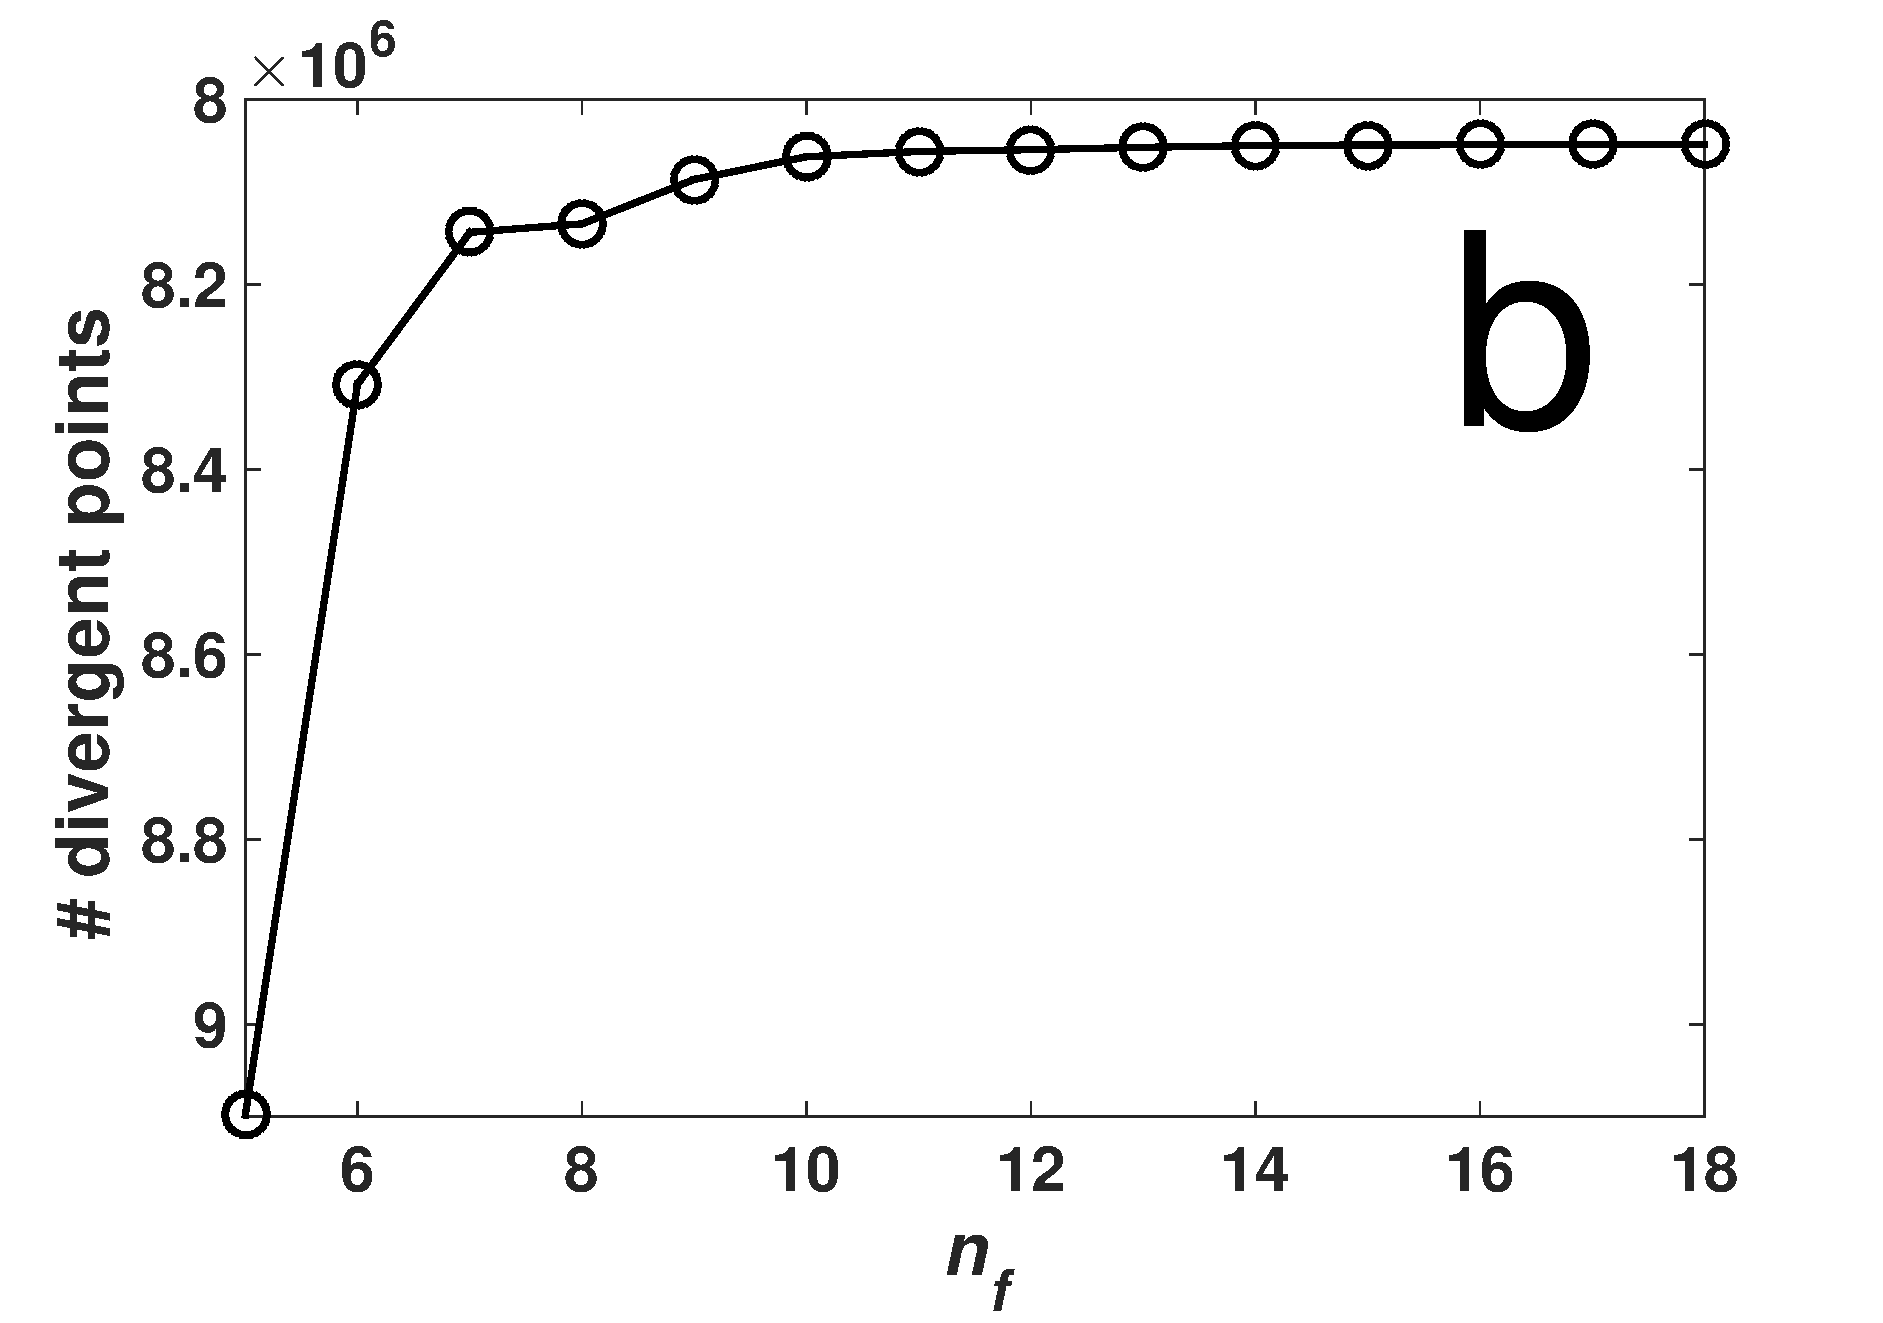
\includegraphics[width=0.48\textwidth]{divergen}\\
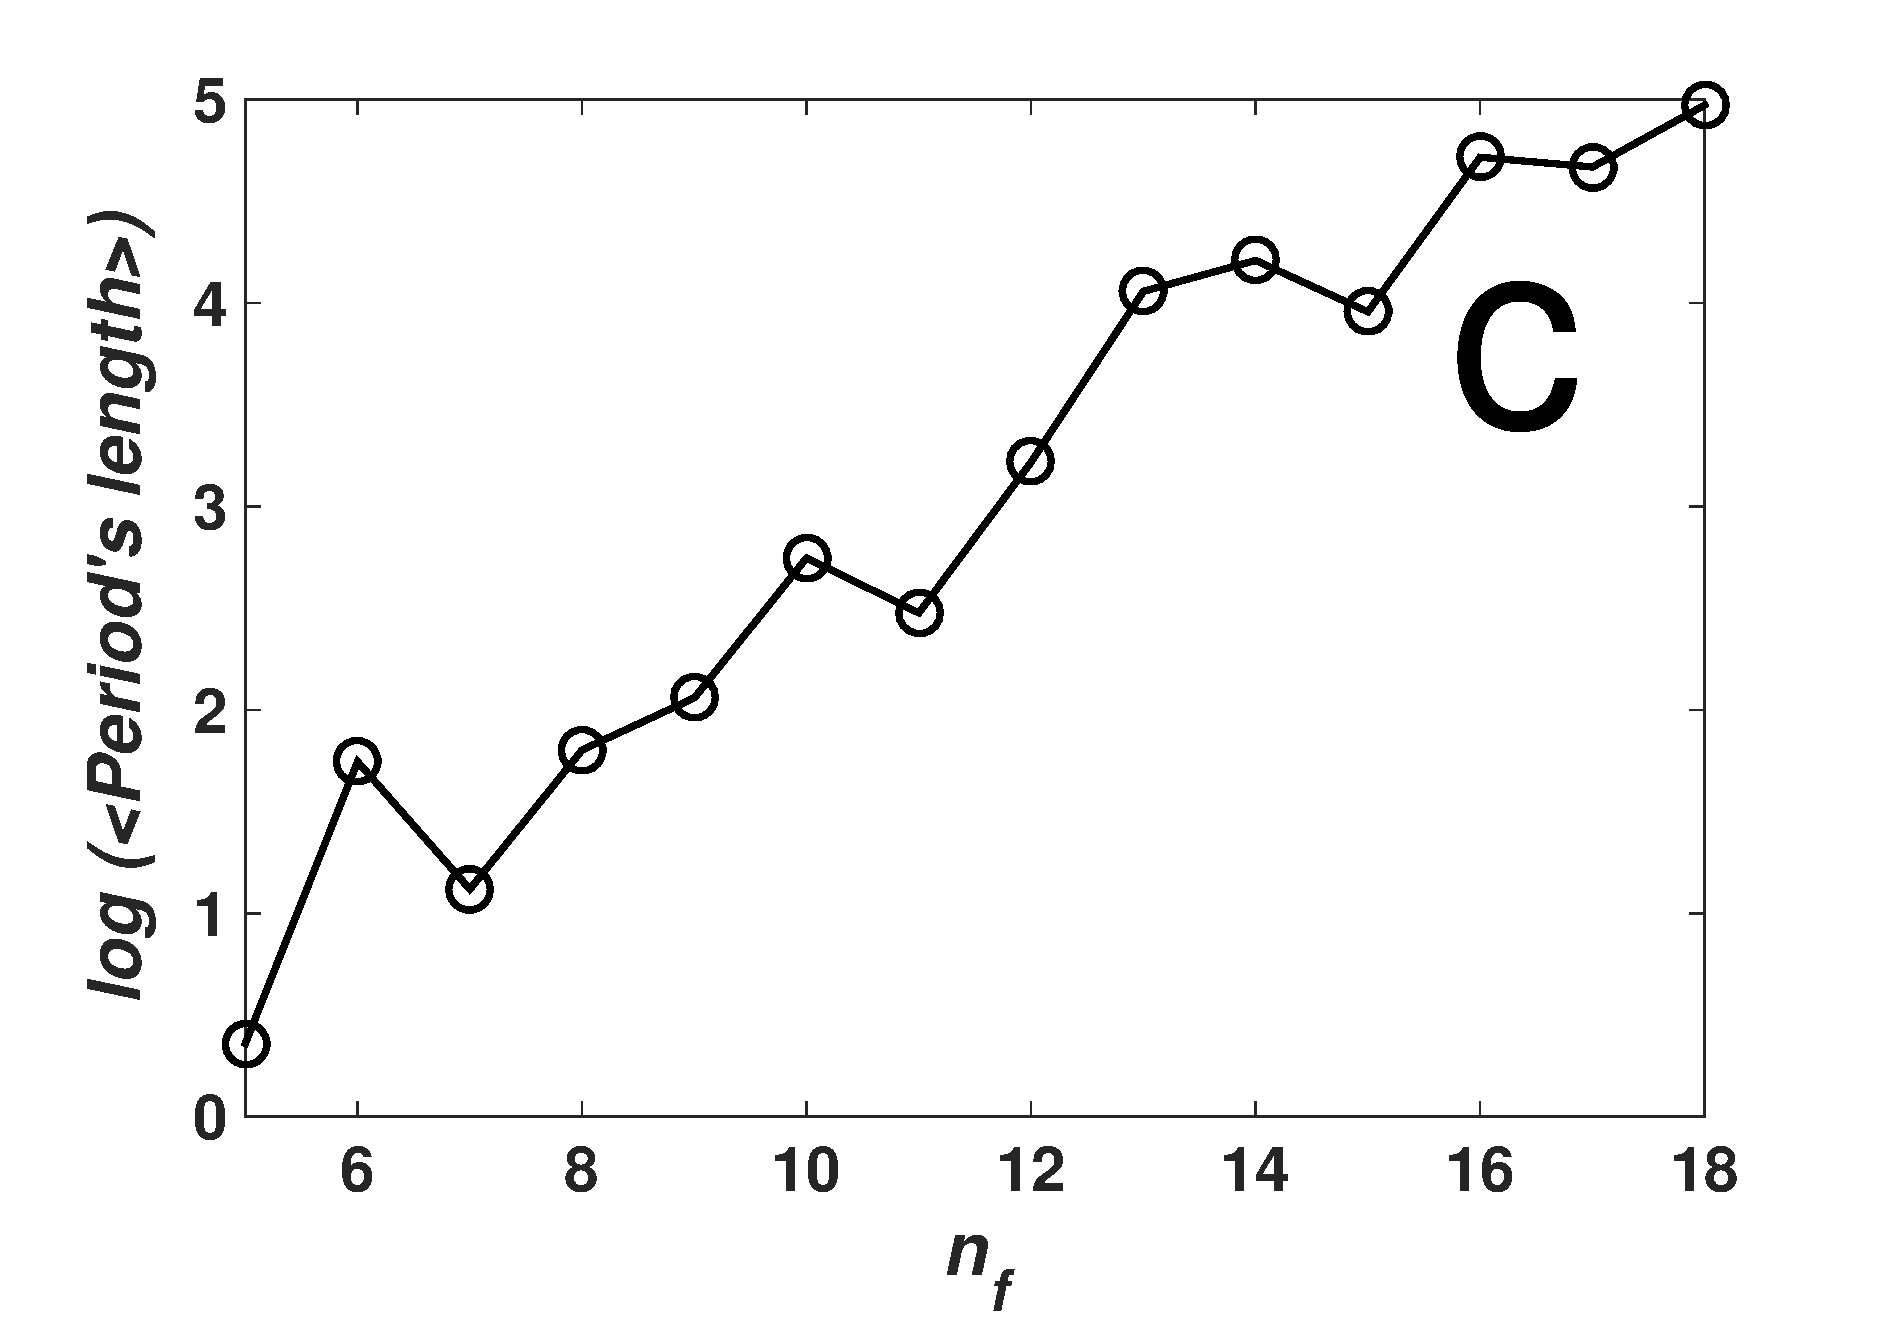
\includegraphics[width=0.48\textwidth]{Periodos_prom}
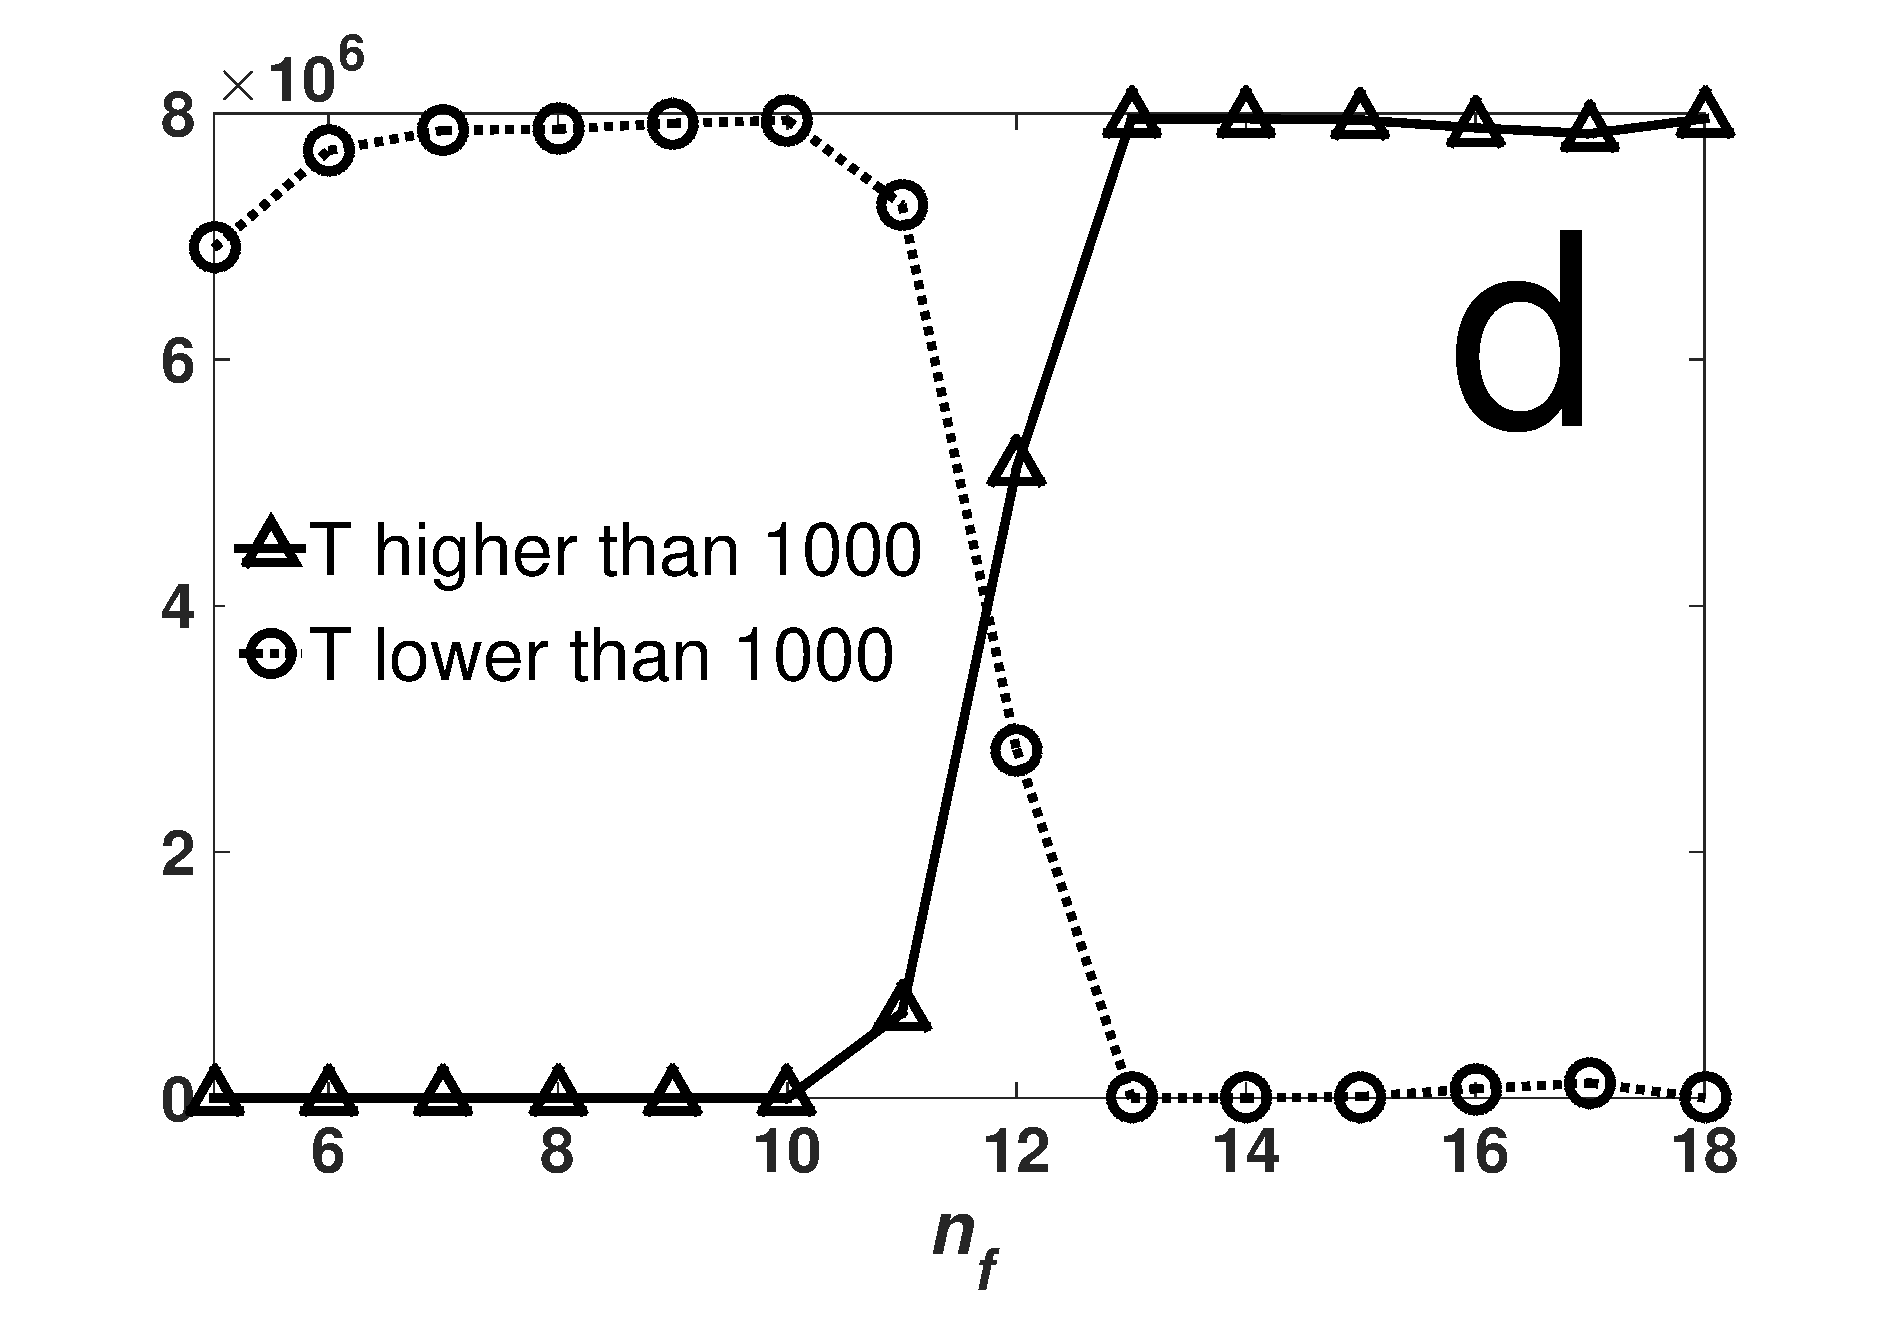
\includegraphics[width=0.48\textwidth]{Puntos}
\end{tabular}
\caption{Summary of initial conditions' behavior:
(a) number of fixed points; (b) number of divergent points; (c) logarithm of the length's cycles weighted average;  (d) initial conditions with period length higher and lower than $1,000$.}
\label{puntos}
\end{figure}
%============================================================================================
%==================================================
\begin{figure}
    \centering
        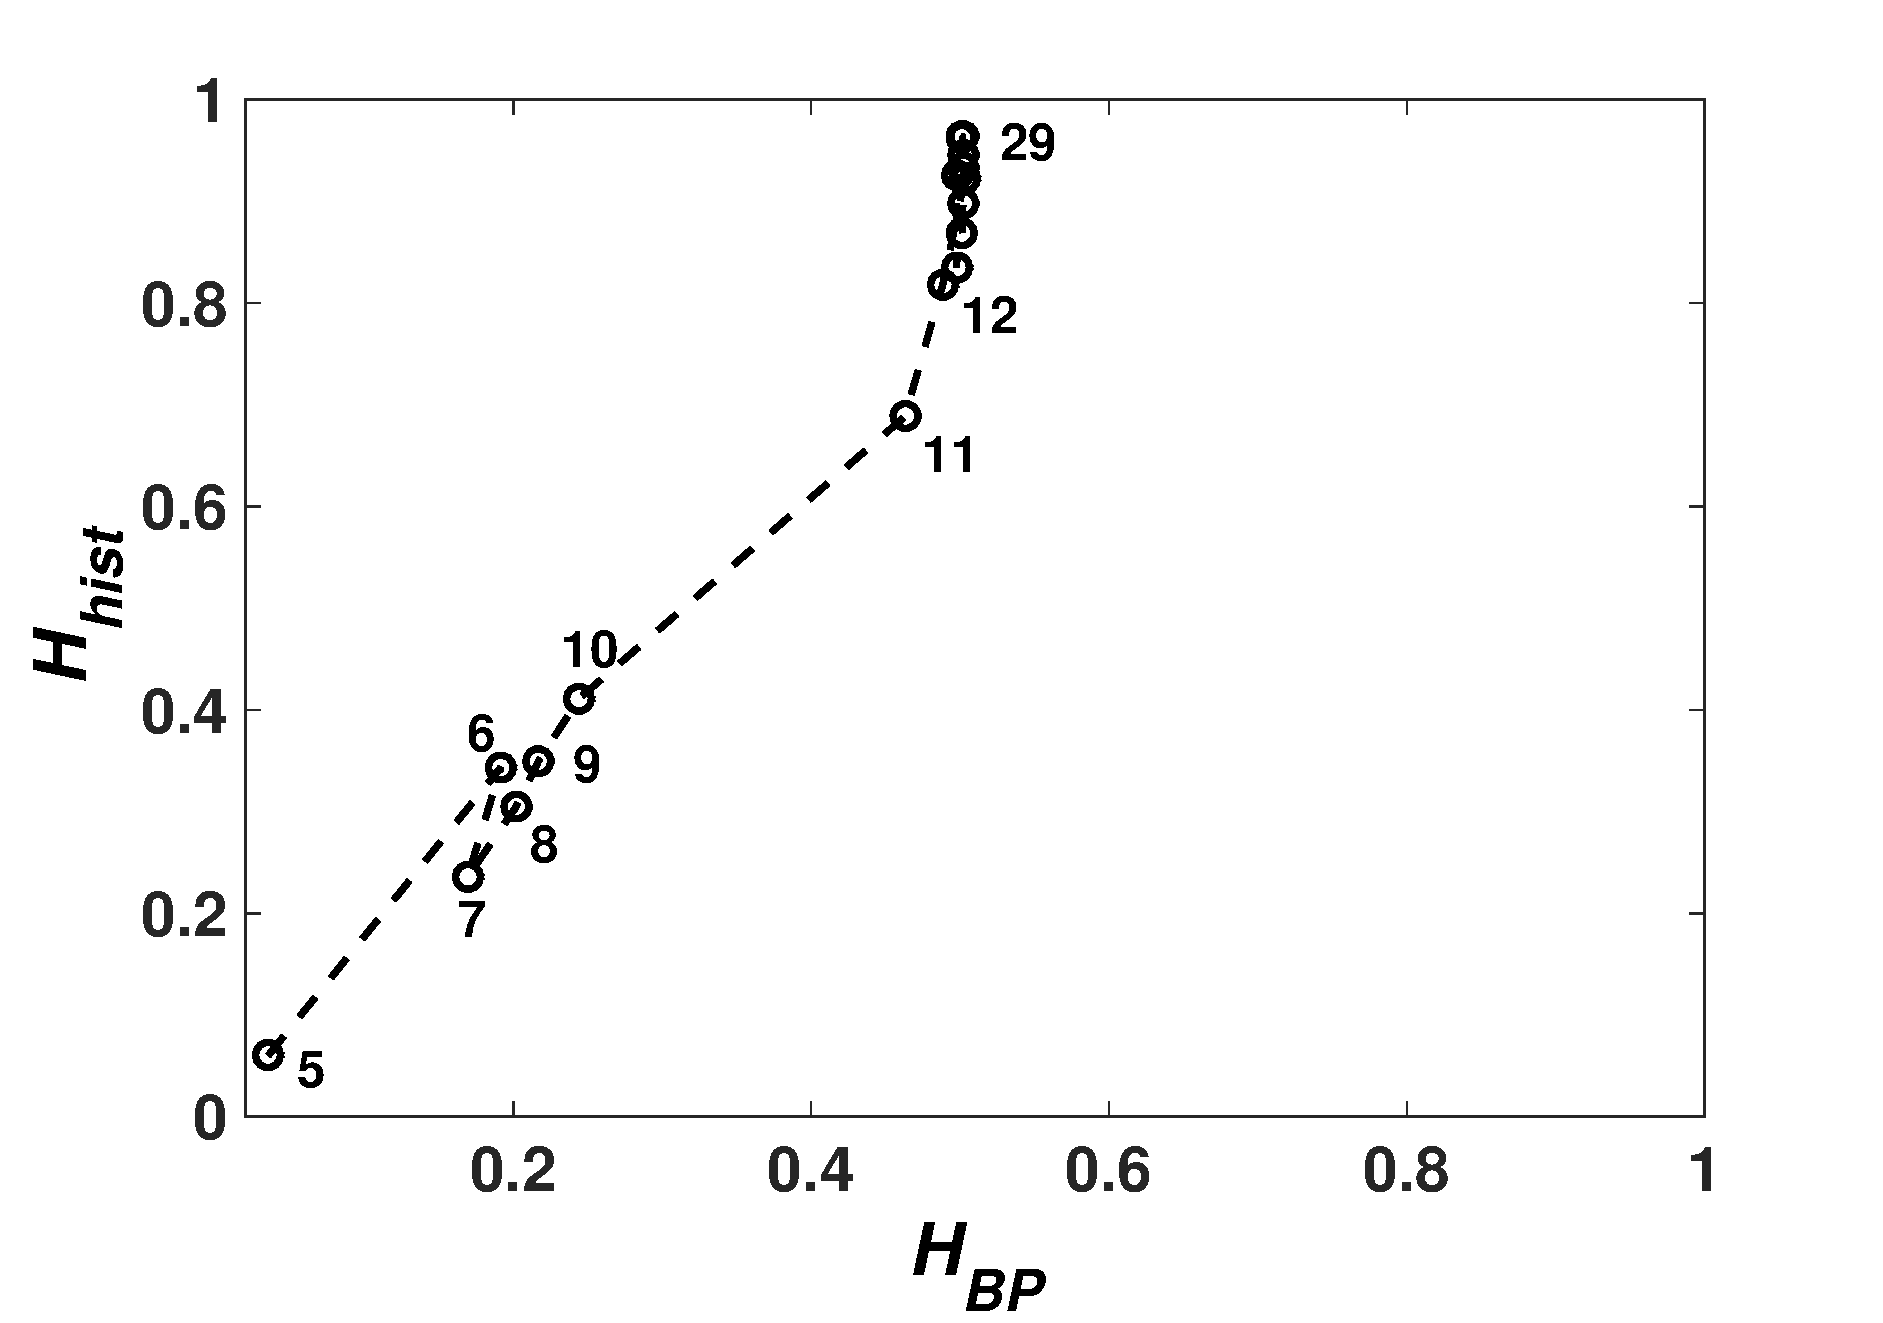
\includegraphics[width=0.7\columnwidth]{HBPvsHhist}\\
    \caption{Plane $H_{hist}$ - $H_{BP}$  for different number of bits. }\label{fig:HBPvsHhist}
\end{figure}


\begin{figure}
    \centering
        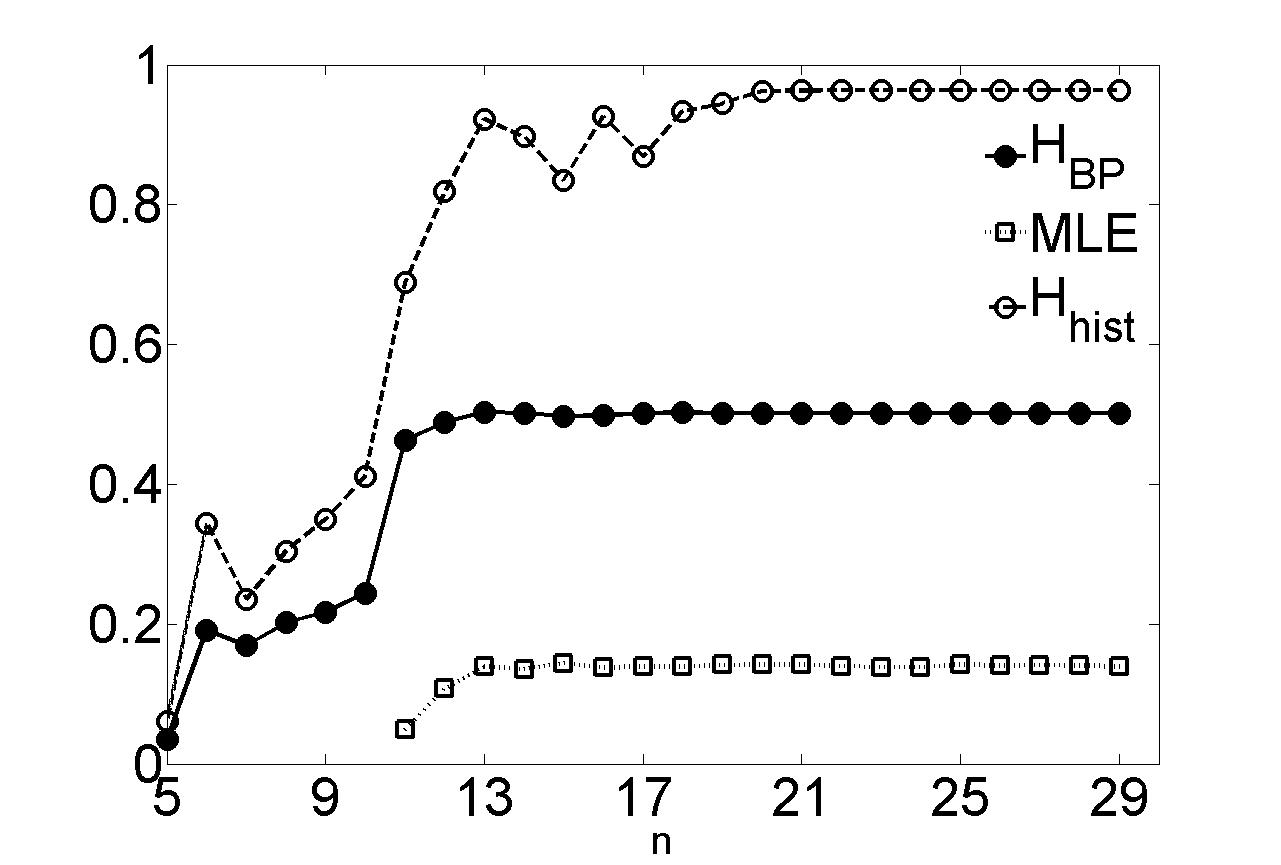
\includegraphics[width=0.7\columnwidth]{HBPHhist}\\
    \caption{Weighted average of quantifiers $H_{BP}$,  $H_{hist}$ and \textsl{MLE} as functions of the number of bits.}\label{fig:HBPHhist}
\end{figure}

Finally, Fig. \ref{puntos}.d shows the number of initial conditions that
presents periods $T$ higher and lower than $1,000$. Again, a value
of $12$ for $n_f$ seems to be the limit to obtain a good
approximation of the system.

Table \ref{tabla:MLE} shows the calculated \textsl{MLE} for some values of $n_f$. It can be seen that, as expected, while $n_f$ increases the \textsl{MLE} tends to its theoretical value.
 
\begin{table}[!t]\label{tabla:MLE}
\begin{center}
\caption{\textsl{MLE} for different values of $n_f$.}
\label{tabla:MLE}
\begin{tabular}{l l}

  \hline

  $n_f$ & \textsl{MLE} \\
  \hline
  \hline
  $11$ & $0.049214459144086$ \\
  $12$ & $0.107498218078192$ \\
  $13$ & $0.139472468153184$ \\
  $14$ & $ 0.135756935006498$ \\
  $15$ & $0.144155039896011$ \\
  $16$ & $0.137514471652835$ \\
  $25$ & $0.142134613438658$ \\
  $27$ & $0.141180317168284$ \\
  float & $0.142275657734227$ \\
   \hline

\end{tabular}
\end{center}

\end{table}